\subsection{Galvanic skin reaction and temperature data;}
\label{subsec:results_gsr_temp}

The GSR analysis is made by analyzing the average in each round and comparing it with the "Baseline" average. The temperature was analyzed with the GSR to see if there is some influence and by a graphical analysis there was none.

\subsubsection{Analysis of the GSR average}

The Table \ref{tab:gsr_avg_table} presents the average skin conductance by each participant on each scenes and they are plotted in the Figures \ref{fig:barplot_gsr_scene_blind} and \ref{fig:barplot_gsr_scene_sight}. It is possible to see that in all of the methods there was an increase in the average skin conductance, meaning that the user was aroused and maybe an increase in the mental workload.


\begin{table}[!htb]
\centering
\caption{Average GSR felled by the participants.}
\label{tab:gsr_avg_table}
\begin{tabular}{lllrrrrrr}
\toprule
    &       &        & Baseline &   Base &  Audio & \begin{tabular}[c]{@{}l@{}}Haptic\\ Belt\end{tabular} & \begin{tabular}[c]{@{}l@{}}Virtual\\ Cane\end{tabular} & Mixture \\
Participant & Visual Condition & Round &          &        &        &                                                       &                                                        &         \\
\midrule
001 & Sight & First &     4.27 &   8.80 &  15.19 &                                                 15.67 &                                                  15.19 &   14.15 \\
    &       & Return &          &  11.48 &  14.95 &                                                 15.09 &                                                  15.72 &   21.52 \\
001C & Blind & First &     0.37 &   0.48 &   1.03 &                                                  3.14 &                                                   3.79 &    3.90 \\
    &       & Return &          &   0.83 &   1.58 &                                                  2.81 &                                                   4.04 &    4.57 \\
002C & Blind & First &     0.17 &   0.91 &   0.23 &                                                  0.17 &                                                   0.17 &    0.17 \\
    &       & Return &          &   0.43 &   0.17 &                                                  0.16 &                                                   0.17 &    0.17 \\
003 & Sight & First &     0.19 &   0.19 &   0.17 &                                                  0.17 &                                                   0.17 &    0.17 \\
    &       & Return &          &   0.17 &   0.17 &                                                  0.17 &                                                   0.17 &    0.17 \\
003C & Blind & First &     0.30 &   0.56 &   0.56 &                                                  0.62 &                                                   0.85 &    1.09 \\
    &       & Return &          &   0.62 &   0.63 &                                                  0.65 &                                                   0.92 &    1.06 \\
004 & Sight & First &     2.60 &   9.71 &  11.18 &                                                 12.60 &                                                  12.92 &   10.34 \\
    &       & Return &          &  10.89 &  11.97 &                                                 12.25 &                                                  13.47 &   10.16 \\
004C & Blind & First &     1.24 &   2.34 &   3.07 &                                                  3.49 &                                                   2.28 &    2.23 \\
    &       & Return &          &   2.57 &   2.95 &                                                  3.20 &                                                   2.21 &    2.24 \\
005 & Sight & First &     0.47 &   1.88 &   1.58 &                                                  1.44 &                                                   1.37 &    1.33 \\
    &       & Return &          &   1.66 &   1.53 &                                                  1.47 &                                                   1.49 &    1.33 \\
\bottomrule
\end{tabular}
\end{table}



\begin{figure}[!htb]
    \centering
    \begin{minipage}{\textwidth}
        \centering
        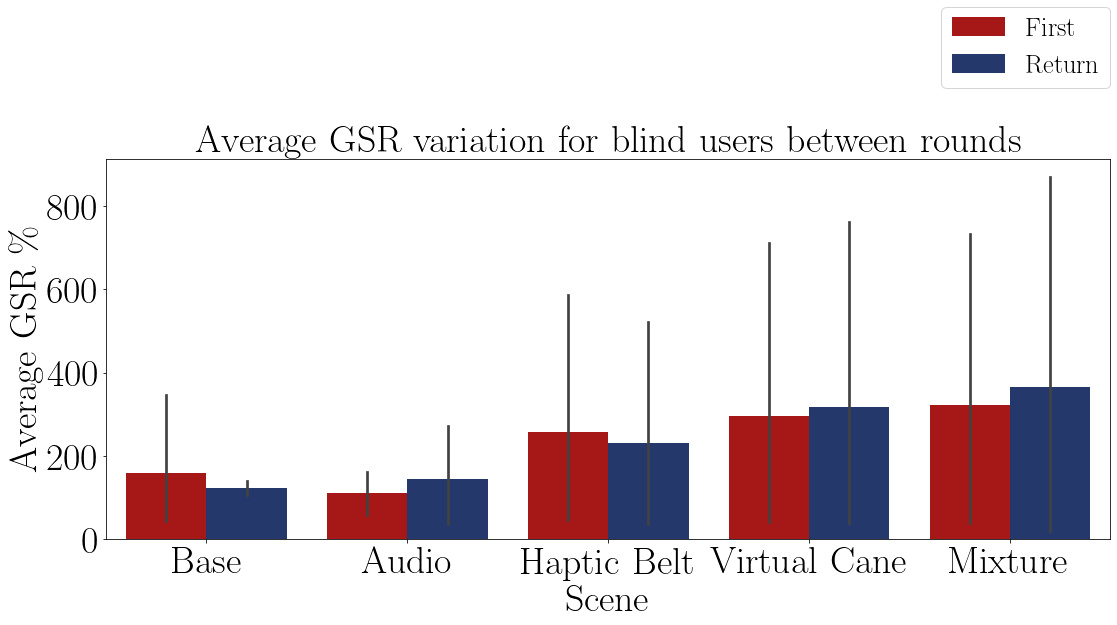
\includegraphics[width = 0.8\linewidth]{Resultados/GSR/Figuras/png/barplot_gsr_avg_scene_blind.png}
        %\resizebox{0.8\linewidth}{!}{
        %%% Creator: Matplotlib, PGF backend
%%
%% To include the figure in your LaTeX document, write
%%   \input{<filename>.pgf}
%%
%% Make sure the required packages are loaded in your preamble
%%   \usepackage{pgf}
%%
%% Figures using additional raster images can only be included by \input if
%% they are in the same directory as the main LaTeX file. For loading figures
%% from other directories you can use the `import` package
%%   \usepackage{import}
%%
%% and then include the figures with
%%   \import{<path to file>}{<filename>.pgf}
%%
%% Matplotlib used the following preamble
%%   \usepackage{fontspec}
%%
\begingroup%
\makeatletter%
\begin{pgfpicture}%
\pgfpathrectangle{\pgfpointorigin}{\pgfqpoint{15.369508in}{8.690562in}}%
\pgfusepath{use as bounding box, clip}%
\begin{pgfscope}%
\pgfsetbuttcap%
\pgfsetmiterjoin%
\pgfsetlinewidth{0.000000pt}%
\definecolor{currentstroke}{rgb}{1.000000,1.000000,1.000000}%
\pgfsetstrokecolor{currentstroke}%
\pgfsetstrokeopacity{0.000000}%
\pgfsetdash{}{0pt}%
\pgfpathmoveto{\pgfqpoint{0.000000in}{-0.000000in}}%
\pgfpathlineto{\pgfqpoint{15.369508in}{-0.000000in}}%
\pgfpathlineto{\pgfqpoint{15.369508in}{8.690562in}}%
\pgfpathlineto{\pgfqpoint{0.000000in}{8.690562in}}%
\pgfpathclose%
\pgfusepath{}%
\end{pgfscope}%
\begin{pgfscope}%
\pgfsetbuttcap%
\pgfsetmiterjoin%
\definecolor{currentfill}{rgb}{1.000000,1.000000,1.000000}%
\pgfsetfillcolor{currentfill}%
\pgfsetlinewidth{0.000000pt}%
\definecolor{currentstroke}{rgb}{0.000000,0.000000,0.000000}%
\pgfsetstrokecolor{currentstroke}%
\pgfsetstrokeopacity{0.000000}%
\pgfsetdash{}{0pt}%
\pgfpathmoveto{\pgfqpoint{1.319508in}{1.191562in}}%
\pgfpathlineto{\pgfqpoint{15.269508in}{1.191562in}}%
\pgfpathlineto{\pgfqpoint{15.269508in}{6.476562in}}%
\pgfpathlineto{\pgfqpoint{1.319508in}{6.476562in}}%
\pgfpathclose%
\pgfusepath{fill}%
\end{pgfscope}%
\begin{pgfscope}%
\pgfpathrectangle{\pgfqpoint{1.319508in}{1.191562in}}{\pgfqpoint{13.950000in}{5.285000in}}%
\pgfusepath{clip}%
\pgfsetbuttcap%
\pgfsetmiterjoin%
\definecolor{currentfill}{rgb}{0.651961,0.093137,0.093137}%
\pgfsetfillcolor{currentfill}%
\pgfsetlinewidth{0.000000pt}%
\definecolor{currentstroke}{rgb}{0.000000,0.000000,0.000000}%
\pgfsetstrokecolor{currentstroke}%
\pgfsetstrokeopacity{0.000000}%
\pgfsetdash{}{0pt}%
\pgfpathmoveto{\pgfqpoint{1.598508in}{5.432025in}}%
\pgfpathlineto{\pgfqpoint{2.714508in}{5.432025in}}%
\pgfpathlineto{\pgfqpoint{2.714508in}{4.583309in}}%
\pgfpathlineto{\pgfqpoint{1.598508in}{4.583309in}}%
\pgfpathclose%
\pgfusepath{fill}%
\end{pgfscope}%
\begin{pgfscope}%
\pgfpathrectangle{\pgfqpoint{1.319508in}{1.191562in}}{\pgfqpoint{13.950000in}{5.285000in}}%
\pgfusepath{clip}%
\pgfsetbuttcap%
\pgfsetmiterjoin%
\definecolor{currentfill}{rgb}{0.651961,0.093137,0.093137}%
\pgfsetfillcolor{currentfill}%
\pgfsetlinewidth{0.000000pt}%
\definecolor{currentstroke}{rgb}{0.000000,0.000000,0.000000}%
\pgfsetstrokecolor{currentstroke}%
\pgfsetstrokeopacity{0.000000}%
\pgfsetdash{}{0pt}%
\pgfpathmoveto{\pgfqpoint{4.388508in}{5.432025in}}%
\pgfpathlineto{\pgfqpoint{5.504508in}{5.432025in}}%
\pgfpathlineto{\pgfqpoint{5.504508in}{3.558465in}}%
\pgfpathlineto{\pgfqpoint{4.388508in}{3.558465in}}%
\pgfpathclose%
\pgfusepath{fill}%
\end{pgfscope}%
\begin{pgfscope}%
\pgfpathrectangle{\pgfqpoint{1.319508in}{1.191562in}}{\pgfqpoint{13.950000in}{5.285000in}}%
\pgfusepath{clip}%
\pgfsetbuttcap%
\pgfsetmiterjoin%
\definecolor{currentfill}{rgb}{0.651961,0.093137,0.093137}%
\pgfsetfillcolor{currentfill}%
\pgfsetlinewidth{0.000000pt}%
\definecolor{currentstroke}{rgb}{0.000000,0.000000,0.000000}%
\pgfsetstrokecolor{currentstroke}%
\pgfsetstrokeopacity{0.000000}%
\pgfsetdash{}{0pt}%
\pgfpathmoveto{\pgfqpoint{7.178508in}{5.432025in}}%
\pgfpathlineto{\pgfqpoint{8.294508in}{5.432025in}}%
\pgfpathlineto{\pgfqpoint{8.294508in}{4.476572in}}%
\pgfpathlineto{\pgfqpoint{7.178508in}{4.476572in}}%
\pgfpathclose%
\pgfusepath{fill}%
\end{pgfscope}%
\begin{pgfscope}%
\pgfpathrectangle{\pgfqpoint{1.319508in}{1.191562in}}{\pgfqpoint{13.950000in}{5.285000in}}%
\pgfusepath{clip}%
\pgfsetbuttcap%
\pgfsetmiterjoin%
\definecolor{currentfill}{rgb}{0.651961,0.093137,0.093137}%
\pgfsetfillcolor{currentfill}%
\pgfsetlinewidth{0.000000pt}%
\definecolor{currentstroke}{rgb}{0.000000,0.000000,0.000000}%
\pgfsetstrokecolor{currentstroke}%
\pgfsetstrokeopacity{0.000000}%
\pgfsetdash{}{0pt}%
\pgfpathmoveto{\pgfqpoint{9.968508in}{5.432025in}}%
\pgfpathlineto{\pgfqpoint{11.084508in}{5.432025in}}%
\pgfpathlineto{\pgfqpoint{11.084508in}{3.778608in}}%
\pgfpathlineto{\pgfqpoint{9.968508in}{3.778608in}}%
\pgfpathclose%
\pgfusepath{fill}%
\end{pgfscope}%
\begin{pgfscope}%
\pgfpathrectangle{\pgfqpoint{1.319508in}{1.191562in}}{\pgfqpoint{13.950000in}{5.285000in}}%
\pgfusepath{clip}%
\pgfsetbuttcap%
\pgfsetmiterjoin%
\definecolor{currentfill}{rgb}{0.651961,0.093137,0.093137}%
\pgfsetfillcolor{currentfill}%
\pgfsetlinewidth{0.000000pt}%
\definecolor{currentstroke}{rgb}{0.000000,0.000000,0.000000}%
\pgfsetstrokecolor{currentstroke}%
\pgfsetstrokeopacity{0.000000}%
\pgfsetdash{}{0pt}%
\pgfpathmoveto{\pgfqpoint{12.758508in}{5.432025in}}%
\pgfpathlineto{\pgfqpoint{13.874508in}{5.432025in}}%
\pgfpathlineto{\pgfqpoint{13.874508in}{4.339698in}}%
\pgfpathlineto{\pgfqpoint{12.758508in}{4.339698in}}%
\pgfpathclose%
\pgfusepath{fill}%
\end{pgfscope}%
\begin{pgfscope}%
\pgfpathrectangle{\pgfqpoint{1.319508in}{1.191562in}}{\pgfqpoint{13.950000in}{5.285000in}}%
\pgfusepath{clip}%
\pgfsetbuttcap%
\pgfsetmiterjoin%
\definecolor{currentfill}{rgb}{0.144608,0.218137,0.424020}%
\pgfsetfillcolor{currentfill}%
\pgfsetlinewidth{0.000000pt}%
\definecolor{currentstroke}{rgb}{0.000000,0.000000,0.000000}%
\pgfsetstrokecolor{currentstroke}%
\pgfsetstrokeopacity{0.000000}%
\pgfsetdash{}{0pt}%
\pgfpathmoveto{\pgfqpoint{2.714508in}{5.432025in}}%
\pgfpathlineto{\pgfqpoint{3.830508in}{5.432025in}}%
\pgfpathlineto{\pgfqpoint{3.830508in}{4.506389in}}%
\pgfpathlineto{\pgfqpoint{2.714508in}{4.506389in}}%
\pgfpathclose%
\pgfusepath{fill}%
\end{pgfscope}%
\begin{pgfscope}%
\pgfpathrectangle{\pgfqpoint{1.319508in}{1.191562in}}{\pgfqpoint{13.950000in}{5.285000in}}%
\pgfusepath{clip}%
\pgfsetbuttcap%
\pgfsetmiterjoin%
\definecolor{currentfill}{rgb}{0.144608,0.218137,0.424020}%
\pgfsetfillcolor{currentfill}%
\pgfsetlinewidth{0.000000pt}%
\definecolor{currentstroke}{rgb}{0.000000,0.000000,0.000000}%
\pgfsetstrokecolor{currentstroke}%
\pgfsetstrokeopacity{0.000000}%
\pgfsetdash{}{0pt}%
\pgfpathmoveto{\pgfqpoint{5.504508in}{5.432025in}}%
\pgfpathlineto{\pgfqpoint{6.620508in}{5.432025in}}%
\pgfpathlineto{\pgfqpoint{6.620508in}{3.808164in}}%
\pgfpathlineto{\pgfqpoint{5.504508in}{3.808164in}}%
\pgfpathclose%
\pgfusepath{fill}%
\end{pgfscope}%
\begin{pgfscope}%
\pgfpathrectangle{\pgfqpoint{1.319508in}{1.191562in}}{\pgfqpoint{13.950000in}{5.285000in}}%
\pgfusepath{clip}%
\pgfsetbuttcap%
\pgfsetmiterjoin%
\definecolor{currentfill}{rgb}{0.144608,0.218137,0.424020}%
\pgfsetfillcolor{currentfill}%
\pgfsetlinewidth{0.000000pt}%
\definecolor{currentstroke}{rgb}{0.000000,0.000000,0.000000}%
\pgfsetstrokecolor{currentstroke}%
\pgfsetstrokeopacity{0.000000}%
\pgfsetdash{}{0pt}%
\pgfpathmoveto{\pgfqpoint{8.294508in}{5.432025in}}%
\pgfpathlineto{\pgfqpoint{9.410508in}{5.432025in}}%
\pgfpathlineto{\pgfqpoint{9.410508in}{4.696413in}}%
\pgfpathlineto{\pgfqpoint{8.294508in}{4.696413in}}%
\pgfpathclose%
\pgfusepath{fill}%
\end{pgfscope}%
\begin{pgfscope}%
\pgfpathrectangle{\pgfqpoint{1.319508in}{1.191562in}}{\pgfqpoint{13.950000in}{5.285000in}}%
\pgfusepath{clip}%
\pgfsetbuttcap%
\pgfsetmiterjoin%
\definecolor{currentfill}{rgb}{0.144608,0.218137,0.424020}%
\pgfsetfillcolor{currentfill}%
\pgfsetlinewidth{0.000000pt}%
\definecolor{currentstroke}{rgb}{0.000000,0.000000,0.000000}%
\pgfsetstrokecolor{currentstroke}%
\pgfsetstrokeopacity{0.000000}%
\pgfsetdash{}{0pt}%
\pgfpathmoveto{\pgfqpoint{11.084508in}{5.432025in}}%
\pgfpathlineto{\pgfqpoint{12.200508in}{5.432025in}}%
\pgfpathlineto{\pgfqpoint{12.200508in}{4.423975in}}%
\pgfpathlineto{\pgfqpoint{11.084508in}{4.423975in}}%
\pgfpathclose%
\pgfusepath{fill}%
\end{pgfscope}%
\begin{pgfscope}%
\pgfpathrectangle{\pgfqpoint{1.319508in}{1.191562in}}{\pgfqpoint{13.950000in}{5.285000in}}%
\pgfusepath{clip}%
\pgfsetbuttcap%
\pgfsetmiterjoin%
\definecolor{currentfill}{rgb}{0.144608,0.218137,0.424020}%
\pgfsetfillcolor{currentfill}%
\pgfsetlinewidth{0.000000pt}%
\definecolor{currentstroke}{rgb}{0.000000,0.000000,0.000000}%
\pgfsetstrokecolor{currentstroke}%
\pgfsetstrokeopacity{0.000000}%
\pgfsetdash{}{0pt}%
\pgfpathmoveto{\pgfqpoint{13.874508in}{5.432025in}}%
\pgfpathlineto{\pgfqpoint{14.990508in}{5.432025in}}%
\pgfpathlineto{\pgfqpoint{14.990508in}{4.469000in}}%
\pgfpathlineto{\pgfqpoint{13.874508in}{4.469000in}}%
\pgfpathclose%
\pgfusepath{fill}%
\end{pgfscope}%
\begin{pgfscope}%
\pgfsetbuttcap%
\pgfsetroundjoin%
\definecolor{currentfill}{rgb}{0.000000,0.000000,0.000000}%
\pgfsetfillcolor{currentfill}%
\pgfsetlinewidth{0.803000pt}%
\definecolor{currentstroke}{rgb}{0.000000,0.000000,0.000000}%
\pgfsetstrokecolor{currentstroke}%
\pgfsetdash{}{0pt}%
\pgfsys@defobject{currentmarker}{\pgfqpoint{0.000000in}{-0.048611in}}{\pgfqpoint{0.000000in}{0.000000in}}{%
\pgfpathmoveto{\pgfqpoint{0.000000in}{0.000000in}}%
\pgfpathlineto{\pgfqpoint{0.000000in}{-0.048611in}}%
\pgfusepath{stroke,fill}%
}%
\begin{pgfscope}%
\pgfsys@transformshift{2.714508in}{1.191562in}%
\pgfsys@useobject{currentmarker}{}%
\end{pgfscope}%
\end{pgfscope}%
\begin{pgfscope}%
\definecolor{textcolor}{rgb}{0.000000,0.000000,0.000000}%
\pgfsetstrokecolor{textcolor}%
\pgfsetfillcolor{textcolor}%
\pgftext[x=2.714508in,y=1.094339in,,top]{\color{textcolor}\rmfamily\fontsize{38.016000}{45.619200}\selectfont Base}%
\end{pgfscope}%
\begin{pgfscope}%
\pgfsetbuttcap%
\pgfsetroundjoin%
\definecolor{currentfill}{rgb}{0.000000,0.000000,0.000000}%
\pgfsetfillcolor{currentfill}%
\pgfsetlinewidth{0.803000pt}%
\definecolor{currentstroke}{rgb}{0.000000,0.000000,0.000000}%
\pgfsetstrokecolor{currentstroke}%
\pgfsetdash{}{0pt}%
\pgfsys@defobject{currentmarker}{\pgfqpoint{0.000000in}{-0.048611in}}{\pgfqpoint{0.000000in}{0.000000in}}{%
\pgfpathmoveto{\pgfqpoint{0.000000in}{0.000000in}}%
\pgfpathlineto{\pgfqpoint{0.000000in}{-0.048611in}}%
\pgfusepath{stroke,fill}%
}%
\begin{pgfscope}%
\pgfsys@transformshift{5.504508in}{1.191562in}%
\pgfsys@useobject{currentmarker}{}%
\end{pgfscope}%
\end{pgfscope}%
\begin{pgfscope}%
\definecolor{textcolor}{rgb}{0.000000,0.000000,0.000000}%
\pgfsetstrokecolor{textcolor}%
\pgfsetfillcolor{textcolor}%
\pgftext[x=5.504508in,y=1.094339in,,top]{\color{textcolor}\rmfamily\fontsize{38.016000}{45.619200}\selectfont Audio}%
\end{pgfscope}%
\begin{pgfscope}%
\pgfsetbuttcap%
\pgfsetroundjoin%
\definecolor{currentfill}{rgb}{0.000000,0.000000,0.000000}%
\pgfsetfillcolor{currentfill}%
\pgfsetlinewidth{0.803000pt}%
\definecolor{currentstroke}{rgb}{0.000000,0.000000,0.000000}%
\pgfsetstrokecolor{currentstroke}%
\pgfsetdash{}{0pt}%
\pgfsys@defobject{currentmarker}{\pgfqpoint{0.000000in}{-0.048611in}}{\pgfqpoint{0.000000in}{0.000000in}}{%
\pgfpathmoveto{\pgfqpoint{0.000000in}{0.000000in}}%
\pgfpathlineto{\pgfqpoint{0.000000in}{-0.048611in}}%
\pgfusepath{stroke,fill}%
}%
\begin{pgfscope}%
\pgfsys@transformshift{8.294508in}{1.191562in}%
\pgfsys@useobject{currentmarker}{}%
\end{pgfscope}%
\end{pgfscope}%
\begin{pgfscope}%
\definecolor{textcolor}{rgb}{0.000000,0.000000,0.000000}%
\pgfsetstrokecolor{textcolor}%
\pgfsetfillcolor{textcolor}%
\pgftext[x=8.294508in,y=1.094339in,,top]{\color{textcolor}\rmfamily\fontsize{38.016000}{45.619200}\selectfont Haptic Belt}%
\end{pgfscope}%
\begin{pgfscope}%
\pgfsetbuttcap%
\pgfsetroundjoin%
\definecolor{currentfill}{rgb}{0.000000,0.000000,0.000000}%
\pgfsetfillcolor{currentfill}%
\pgfsetlinewidth{0.803000pt}%
\definecolor{currentstroke}{rgb}{0.000000,0.000000,0.000000}%
\pgfsetstrokecolor{currentstroke}%
\pgfsetdash{}{0pt}%
\pgfsys@defobject{currentmarker}{\pgfqpoint{0.000000in}{-0.048611in}}{\pgfqpoint{0.000000in}{0.000000in}}{%
\pgfpathmoveto{\pgfqpoint{0.000000in}{0.000000in}}%
\pgfpathlineto{\pgfqpoint{0.000000in}{-0.048611in}}%
\pgfusepath{stroke,fill}%
}%
\begin{pgfscope}%
\pgfsys@transformshift{11.084508in}{1.191562in}%
\pgfsys@useobject{currentmarker}{}%
\end{pgfscope}%
\end{pgfscope}%
\begin{pgfscope}%
\definecolor{textcolor}{rgb}{0.000000,0.000000,0.000000}%
\pgfsetstrokecolor{textcolor}%
\pgfsetfillcolor{textcolor}%
\pgftext[x=11.084508in,y=1.094339in,,top]{\color{textcolor}\rmfamily\fontsize{38.016000}{45.619200}\selectfont Virtual Cane}%
\end{pgfscope}%
\begin{pgfscope}%
\pgfsetbuttcap%
\pgfsetroundjoin%
\definecolor{currentfill}{rgb}{0.000000,0.000000,0.000000}%
\pgfsetfillcolor{currentfill}%
\pgfsetlinewidth{0.803000pt}%
\definecolor{currentstroke}{rgb}{0.000000,0.000000,0.000000}%
\pgfsetstrokecolor{currentstroke}%
\pgfsetdash{}{0pt}%
\pgfsys@defobject{currentmarker}{\pgfqpoint{0.000000in}{-0.048611in}}{\pgfqpoint{0.000000in}{0.000000in}}{%
\pgfpathmoveto{\pgfqpoint{0.000000in}{0.000000in}}%
\pgfpathlineto{\pgfqpoint{0.000000in}{-0.048611in}}%
\pgfusepath{stroke,fill}%
}%
\begin{pgfscope}%
\pgfsys@transformshift{13.874508in}{1.191562in}%
\pgfsys@useobject{currentmarker}{}%
\end{pgfscope}%
\end{pgfscope}%
\begin{pgfscope}%
\definecolor{textcolor}{rgb}{0.000000,0.000000,0.000000}%
\pgfsetstrokecolor{textcolor}%
\pgfsetfillcolor{textcolor}%
\pgftext[x=13.874508in,y=1.094339in,,top]{\color{textcolor}\rmfamily\fontsize{38.016000}{45.619200}\selectfont Mixture}%
\end{pgfscope}%
\begin{pgfscope}%
\definecolor{textcolor}{rgb}{0.000000,0.000000,0.000000}%
\pgfsetstrokecolor{textcolor}%
\pgfsetfillcolor{textcolor}%
\pgftext[x=8.294508in,y=0.569392in,,top]{\color{textcolor}\rmfamily\fontsize{38.016000}{45.619200}\selectfont Scene}%
\end{pgfscope}%
\begin{pgfscope}%
\pgfsetbuttcap%
\pgfsetroundjoin%
\definecolor{currentfill}{rgb}{0.000000,0.000000,0.000000}%
\pgfsetfillcolor{currentfill}%
\pgfsetlinewidth{0.803000pt}%
\definecolor{currentstroke}{rgb}{0.000000,0.000000,0.000000}%
\pgfsetstrokecolor{currentstroke}%
\pgfsetdash{}{0pt}%
\pgfsys@defobject{currentmarker}{\pgfqpoint{-0.048611in}{0.000000in}}{\pgfqpoint{-0.000000in}{0.000000in}}{%
\pgfpathmoveto{\pgfqpoint{-0.000000in}{0.000000in}}%
\pgfpathlineto{\pgfqpoint{-0.048611in}{0.000000in}}%
\pgfusepath{stroke,fill}%
}%
\begin{pgfscope}%
\pgfsys@transformshift{1.319508in}{1.767373in}%
\pgfsys@useobject{currentmarker}{}%
\end{pgfscope}%
\end{pgfscope}%
\begin{pgfscope}%
\definecolor{textcolor}{rgb}{0.000000,0.000000,0.000000}%
\pgfsetstrokecolor{textcolor}%
\pgfsetfillcolor{textcolor}%
\pgftext[x=0.636563in, y=1.584157in, left, base]{\color{textcolor}\rmfamily\fontsize{38.016000}{45.619200}\selectfont \(\displaystyle {\ensuremath{-}30}\)}%
\end{pgfscope}%
\begin{pgfscope}%
\pgfsetbuttcap%
\pgfsetroundjoin%
\definecolor{currentfill}{rgb}{0.000000,0.000000,0.000000}%
\pgfsetfillcolor{currentfill}%
\pgfsetlinewidth{0.803000pt}%
\definecolor{currentstroke}{rgb}{0.000000,0.000000,0.000000}%
\pgfsetstrokecolor{currentstroke}%
\pgfsetdash{}{0pt}%
\pgfsys@defobject{currentmarker}{\pgfqpoint{-0.048611in}{0.000000in}}{\pgfqpoint{-0.000000in}{0.000000in}}{%
\pgfpathmoveto{\pgfqpoint{-0.000000in}{0.000000in}}%
\pgfpathlineto{\pgfqpoint{-0.048611in}{0.000000in}}%
\pgfusepath{stroke,fill}%
}%
\begin{pgfscope}%
\pgfsys@transformshift{1.319508in}{2.988924in}%
\pgfsys@useobject{currentmarker}{}%
\end{pgfscope}%
\end{pgfscope}%
\begin{pgfscope}%
\definecolor{textcolor}{rgb}{0.000000,0.000000,0.000000}%
\pgfsetstrokecolor{textcolor}%
\pgfsetfillcolor{textcolor}%
\pgftext[x=0.636563in, y=2.805708in, left, base]{\color{textcolor}\rmfamily\fontsize{38.016000}{45.619200}\selectfont \(\displaystyle {\ensuremath{-}20}\)}%
\end{pgfscope}%
\begin{pgfscope}%
\pgfsetbuttcap%
\pgfsetroundjoin%
\definecolor{currentfill}{rgb}{0.000000,0.000000,0.000000}%
\pgfsetfillcolor{currentfill}%
\pgfsetlinewidth{0.803000pt}%
\definecolor{currentstroke}{rgb}{0.000000,0.000000,0.000000}%
\pgfsetstrokecolor{currentstroke}%
\pgfsetdash{}{0pt}%
\pgfsys@defobject{currentmarker}{\pgfqpoint{-0.048611in}{0.000000in}}{\pgfqpoint{-0.000000in}{0.000000in}}{%
\pgfpathmoveto{\pgfqpoint{-0.000000in}{0.000000in}}%
\pgfpathlineto{\pgfqpoint{-0.048611in}{0.000000in}}%
\pgfusepath{stroke,fill}%
}%
\begin{pgfscope}%
\pgfsys@transformshift{1.319508in}{4.210475in}%
\pgfsys@useobject{currentmarker}{}%
\end{pgfscope}%
\end{pgfscope}%
\begin{pgfscope}%
\definecolor{textcolor}{rgb}{0.000000,0.000000,0.000000}%
\pgfsetstrokecolor{textcolor}%
\pgfsetfillcolor{textcolor}%
\pgftext[x=0.636563in, y=4.027258in, left, base]{\color{textcolor}\rmfamily\fontsize{38.016000}{45.619200}\selectfont \(\displaystyle {\ensuremath{-}10}\)}%
\end{pgfscope}%
\begin{pgfscope}%
\pgfsetbuttcap%
\pgfsetroundjoin%
\definecolor{currentfill}{rgb}{0.000000,0.000000,0.000000}%
\pgfsetfillcolor{currentfill}%
\pgfsetlinewidth{0.803000pt}%
\definecolor{currentstroke}{rgb}{0.000000,0.000000,0.000000}%
\pgfsetstrokecolor{currentstroke}%
\pgfsetdash{}{0pt}%
\pgfsys@defobject{currentmarker}{\pgfqpoint{-0.048611in}{0.000000in}}{\pgfqpoint{-0.000000in}{0.000000in}}{%
\pgfpathmoveto{\pgfqpoint{-0.000000in}{0.000000in}}%
\pgfpathlineto{\pgfqpoint{-0.048611in}{0.000000in}}%
\pgfusepath{stroke,fill}%
}%
\begin{pgfscope}%
\pgfsys@transformshift{1.319508in}{5.432025in}%
\pgfsys@useobject{currentmarker}{}%
\end{pgfscope}%
\end{pgfscope}%
\begin{pgfscope}%
\definecolor{textcolor}{rgb}{0.000000,0.000000,0.000000}%
\pgfsetstrokecolor{textcolor}%
\pgfsetfillcolor{textcolor}%
\pgftext[x=1.063808in, y=5.248809in, left, base]{\color{textcolor}\rmfamily\fontsize{38.016000}{45.619200}\selectfont \(\displaystyle {0}\)}%
\end{pgfscope}%
\begin{pgfscope}%
\definecolor{textcolor}{rgb}{0.000000,0.000000,0.000000}%
\pgfsetstrokecolor{textcolor}%
\pgfsetfillcolor{textcolor}%
\pgftext[x=0.581008in,y=3.834062in,,bottom,rotate=90.000000]{\color{textcolor}\rmfamily\fontsize{38.016000}{45.619200}\selectfont Average BPM}%
\end{pgfscope}%
\begin{pgfscope}%
\pgfpathrectangle{\pgfqpoint{1.319508in}{1.191562in}}{\pgfqpoint{13.950000in}{5.285000in}}%
\pgfusepath{clip}%
\pgfsetrectcap%
\pgfsetroundjoin%
\pgfsetlinewidth{2.710125pt}%
\definecolor{currentstroke}{rgb}{0.260000,0.260000,0.260000}%
\pgfsetstrokecolor{currentstroke}%
\pgfsetdash{}{0pt}%
\pgfpathmoveto{\pgfqpoint{2.156508in}{2.751308in}}%
\pgfpathlineto{\pgfqpoint{2.156508in}{6.018483in}}%
\pgfusepath{stroke}%
\end{pgfscope}%
\begin{pgfscope}%
\pgfpathrectangle{\pgfqpoint{1.319508in}{1.191562in}}{\pgfqpoint{13.950000in}{5.285000in}}%
\pgfusepath{clip}%
\pgfsetrectcap%
\pgfsetroundjoin%
\pgfsetlinewidth{2.710125pt}%
\definecolor{currentstroke}{rgb}{0.260000,0.260000,0.260000}%
\pgfsetstrokecolor{currentstroke}%
\pgfsetdash{}{0pt}%
\pgfpathmoveto{\pgfqpoint{4.946508in}{1.431789in}}%
\pgfpathlineto{\pgfqpoint{4.946508in}{5.682086in}}%
\pgfusepath{stroke}%
\end{pgfscope}%
\begin{pgfscope}%
\pgfpathrectangle{\pgfqpoint{1.319508in}{1.191562in}}{\pgfqpoint{13.950000in}{5.285000in}}%
\pgfusepath{clip}%
\pgfsetrectcap%
\pgfsetroundjoin%
\pgfsetlinewidth{2.710125pt}%
\definecolor{currentstroke}{rgb}{0.260000,0.260000,0.260000}%
\pgfsetstrokecolor{currentstroke}%
\pgfsetdash{}{0pt}%
\pgfpathmoveto{\pgfqpoint{7.736508in}{2.678943in}}%
\pgfpathlineto{\pgfqpoint{7.736508in}{6.236334in}}%
\pgfusepath{stroke}%
\end{pgfscope}%
\begin{pgfscope}%
\pgfpathrectangle{\pgfqpoint{1.319508in}{1.191562in}}{\pgfqpoint{13.950000in}{5.285000in}}%
\pgfusepath{clip}%
\pgfsetrectcap%
\pgfsetroundjoin%
\pgfsetlinewidth{2.710125pt}%
\definecolor{currentstroke}{rgb}{0.260000,0.260000,0.260000}%
\pgfsetstrokecolor{currentstroke}%
\pgfsetdash{}{0pt}%
\pgfpathmoveto{\pgfqpoint{10.526508in}{2.047721in}}%
\pgfpathlineto{\pgfqpoint{10.526508in}{5.510294in}}%
\pgfusepath{stroke}%
\end{pgfscope}%
\begin{pgfscope}%
\pgfpathrectangle{\pgfqpoint{1.319508in}{1.191562in}}{\pgfqpoint{13.950000in}{5.285000in}}%
\pgfusepath{clip}%
\pgfsetrectcap%
\pgfsetroundjoin%
\pgfsetlinewidth{2.710125pt}%
\definecolor{currentstroke}{rgb}{0.260000,0.260000,0.260000}%
\pgfsetstrokecolor{currentstroke}%
\pgfsetdash{}{0pt}%
\pgfpathmoveto{\pgfqpoint{13.316508in}{3.163834in}}%
\pgfpathlineto{\pgfqpoint{13.316508in}{5.543100in}}%
\pgfusepath{stroke}%
\end{pgfscope}%
\begin{pgfscope}%
\pgfpathrectangle{\pgfqpoint{1.319508in}{1.191562in}}{\pgfqpoint{13.950000in}{5.285000in}}%
\pgfusepath{clip}%
\pgfsetrectcap%
\pgfsetroundjoin%
\pgfsetlinewidth{2.710125pt}%
\definecolor{currentstroke}{rgb}{0.260000,0.260000,0.260000}%
\pgfsetstrokecolor{currentstroke}%
\pgfsetdash{}{0pt}%
\pgfpathmoveto{\pgfqpoint{3.272508in}{3.222854in}}%
\pgfpathlineto{\pgfqpoint{3.272508in}{5.709606in}}%
\pgfusepath{stroke}%
\end{pgfscope}%
\begin{pgfscope}%
\pgfpathrectangle{\pgfqpoint{1.319508in}{1.191562in}}{\pgfqpoint{13.950000in}{5.285000in}}%
\pgfusepath{clip}%
\pgfsetrectcap%
\pgfsetroundjoin%
\pgfsetlinewidth{2.710125pt}%
\definecolor{currentstroke}{rgb}{0.260000,0.260000,0.260000}%
\pgfsetstrokecolor{currentstroke}%
\pgfsetdash{}{0pt}%
\pgfpathmoveto{\pgfqpoint{6.062508in}{1.933256in}}%
\pgfpathlineto{\pgfqpoint{6.062508in}{5.541904in}}%
\pgfusepath{stroke}%
\end{pgfscope}%
\begin{pgfscope}%
\pgfpathrectangle{\pgfqpoint{1.319508in}{1.191562in}}{\pgfqpoint{13.950000in}{5.285000in}}%
\pgfusepath{clip}%
\pgfsetrectcap%
\pgfsetroundjoin%
\pgfsetlinewidth{2.710125pt}%
\definecolor{currentstroke}{rgb}{0.260000,0.260000,0.260000}%
\pgfsetstrokecolor{currentstroke}%
\pgfsetdash{}{0pt}%
\pgfpathmoveto{\pgfqpoint{8.852508in}{3.694214in}}%
\pgfpathlineto{\pgfqpoint{8.852508in}{5.935485in}}%
\pgfusepath{stroke}%
\end{pgfscope}%
\begin{pgfscope}%
\pgfpathrectangle{\pgfqpoint{1.319508in}{1.191562in}}{\pgfqpoint{13.950000in}{5.285000in}}%
\pgfusepath{clip}%
\pgfsetrectcap%
\pgfsetroundjoin%
\pgfsetlinewidth{2.710125pt}%
\definecolor{currentstroke}{rgb}{0.260000,0.260000,0.260000}%
\pgfsetstrokecolor{currentstroke}%
\pgfsetdash{}{0pt}%
\pgfpathmoveto{\pgfqpoint{11.642508in}{3.336183in}}%
\pgfpathlineto{\pgfqpoint{11.642508in}{5.657013in}}%
\pgfusepath{stroke}%
\end{pgfscope}%
\begin{pgfscope}%
\pgfpathrectangle{\pgfqpoint{1.319508in}{1.191562in}}{\pgfqpoint{13.950000in}{5.285000in}}%
\pgfusepath{clip}%
\pgfsetrectcap%
\pgfsetroundjoin%
\pgfsetlinewidth{2.710125pt}%
\definecolor{currentstroke}{rgb}{0.260000,0.260000,0.260000}%
\pgfsetstrokecolor{currentstroke}%
\pgfsetdash{}{0pt}%
\pgfpathmoveto{\pgfqpoint{14.432508in}{3.718499in}}%
\pgfpathlineto{\pgfqpoint{14.432508in}{5.571045in}}%
\pgfusepath{stroke}%
\end{pgfscope}%
\begin{pgfscope}%
\pgfsetrectcap%
\pgfsetmiterjoin%
\pgfsetlinewidth{0.803000pt}%
\definecolor{currentstroke}{rgb}{0.000000,0.000000,0.000000}%
\pgfsetstrokecolor{currentstroke}%
\pgfsetdash{}{0pt}%
\pgfpathmoveto{\pgfqpoint{1.319508in}{1.191562in}}%
\pgfpathlineto{\pgfqpoint{1.319508in}{6.476562in}}%
\pgfusepath{stroke}%
\end{pgfscope}%
\begin{pgfscope}%
\pgfsetrectcap%
\pgfsetmiterjoin%
\pgfsetlinewidth{0.803000pt}%
\definecolor{currentstroke}{rgb}{0.000000,0.000000,0.000000}%
\pgfsetstrokecolor{currentstroke}%
\pgfsetdash{}{0pt}%
\pgfpathmoveto{\pgfqpoint{15.269508in}{1.191562in}}%
\pgfpathlineto{\pgfqpoint{15.269508in}{6.476562in}}%
\pgfusepath{stroke}%
\end{pgfscope}%
\begin{pgfscope}%
\pgfsetrectcap%
\pgfsetmiterjoin%
\pgfsetlinewidth{0.803000pt}%
\definecolor{currentstroke}{rgb}{0.000000,0.000000,0.000000}%
\pgfsetstrokecolor{currentstroke}%
\pgfsetdash{}{0pt}%
\pgfpathmoveto{\pgfqpoint{1.319508in}{1.191562in}}%
\pgfpathlineto{\pgfqpoint{15.269508in}{1.191562in}}%
\pgfusepath{stroke}%
\end{pgfscope}%
\begin{pgfscope}%
\pgfsetrectcap%
\pgfsetmiterjoin%
\pgfsetlinewidth{0.803000pt}%
\definecolor{currentstroke}{rgb}{0.000000,0.000000,0.000000}%
\pgfsetstrokecolor{currentstroke}%
\pgfsetdash{}{0pt}%
\pgfpathmoveto{\pgfqpoint{1.319508in}{6.476562in}}%
\pgfpathlineto{\pgfqpoint{15.269508in}{6.476562in}}%
\pgfusepath{stroke}%
\end{pgfscope}%
\begin{pgfscope}%
\definecolor{textcolor}{rgb}{0.000000,0.000000,0.000000}%
\pgfsetstrokecolor{textcolor}%
\pgfsetfillcolor{textcolor}%
\pgftext[x=8.294508in,y=6.584273in,,base]{\color{textcolor}\rmfamily\fontsize{38.016000}{45.619200}\selectfont Average BPM score variation for blind users between rounds}%
\end{pgfscope}%
\begin{pgfscope}%
\pgfsetbuttcap%
\pgfsetmiterjoin%
\definecolor{currentfill}{rgb}{1.000000,1.000000,1.000000}%
\pgfsetfillcolor{currentfill}%
\pgfsetfillopacity{0.800000}%
\pgfsetlinewidth{1.003750pt}%
\definecolor{currentstroke}{rgb}{0.800000,0.800000,0.800000}%
\pgfsetstrokecolor{currentstroke}%
\pgfsetstrokeopacity{0.800000}%
\pgfsetdash{}{0pt}%
\pgfpathmoveto{\pgfqpoint{12.990308in}{7.457562in}}%
\pgfpathlineto{\pgfqpoint{15.196175in}{7.457562in}}%
\pgfpathquadraticcurveto{\pgfqpoint{15.269508in}{7.457562in}}{\pgfqpoint{15.269508in}{7.530896in}}%
\pgfpathlineto{\pgfqpoint{15.269508in}{8.517228in}}%
\pgfpathquadraticcurveto{\pgfqpoint{15.269508in}{8.590562in}}{\pgfqpoint{15.196175in}{8.590562in}}%
\pgfpathlineto{\pgfqpoint{12.990308in}{8.590562in}}%
\pgfpathquadraticcurveto{\pgfqpoint{12.916975in}{8.590562in}}{\pgfqpoint{12.916975in}{8.517228in}}%
\pgfpathlineto{\pgfqpoint{12.916975in}{7.530896in}}%
\pgfpathquadraticcurveto{\pgfqpoint{12.916975in}{7.457562in}}{\pgfqpoint{12.990308in}{7.457562in}}%
\pgfpathclose%
\pgfusepath{stroke,fill}%
\end{pgfscope}%
\begin{pgfscope}%
\pgfsetbuttcap%
\pgfsetmiterjoin%
\definecolor{currentfill}{rgb}{0.651961,0.093137,0.093137}%
\pgfsetfillcolor{currentfill}%
\pgfsetlinewidth{0.000000pt}%
\definecolor{currentstroke}{rgb}{0.000000,0.000000,0.000000}%
\pgfsetstrokecolor{currentstroke}%
\pgfsetstrokeopacity{0.000000}%
\pgfsetdash{}{0pt}%
\pgfpathmoveto{\pgfqpoint{13.063642in}{8.187228in}}%
\pgfpathlineto{\pgfqpoint{13.796975in}{8.187228in}}%
\pgfpathlineto{\pgfqpoint{13.796975in}{8.443895in}}%
\pgfpathlineto{\pgfqpoint{13.063642in}{8.443895in}}%
\pgfpathclose%
\pgfusepath{fill}%
\end{pgfscope}%
\begin{pgfscope}%
\definecolor{textcolor}{rgb}{0.000000,0.000000,0.000000}%
\pgfsetstrokecolor{textcolor}%
\pgfsetfillcolor{textcolor}%
\pgftext[x=14.090308in,y=8.187228in,left,base]{\color{textcolor}\rmfamily\fontsize{26.400000}{31.680000}\selectfont First}%
\end{pgfscope}%
\begin{pgfscope}%
\pgfsetbuttcap%
\pgfsetmiterjoin%
\definecolor{currentfill}{rgb}{0.144608,0.218137,0.424020}%
\pgfsetfillcolor{currentfill}%
\pgfsetlinewidth{0.000000pt}%
\definecolor{currentstroke}{rgb}{0.000000,0.000000,0.000000}%
\pgfsetstrokecolor{currentstroke}%
\pgfsetstrokeopacity{0.000000}%
\pgfsetdash{}{0pt}%
\pgfpathmoveto{\pgfqpoint{13.063642in}{7.675729in}}%
\pgfpathlineto{\pgfqpoint{13.796975in}{7.675729in}}%
\pgfpathlineto{\pgfqpoint{13.796975in}{7.932395in}}%
\pgfpathlineto{\pgfqpoint{13.063642in}{7.932395in}}%
\pgfpathclose%
\pgfusepath{fill}%
\end{pgfscope}%
\begin{pgfscope}%
\definecolor{textcolor}{rgb}{0.000000,0.000000,0.000000}%
\pgfsetstrokecolor{textcolor}%
\pgfsetfillcolor{textcolor}%
\pgftext[x=14.090308in,y=7.675729in,left,base]{\color{textcolor}\rmfamily\fontsize{26.400000}{31.680000}\selectfont Return}%
\end{pgfscope}%
\end{pgfpicture}%
\makeatother%
\endgroup%

        %}
        \caption{Bar plot of the average skin conductance of the blind participants on each method.}
        \label{fig:barplot_gsr_scene_blind}
    \end{minipage}
    \begin{minipage}{\textwidth}
        \centering
        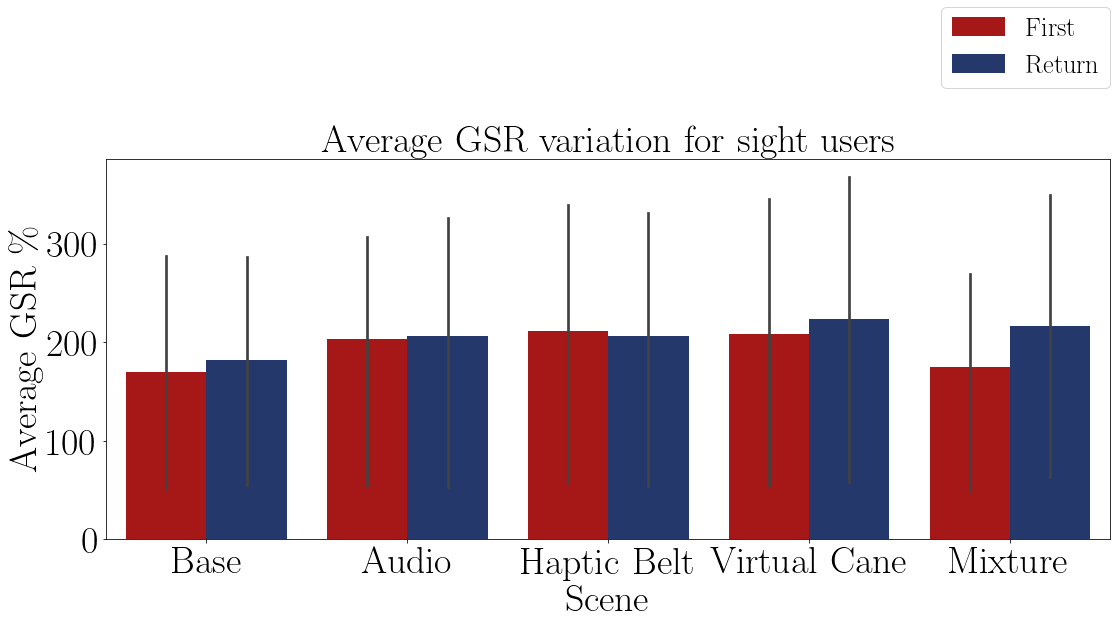
\includegraphics[width = 0.8\linewidth]{Resultados/GSR/Figuras/png/barplot_gsr_avg_scene_sight.png}
        %\resizebox{0.6\linewidth}{!}{
        %%% Creator: Matplotlib, PGF backend
%%
%% To include the figure in your LaTeX document, write
%%   \input{<filename>.pgf}
%%
%% Make sure the required packages are loaded in your preamble
%%   \usepackage{pgf}
%%
%% Figures using additional raster images can only be included by \input if
%% they are in the same directory as the main LaTeX file. For loading figures
%% from other directories you can use the `import` package
%%   \usepackage{import}
%%
%% and then include the figures with
%%   \import{<path to file>}{<filename>.pgf}
%%
%% Matplotlib used the following preamble
%%   \usepackage{fontspec}
%%
\begingroup%
\makeatletter%
\begin{pgfpicture}%
\pgfpathrectangle{\pgfpointorigin}{\pgfqpoint{15.281396in}{8.690562in}}%
\pgfusepath{use as bounding box, clip}%
\begin{pgfscope}%
\pgfsetbuttcap%
\pgfsetmiterjoin%
\pgfsetlinewidth{0.000000pt}%
\definecolor{currentstroke}{rgb}{1.000000,1.000000,1.000000}%
\pgfsetstrokecolor{currentstroke}%
\pgfsetstrokeopacity{0.000000}%
\pgfsetdash{}{0pt}%
\pgfpathmoveto{\pgfqpoint{0.000000in}{-0.000000in}}%
\pgfpathlineto{\pgfqpoint{15.281396in}{-0.000000in}}%
\pgfpathlineto{\pgfqpoint{15.281396in}{8.690562in}}%
\pgfpathlineto{\pgfqpoint{0.000000in}{8.690562in}}%
\pgfpathclose%
\pgfusepath{}%
\end{pgfscope}%
\begin{pgfscope}%
\pgfsetbuttcap%
\pgfsetmiterjoin%
\definecolor{currentfill}{rgb}{1.000000,1.000000,1.000000}%
\pgfsetfillcolor{currentfill}%
\pgfsetlinewidth{0.000000pt}%
\definecolor{currentstroke}{rgb}{0.000000,0.000000,0.000000}%
\pgfsetstrokecolor{currentstroke}%
\pgfsetstrokeopacity{0.000000}%
\pgfsetdash{}{0pt}%
\pgfpathmoveto{\pgfqpoint{1.231396in}{1.191562in}}%
\pgfpathlineto{\pgfqpoint{15.181396in}{1.191562in}}%
\pgfpathlineto{\pgfqpoint{15.181396in}{6.476562in}}%
\pgfpathlineto{\pgfqpoint{1.231396in}{6.476562in}}%
\pgfpathclose%
\pgfusepath{fill}%
\end{pgfscope}%
\begin{pgfscope}%
\pgfpathrectangle{\pgfqpoint{1.231396in}{1.191562in}}{\pgfqpoint{13.950000in}{5.285000in}}%
\pgfusepath{clip}%
\pgfsetbuttcap%
\pgfsetmiterjoin%
\definecolor{currentfill}{rgb}{0.651961,0.093137,0.093137}%
\pgfsetfillcolor{currentfill}%
\pgfsetlinewidth{0.000000pt}%
\definecolor{currentstroke}{rgb}{0.000000,0.000000,0.000000}%
\pgfsetstrokecolor{currentstroke}%
\pgfsetstrokeopacity{0.000000}%
\pgfsetdash{}{0pt}%
\pgfpathmoveto{\pgfqpoint{1.510396in}{1.191562in}}%
\pgfpathlineto{\pgfqpoint{2.626396in}{1.191562in}}%
\pgfpathlineto{\pgfqpoint{2.626396in}{3.511932in}}%
\pgfpathlineto{\pgfqpoint{1.510396in}{3.511932in}}%
\pgfpathclose%
\pgfusepath{fill}%
\end{pgfscope}%
\begin{pgfscope}%
\pgfpathrectangle{\pgfqpoint{1.231396in}{1.191562in}}{\pgfqpoint{13.950000in}{5.285000in}}%
\pgfusepath{clip}%
\pgfsetbuttcap%
\pgfsetmiterjoin%
\definecolor{currentfill}{rgb}{0.651961,0.093137,0.093137}%
\pgfsetfillcolor{currentfill}%
\pgfsetlinewidth{0.000000pt}%
\definecolor{currentstroke}{rgb}{0.000000,0.000000,0.000000}%
\pgfsetstrokecolor{currentstroke}%
\pgfsetstrokeopacity{0.000000}%
\pgfsetdash{}{0pt}%
\pgfpathmoveto{\pgfqpoint{4.300396in}{1.191562in}}%
\pgfpathlineto{\pgfqpoint{5.416396in}{1.191562in}}%
\pgfpathlineto{\pgfqpoint{5.416396in}{3.969940in}}%
\pgfpathlineto{\pgfqpoint{4.300396in}{3.969940in}}%
\pgfpathclose%
\pgfusepath{fill}%
\end{pgfscope}%
\begin{pgfscope}%
\pgfpathrectangle{\pgfqpoint{1.231396in}{1.191562in}}{\pgfqpoint{13.950000in}{5.285000in}}%
\pgfusepath{clip}%
\pgfsetbuttcap%
\pgfsetmiterjoin%
\definecolor{currentfill}{rgb}{0.651961,0.093137,0.093137}%
\pgfsetfillcolor{currentfill}%
\pgfsetlinewidth{0.000000pt}%
\definecolor{currentstroke}{rgb}{0.000000,0.000000,0.000000}%
\pgfsetstrokecolor{currentstroke}%
\pgfsetstrokeopacity{0.000000}%
\pgfsetdash{}{0pt}%
\pgfpathmoveto{\pgfqpoint{7.090396in}{1.191562in}}%
\pgfpathlineto{\pgfqpoint{8.206396in}{1.191562in}}%
\pgfpathlineto{\pgfqpoint{8.206396in}{4.086914in}}%
\pgfpathlineto{\pgfqpoint{7.090396in}{4.086914in}}%
\pgfpathclose%
\pgfusepath{fill}%
\end{pgfscope}%
\begin{pgfscope}%
\pgfpathrectangle{\pgfqpoint{1.231396in}{1.191562in}}{\pgfqpoint{13.950000in}{5.285000in}}%
\pgfusepath{clip}%
\pgfsetbuttcap%
\pgfsetmiterjoin%
\definecolor{currentfill}{rgb}{0.651961,0.093137,0.093137}%
\pgfsetfillcolor{currentfill}%
\pgfsetlinewidth{0.000000pt}%
\definecolor{currentstroke}{rgb}{0.000000,0.000000,0.000000}%
\pgfsetstrokecolor{currentstroke}%
\pgfsetstrokeopacity{0.000000}%
\pgfsetdash{}{0pt}%
\pgfpathmoveto{\pgfqpoint{9.880396in}{1.191562in}}%
\pgfpathlineto{\pgfqpoint{10.996396in}{1.191562in}}%
\pgfpathlineto{\pgfqpoint{10.996396in}{4.043061in}}%
\pgfpathlineto{\pgfqpoint{9.880396in}{4.043061in}}%
\pgfpathclose%
\pgfusepath{fill}%
\end{pgfscope}%
\begin{pgfscope}%
\pgfpathrectangle{\pgfqpoint{1.231396in}{1.191562in}}{\pgfqpoint{13.950000in}{5.285000in}}%
\pgfusepath{clip}%
\pgfsetbuttcap%
\pgfsetmiterjoin%
\definecolor{currentfill}{rgb}{0.651961,0.093137,0.093137}%
\pgfsetfillcolor{currentfill}%
\pgfsetlinewidth{0.000000pt}%
\definecolor{currentstroke}{rgb}{0.000000,0.000000,0.000000}%
\pgfsetstrokecolor{currentstroke}%
\pgfsetstrokeopacity{0.000000}%
\pgfsetdash{}{0pt}%
\pgfpathmoveto{\pgfqpoint{12.670396in}{1.191562in}}%
\pgfpathlineto{\pgfqpoint{13.786396in}{1.191562in}}%
\pgfpathlineto{\pgfqpoint{13.786396in}{3.591458in}}%
\pgfpathlineto{\pgfqpoint{12.670396in}{3.591458in}}%
\pgfpathclose%
\pgfusepath{fill}%
\end{pgfscope}%
\begin{pgfscope}%
\pgfpathrectangle{\pgfqpoint{1.231396in}{1.191562in}}{\pgfqpoint{13.950000in}{5.285000in}}%
\pgfusepath{clip}%
\pgfsetbuttcap%
\pgfsetmiterjoin%
\definecolor{currentfill}{rgb}{0.144608,0.218137,0.424020}%
\pgfsetfillcolor{currentfill}%
\pgfsetlinewidth{0.000000pt}%
\definecolor{currentstroke}{rgb}{0.000000,0.000000,0.000000}%
\pgfsetstrokecolor{currentstroke}%
\pgfsetstrokeopacity{0.000000}%
\pgfsetdash{}{0pt}%
\pgfpathmoveto{\pgfqpoint{2.626396in}{1.191562in}}%
\pgfpathlineto{\pgfqpoint{3.742396in}{1.191562in}}%
\pgfpathlineto{\pgfqpoint{3.742396in}{3.690373in}}%
\pgfpathlineto{\pgfqpoint{2.626396in}{3.690373in}}%
\pgfpathclose%
\pgfusepath{fill}%
\end{pgfscope}%
\begin{pgfscope}%
\pgfpathrectangle{\pgfqpoint{1.231396in}{1.191562in}}{\pgfqpoint{13.950000in}{5.285000in}}%
\pgfusepath{clip}%
\pgfsetbuttcap%
\pgfsetmiterjoin%
\definecolor{currentfill}{rgb}{0.144608,0.218137,0.424020}%
\pgfsetfillcolor{currentfill}%
\pgfsetlinewidth{0.000000pt}%
\definecolor{currentstroke}{rgb}{0.000000,0.000000,0.000000}%
\pgfsetstrokecolor{currentstroke}%
\pgfsetstrokeopacity{0.000000}%
\pgfsetdash{}{0pt}%
\pgfpathmoveto{\pgfqpoint{5.416396in}{1.191562in}}%
\pgfpathlineto{\pgfqpoint{6.532396in}{1.191562in}}%
\pgfpathlineto{\pgfqpoint{6.532396in}{4.013591in}}%
\pgfpathlineto{\pgfqpoint{5.416396in}{4.013591in}}%
\pgfpathclose%
\pgfusepath{fill}%
\end{pgfscope}%
\begin{pgfscope}%
\pgfpathrectangle{\pgfqpoint{1.231396in}{1.191562in}}{\pgfqpoint{13.950000in}{5.285000in}}%
\pgfusepath{clip}%
\pgfsetbuttcap%
\pgfsetmiterjoin%
\definecolor{currentfill}{rgb}{0.144608,0.218137,0.424020}%
\pgfsetfillcolor{currentfill}%
\pgfsetlinewidth{0.000000pt}%
\definecolor{currentstroke}{rgb}{0.000000,0.000000,0.000000}%
\pgfsetstrokecolor{currentstroke}%
\pgfsetstrokeopacity{0.000000}%
\pgfsetdash{}{0pt}%
\pgfpathmoveto{\pgfqpoint{8.206396in}{1.191562in}}%
\pgfpathlineto{\pgfqpoint{9.322396in}{1.191562in}}%
\pgfpathlineto{\pgfqpoint{9.322396in}{4.019938in}}%
\pgfpathlineto{\pgfqpoint{8.206396in}{4.019938in}}%
\pgfpathclose%
\pgfusepath{fill}%
\end{pgfscope}%
\begin{pgfscope}%
\pgfpathrectangle{\pgfqpoint{1.231396in}{1.191562in}}{\pgfqpoint{13.950000in}{5.285000in}}%
\pgfusepath{clip}%
\pgfsetbuttcap%
\pgfsetmiterjoin%
\definecolor{currentfill}{rgb}{0.144608,0.218137,0.424020}%
\pgfsetfillcolor{currentfill}%
\pgfsetlinewidth{0.000000pt}%
\definecolor{currentstroke}{rgb}{0.000000,0.000000,0.000000}%
\pgfsetstrokecolor{currentstroke}%
\pgfsetstrokeopacity{0.000000}%
\pgfsetdash{}{0pt}%
\pgfpathmoveto{\pgfqpoint{10.996396in}{1.191562in}}%
\pgfpathlineto{\pgfqpoint{12.112396in}{1.191562in}}%
\pgfpathlineto{\pgfqpoint{12.112396in}{4.247047in}}%
\pgfpathlineto{\pgfqpoint{10.996396in}{4.247047in}}%
\pgfpathclose%
\pgfusepath{fill}%
\end{pgfscope}%
\begin{pgfscope}%
\pgfpathrectangle{\pgfqpoint{1.231396in}{1.191562in}}{\pgfqpoint{13.950000in}{5.285000in}}%
\pgfusepath{clip}%
\pgfsetbuttcap%
\pgfsetmiterjoin%
\definecolor{currentfill}{rgb}{0.144608,0.218137,0.424020}%
\pgfsetfillcolor{currentfill}%
\pgfsetlinewidth{0.000000pt}%
\definecolor{currentstroke}{rgb}{0.000000,0.000000,0.000000}%
\pgfsetstrokecolor{currentstroke}%
\pgfsetstrokeopacity{0.000000}%
\pgfsetdash{}{0pt}%
\pgfpathmoveto{\pgfqpoint{13.786396in}{1.191562in}}%
\pgfpathlineto{\pgfqpoint{14.902396in}{1.191562in}}%
\pgfpathlineto{\pgfqpoint{14.902396in}{4.160726in}}%
\pgfpathlineto{\pgfqpoint{13.786396in}{4.160726in}}%
\pgfpathclose%
\pgfusepath{fill}%
\end{pgfscope}%
\begin{pgfscope}%
\pgfsetbuttcap%
\pgfsetroundjoin%
\definecolor{currentfill}{rgb}{0.000000,0.000000,0.000000}%
\pgfsetfillcolor{currentfill}%
\pgfsetlinewidth{0.803000pt}%
\definecolor{currentstroke}{rgb}{0.000000,0.000000,0.000000}%
\pgfsetstrokecolor{currentstroke}%
\pgfsetdash{}{0pt}%
\pgfsys@defobject{currentmarker}{\pgfqpoint{0.000000in}{-0.048611in}}{\pgfqpoint{0.000000in}{0.000000in}}{%
\pgfpathmoveto{\pgfqpoint{0.000000in}{0.000000in}}%
\pgfpathlineto{\pgfqpoint{0.000000in}{-0.048611in}}%
\pgfusepath{stroke,fill}%
}%
\begin{pgfscope}%
\pgfsys@transformshift{2.626396in}{1.191562in}%
\pgfsys@useobject{currentmarker}{}%
\end{pgfscope}%
\end{pgfscope}%
\begin{pgfscope}%
\definecolor{textcolor}{rgb}{0.000000,0.000000,0.000000}%
\pgfsetstrokecolor{textcolor}%
\pgfsetfillcolor{textcolor}%
\pgftext[x=2.626396in,y=1.094339in,,top]{\color{textcolor}\rmfamily\fontsize{38.016000}{45.619200}\selectfont Base}%
\end{pgfscope}%
\begin{pgfscope}%
\pgfsetbuttcap%
\pgfsetroundjoin%
\definecolor{currentfill}{rgb}{0.000000,0.000000,0.000000}%
\pgfsetfillcolor{currentfill}%
\pgfsetlinewidth{0.803000pt}%
\definecolor{currentstroke}{rgb}{0.000000,0.000000,0.000000}%
\pgfsetstrokecolor{currentstroke}%
\pgfsetdash{}{0pt}%
\pgfsys@defobject{currentmarker}{\pgfqpoint{0.000000in}{-0.048611in}}{\pgfqpoint{0.000000in}{0.000000in}}{%
\pgfpathmoveto{\pgfqpoint{0.000000in}{0.000000in}}%
\pgfpathlineto{\pgfqpoint{0.000000in}{-0.048611in}}%
\pgfusepath{stroke,fill}%
}%
\begin{pgfscope}%
\pgfsys@transformshift{5.416396in}{1.191562in}%
\pgfsys@useobject{currentmarker}{}%
\end{pgfscope}%
\end{pgfscope}%
\begin{pgfscope}%
\definecolor{textcolor}{rgb}{0.000000,0.000000,0.000000}%
\pgfsetstrokecolor{textcolor}%
\pgfsetfillcolor{textcolor}%
\pgftext[x=5.416396in,y=1.094339in,,top]{\color{textcolor}\rmfamily\fontsize{38.016000}{45.619200}\selectfont Audio}%
\end{pgfscope}%
\begin{pgfscope}%
\pgfsetbuttcap%
\pgfsetroundjoin%
\definecolor{currentfill}{rgb}{0.000000,0.000000,0.000000}%
\pgfsetfillcolor{currentfill}%
\pgfsetlinewidth{0.803000pt}%
\definecolor{currentstroke}{rgb}{0.000000,0.000000,0.000000}%
\pgfsetstrokecolor{currentstroke}%
\pgfsetdash{}{0pt}%
\pgfsys@defobject{currentmarker}{\pgfqpoint{0.000000in}{-0.048611in}}{\pgfqpoint{0.000000in}{0.000000in}}{%
\pgfpathmoveto{\pgfqpoint{0.000000in}{0.000000in}}%
\pgfpathlineto{\pgfqpoint{0.000000in}{-0.048611in}}%
\pgfusepath{stroke,fill}%
}%
\begin{pgfscope}%
\pgfsys@transformshift{8.206396in}{1.191562in}%
\pgfsys@useobject{currentmarker}{}%
\end{pgfscope}%
\end{pgfscope}%
\begin{pgfscope}%
\definecolor{textcolor}{rgb}{0.000000,0.000000,0.000000}%
\pgfsetstrokecolor{textcolor}%
\pgfsetfillcolor{textcolor}%
\pgftext[x=8.206396in,y=1.094339in,,top]{\color{textcolor}\rmfamily\fontsize{38.016000}{45.619200}\selectfont Haptic Belt}%
\end{pgfscope}%
\begin{pgfscope}%
\pgfsetbuttcap%
\pgfsetroundjoin%
\definecolor{currentfill}{rgb}{0.000000,0.000000,0.000000}%
\pgfsetfillcolor{currentfill}%
\pgfsetlinewidth{0.803000pt}%
\definecolor{currentstroke}{rgb}{0.000000,0.000000,0.000000}%
\pgfsetstrokecolor{currentstroke}%
\pgfsetdash{}{0pt}%
\pgfsys@defobject{currentmarker}{\pgfqpoint{0.000000in}{-0.048611in}}{\pgfqpoint{0.000000in}{0.000000in}}{%
\pgfpathmoveto{\pgfqpoint{0.000000in}{0.000000in}}%
\pgfpathlineto{\pgfqpoint{0.000000in}{-0.048611in}}%
\pgfusepath{stroke,fill}%
}%
\begin{pgfscope}%
\pgfsys@transformshift{10.996396in}{1.191562in}%
\pgfsys@useobject{currentmarker}{}%
\end{pgfscope}%
\end{pgfscope}%
\begin{pgfscope}%
\definecolor{textcolor}{rgb}{0.000000,0.000000,0.000000}%
\pgfsetstrokecolor{textcolor}%
\pgfsetfillcolor{textcolor}%
\pgftext[x=10.996396in,y=1.094339in,,top]{\color{textcolor}\rmfamily\fontsize{38.016000}{45.619200}\selectfont Virtual Cane}%
\end{pgfscope}%
\begin{pgfscope}%
\pgfsetbuttcap%
\pgfsetroundjoin%
\definecolor{currentfill}{rgb}{0.000000,0.000000,0.000000}%
\pgfsetfillcolor{currentfill}%
\pgfsetlinewidth{0.803000pt}%
\definecolor{currentstroke}{rgb}{0.000000,0.000000,0.000000}%
\pgfsetstrokecolor{currentstroke}%
\pgfsetdash{}{0pt}%
\pgfsys@defobject{currentmarker}{\pgfqpoint{0.000000in}{-0.048611in}}{\pgfqpoint{0.000000in}{0.000000in}}{%
\pgfpathmoveto{\pgfqpoint{0.000000in}{0.000000in}}%
\pgfpathlineto{\pgfqpoint{0.000000in}{-0.048611in}}%
\pgfusepath{stroke,fill}%
}%
\begin{pgfscope}%
\pgfsys@transformshift{13.786396in}{1.191562in}%
\pgfsys@useobject{currentmarker}{}%
\end{pgfscope}%
\end{pgfscope}%
\begin{pgfscope}%
\definecolor{textcolor}{rgb}{0.000000,0.000000,0.000000}%
\pgfsetstrokecolor{textcolor}%
\pgfsetfillcolor{textcolor}%
\pgftext[x=13.786396in,y=1.094339in,,top]{\color{textcolor}\rmfamily\fontsize{38.016000}{45.619200}\selectfont Mixture}%
\end{pgfscope}%
\begin{pgfscope}%
\definecolor{textcolor}{rgb}{0.000000,0.000000,0.000000}%
\pgfsetstrokecolor{textcolor}%
\pgfsetfillcolor{textcolor}%
\pgftext[x=8.206396in,y=0.569392in,,top]{\color{textcolor}\rmfamily\fontsize{38.016000}{45.619200}\selectfont Scene}%
\end{pgfscope}%
\begin{pgfscope}%
\pgfsetbuttcap%
\pgfsetroundjoin%
\definecolor{currentfill}{rgb}{0.000000,0.000000,0.000000}%
\pgfsetfillcolor{currentfill}%
\pgfsetlinewidth{0.803000pt}%
\definecolor{currentstroke}{rgb}{0.000000,0.000000,0.000000}%
\pgfsetstrokecolor{currentstroke}%
\pgfsetdash{}{0pt}%
\pgfsys@defobject{currentmarker}{\pgfqpoint{-0.048611in}{0.000000in}}{\pgfqpoint{-0.000000in}{0.000000in}}{%
\pgfpathmoveto{\pgfqpoint{-0.000000in}{0.000000in}}%
\pgfpathlineto{\pgfqpoint{-0.048611in}{0.000000in}}%
\pgfusepath{stroke,fill}%
}%
\begin{pgfscope}%
\pgfsys@transformshift{1.231396in}{1.191562in}%
\pgfsys@useobject{currentmarker}{}%
\end{pgfscope}%
\end{pgfscope}%
\begin{pgfscope}%
\definecolor{textcolor}{rgb}{0.000000,0.000000,0.000000}%
\pgfsetstrokecolor{textcolor}%
\pgfsetfillcolor{textcolor}%
\pgftext[x=0.975695in, y=1.008346in, left, base]{\color{textcolor}\rmfamily\fontsize{38.016000}{45.619200}\selectfont \(\displaystyle {0}\)}%
\end{pgfscope}%
\begin{pgfscope}%
\pgfsetbuttcap%
\pgfsetroundjoin%
\definecolor{currentfill}{rgb}{0.000000,0.000000,0.000000}%
\pgfsetfillcolor{currentfill}%
\pgfsetlinewidth{0.803000pt}%
\definecolor{currentstroke}{rgb}{0.000000,0.000000,0.000000}%
\pgfsetstrokecolor{currentstroke}%
\pgfsetdash{}{0pt}%
\pgfsys@defobject{currentmarker}{\pgfqpoint{-0.048611in}{0.000000in}}{\pgfqpoint{-0.000000in}{0.000000in}}{%
\pgfpathmoveto{\pgfqpoint{-0.000000in}{0.000000in}}%
\pgfpathlineto{\pgfqpoint{-0.048611in}{0.000000in}}%
\pgfusepath{stroke,fill}%
}%
\begin{pgfscope}%
\pgfsys@transformshift{1.231396in}{2.560159in}%
\pgfsys@useobject{currentmarker}{}%
\end{pgfscope}%
\end{pgfscope}%
\begin{pgfscope}%
\definecolor{textcolor}{rgb}{0.000000,0.000000,0.000000}%
\pgfsetstrokecolor{textcolor}%
\pgfsetfillcolor{textcolor}%
\pgftext[x=0.658739in, y=2.376942in, left, base]{\color{textcolor}\rmfamily\fontsize{38.016000}{45.619200}\selectfont \(\displaystyle {100}\)}%
\end{pgfscope}%
\begin{pgfscope}%
\pgfsetbuttcap%
\pgfsetroundjoin%
\definecolor{currentfill}{rgb}{0.000000,0.000000,0.000000}%
\pgfsetfillcolor{currentfill}%
\pgfsetlinewidth{0.803000pt}%
\definecolor{currentstroke}{rgb}{0.000000,0.000000,0.000000}%
\pgfsetstrokecolor{currentstroke}%
\pgfsetdash{}{0pt}%
\pgfsys@defobject{currentmarker}{\pgfqpoint{-0.048611in}{0.000000in}}{\pgfqpoint{-0.000000in}{0.000000in}}{%
\pgfpathmoveto{\pgfqpoint{-0.000000in}{0.000000in}}%
\pgfpathlineto{\pgfqpoint{-0.048611in}{0.000000in}}%
\pgfusepath{stroke,fill}%
}%
\begin{pgfscope}%
\pgfsys@transformshift{1.231396in}{3.928755in}%
\pgfsys@useobject{currentmarker}{}%
\end{pgfscope}%
\end{pgfscope}%
\begin{pgfscope}%
\definecolor{textcolor}{rgb}{0.000000,0.000000,0.000000}%
\pgfsetstrokecolor{textcolor}%
\pgfsetfillcolor{textcolor}%
\pgftext[x=0.658739in, y=3.745539in, left, base]{\color{textcolor}\rmfamily\fontsize{38.016000}{45.619200}\selectfont \(\displaystyle {200}\)}%
\end{pgfscope}%
\begin{pgfscope}%
\pgfsetbuttcap%
\pgfsetroundjoin%
\definecolor{currentfill}{rgb}{0.000000,0.000000,0.000000}%
\pgfsetfillcolor{currentfill}%
\pgfsetlinewidth{0.803000pt}%
\definecolor{currentstroke}{rgb}{0.000000,0.000000,0.000000}%
\pgfsetstrokecolor{currentstroke}%
\pgfsetdash{}{0pt}%
\pgfsys@defobject{currentmarker}{\pgfqpoint{-0.048611in}{0.000000in}}{\pgfqpoint{-0.000000in}{0.000000in}}{%
\pgfpathmoveto{\pgfqpoint{-0.000000in}{0.000000in}}%
\pgfpathlineto{\pgfqpoint{-0.048611in}{0.000000in}}%
\pgfusepath{stroke,fill}%
}%
\begin{pgfscope}%
\pgfsys@transformshift{1.231396in}{5.297352in}%
\pgfsys@useobject{currentmarker}{}%
\end{pgfscope}%
\end{pgfscope}%
\begin{pgfscope}%
\definecolor{textcolor}{rgb}{0.000000,0.000000,0.000000}%
\pgfsetstrokecolor{textcolor}%
\pgfsetfillcolor{textcolor}%
\pgftext[x=0.658739in, y=5.114136in, left, base]{\color{textcolor}\rmfamily\fontsize{38.016000}{45.619200}\selectfont \(\displaystyle {300}\)}%
\end{pgfscope}%
\begin{pgfscope}%
\definecolor{textcolor}{rgb}{0.000000,0.000000,0.000000}%
\pgfsetstrokecolor{textcolor}%
\pgfsetfillcolor{textcolor}%
\pgftext[x=0.603184in,y=3.834062in,,bottom,rotate=90.000000]{\color{textcolor}\rmfamily\fontsize{38.016000}{45.619200}\selectfont Average GSR \%}%
\end{pgfscope}%
\begin{pgfscope}%
\pgfpathrectangle{\pgfqpoint{1.231396in}{1.191562in}}{\pgfqpoint{13.950000in}{5.285000in}}%
\pgfusepath{clip}%
\pgfsetrectcap%
\pgfsetroundjoin%
\pgfsetlinewidth{2.710125pt}%
\definecolor{currentstroke}{rgb}{0.260000,0.260000,0.260000}%
\pgfsetstrokecolor{currentstroke}%
\pgfsetdash{}{0pt}%
\pgfpathmoveto{\pgfqpoint{2.068396in}{1.897169in}}%
\pgfpathlineto{\pgfqpoint{2.068396in}{5.126695in}}%
\pgfusepath{stroke}%
\end{pgfscope}%
\begin{pgfscope}%
\pgfpathrectangle{\pgfqpoint{1.231396in}{1.191562in}}{\pgfqpoint{13.950000in}{5.285000in}}%
\pgfusepath{clip}%
\pgfsetrectcap%
\pgfsetroundjoin%
\pgfsetlinewidth{2.710125pt}%
\definecolor{currentstroke}{rgb}{0.260000,0.260000,0.260000}%
\pgfsetstrokecolor{currentstroke}%
\pgfsetdash{}{0pt}%
\pgfpathmoveto{\pgfqpoint{4.858396in}{1.943825in}}%
\pgfpathlineto{\pgfqpoint{4.858396in}{5.444463in}}%
\pgfusepath{stroke}%
\end{pgfscope}%
\begin{pgfscope}%
\pgfpathrectangle{\pgfqpoint{1.231396in}{1.191562in}}{\pgfqpoint{13.950000in}{5.285000in}}%
\pgfusepath{clip}%
\pgfsetrectcap%
\pgfsetroundjoin%
\pgfsetlinewidth{2.710125pt}%
\definecolor{currentstroke}{rgb}{0.260000,0.260000,0.260000}%
\pgfsetstrokecolor{currentstroke}%
\pgfsetdash{}{0pt}%
\pgfpathmoveto{\pgfqpoint{7.648396in}{1.981923in}}%
\pgfpathlineto{\pgfqpoint{7.648396in}{5.839132in}}%
\pgfusepath{stroke}%
\end{pgfscope}%
\begin{pgfscope}%
\pgfpathrectangle{\pgfqpoint{1.231396in}{1.191562in}}{\pgfqpoint{13.950000in}{5.285000in}}%
\pgfusepath{clip}%
\pgfsetrectcap%
\pgfsetroundjoin%
\pgfsetlinewidth{2.710125pt}%
\definecolor{currentstroke}{rgb}{0.260000,0.260000,0.260000}%
\pgfsetstrokecolor{currentstroke}%
\pgfsetdash{}{0pt}%
\pgfpathmoveto{\pgfqpoint{10.438396in}{1.938265in}}%
\pgfpathlineto{\pgfqpoint{10.438396in}{5.917850in}}%
\pgfusepath{stroke}%
\end{pgfscope}%
\begin{pgfscope}%
\pgfpathrectangle{\pgfqpoint{1.231396in}{1.191562in}}{\pgfqpoint{13.950000in}{5.285000in}}%
\pgfusepath{clip}%
\pgfsetrectcap%
\pgfsetroundjoin%
\pgfsetlinewidth{2.710125pt}%
\definecolor{currentstroke}{rgb}{0.260000,0.260000,0.260000}%
\pgfsetstrokecolor{currentstroke}%
\pgfsetdash{}{0pt}%
\pgfpathmoveto{\pgfqpoint{13.228396in}{1.861914in}}%
\pgfpathlineto{\pgfqpoint{13.228396in}{4.872615in}}%
\pgfusepath{stroke}%
\end{pgfscope}%
\begin{pgfscope}%
\pgfpathrectangle{\pgfqpoint{1.231396in}{1.191562in}}{\pgfqpoint{13.950000in}{5.285000in}}%
\pgfusepath{clip}%
\pgfsetrectcap%
\pgfsetroundjoin%
\pgfsetlinewidth{2.710125pt}%
\definecolor{currentstroke}{rgb}{0.260000,0.260000,0.260000}%
\pgfsetstrokecolor{currentstroke}%
\pgfsetdash{}{0pt}%
\pgfpathmoveto{\pgfqpoint{3.184396in}{1.941799in}}%
\pgfpathlineto{\pgfqpoint{3.184396in}{5.115308in}}%
\pgfusepath{stroke}%
\end{pgfscope}%
\begin{pgfscope}%
\pgfpathrectangle{\pgfqpoint{1.231396in}{1.191562in}}{\pgfqpoint{13.950000in}{5.285000in}}%
\pgfusepath{clip}%
\pgfsetrectcap%
\pgfsetroundjoin%
\pgfsetlinewidth{2.710125pt}%
\definecolor{currentstroke}{rgb}{0.260000,0.260000,0.260000}%
\pgfsetstrokecolor{currentstroke}%
\pgfsetdash{}{0pt}%
\pgfpathmoveto{\pgfqpoint{5.974396in}{1.924633in}}%
\pgfpathlineto{\pgfqpoint{5.974396in}{5.658833in}}%
\pgfusepath{stroke}%
\end{pgfscope}%
\begin{pgfscope}%
\pgfpathrectangle{\pgfqpoint{1.231396in}{1.191562in}}{\pgfqpoint{13.950000in}{5.285000in}}%
\pgfusepath{clip}%
\pgfsetrectcap%
\pgfsetroundjoin%
\pgfsetlinewidth{2.710125pt}%
\definecolor{currentstroke}{rgb}{0.260000,0.260000,0.260000}%
\pgfsetstrokecolor{currentstroke}%
\pgfsetdash{}{0pt}%
\pgfpathmoveto{\pgfqpoint{8.764396in}{1.935764in}}%
\pgfpathlineto{\pgfqpoint{8.764396in}{5.859791in}}%
\pgfusepath{stroke}%
\end{pgfscope}%
\begin{pgfscope}%
\pgfpathrectangle{\pgfqpoint{1.231396in}{1.191562in}}{\pgfqpoint{13.950000in}{5.285000in}}%
\pgfusepath{clip}%
\pgfsetrectcap%
\pgfsetroundjoin%
\pgfsetlinewidth{2.710125pt}%
\definecolor{currentstroke}{rgb}{0.260000,0.260000,0.260000}%
\pgfsetstrokecolor{currentstroke}%
\pgfsetdash{}{0pt}%
\pgfpathmoveto{\pgfqpoint{11.554396in}{1.819956in}}%
\pgfpathlineto{\pgfqpoint{11.554396in}{6.224895in}}%
\pgfusepath{stroke}%
\end{pgfscope}%
\begin{pgfscope}%
\pgfpathrectangle{\pgfqpoint{1.231396in}{1.191562in}}{\pgfqpoint{13.950000in}{5.285000in}}%
\pgfusepath{clip}%
\pgfsetrectcap%
\pgfsetroundjoin%
\pgfsetlinewidth{2.710125pt}%
\definecolor{currentstroke}{rgb}{0.260000,0.260000,0.260000}%
\pgfsetstrokecolor{currentstroke}%
\pgfsetdash{}{0pt}%
\pgfpathmoveto{\pgfqpoint{14.344396in}{2.061192in}}%
\pgfpathlineto{\pgfqpoint{14.344396in}{5.973347in}}%
\pgfusepath{stroke}%
\end{pgfscope}%
\begin{pgfscope}%
\pgfsetrectcap%
\pgfsetmiterjoin%
\pgfsetlinewidth{0.803000pt}%
\definecolor{currentstroke}{rgb}{0.000000,0.000000,0.000000}%
\pgfsetstrokecolor{currentstroke}%
\pgfsetdash{}{0pt}%
\pgfpathmoveto{\pgfqpoint{1.231396in}{1.191562in}}%
\pgfpathlineto{\pgfqpoint{1.231396in}{6.476562in}}%
\pgfusepath{stroke}%
\end{pgfscope}%
\begin{pgfscope}%
\pgfsetrectcap%
\pgfsetmiterjoin%
\pgfsetlinewidth{0.803000pt}%
\definecolor{currentstroke}{rgb}{0.000000,0.000000,0.000000}%
\pgfsetstrokecolor{currentstroke}%
\pgfsetdash{}{0pt}%
\pgfpathmoveto{\pgfqpoint{15.181396in}{1.191562in}}%
\pgfpathlineto{\pgfqpoint{15.181396in}{6.476562in}}%
\pgfusepath{stroke}%
\end{pgfscope}%
\begin{pgfscope}%
\pgfsetrectcap%
\pgfsetmiterjoin%
\pgfsetlinewidth{0.803000pt}%
\definecolor{currentstroke}{rgb}{0.000000,0.000000,0.000000}%
\pgfsetstrokecolor{currentstroke}%
\pgfsetdash{}{0pt}%
\pgfpathmoveto{\pgfqpoint{1.231396in}{1.191562in}}%
\pgfpathlineto{\pgfqpoint{15.181396in}{1.191562in}}%
\pgfusepath{stroke}%
\end{pgfscope}%
\begin{pgfscope}%
\pgfsetrectcap%
\pgfsetmiterjoin%
\pgfsetlinewidth{0.803000pt}%
\definecolor{currentstroke}{rgb}{0.000000,0.000000,0.000000}%
\pgfsetstrokecolor{currentstroke}%
\pgfsetdash{}{0pt}%
\pgfpathmoveto{\pgfqpoint{1.231396in}{6.476562in}}%
\pgfpathlineto{\pgfqpoint{15.181396in}{6.476562in}}%
\pgfusepath{stroke}%
\end{pgfscope}%
\begin{pgfscope}%
\definecolor{textcolor}{rgb}{0.000000,0.000000,0.000000}%
\pgfsetstrokecolor{textcolor}%
\pgfsetfillcolor{textcolor}%
\pgftext[x=8.206396in,y=6.584273in,,base]{\color{textcolor}\rmfamily\fontsize{38.016000}{45.619200}\selectfont Average GSR variation for sight users}%
\end{pgfscope}%
\begin{pgfscope}%
\pgfsetbuttcap%
\pgfsetmiterjoin%
\definecolor{currentfill}{rgb}{1.000000,1.000000,1.000000}%
\pgfsetfillcolor{currentfill}%
\pgfsetfillopacity{0.800000}%
\pgfsetlinewidth{1.003750pt}%
\definecolor{currentstroke}{rgb}{0.800000,0.800000,0.800000}%
\pgfsetstrokecolor{currentstroke}%
\pgfsetstrokeopacity{0.800000}%
\pgfsetdash{}{0pt}%
\pgfpathmoveto{\pgfqpoint{12.902196in}{7.457562in}}%
\pgfpathlineto{\pgfqpoint{15.108062in}{7.457562in}}%
\pgfpathquadraticcurveto{\pgfqpoint{15.181396in}{7.457562in}}{\pgfqpoint{15.181396in}{7.530896in}}%
\pgfpathlineto{\pgfqpoint{15.181396in}{8.517228in}}%
\pgfpathquadraticcurveto{\pgfqpoint{15.181396in}{8.590562in}}{\pgfqpoint{15.108062in}{8.590562in}}%
\pgfpathlineto{\pgfqpoint{12.902196in}{8.590562in}}%
\pgfpathquadraticcurveto{\pgfqpoint{12.828862in}{8.590562in}}{\pgfqpoint{12.828862in}{8.517228in}}%
\pgfpathlineto{\pgfqpoint{12.828862in}{7.530896in}}%
\pgfpathquadraticcurveto{\pgfqpoint{12.828862in}{7.457562in}}{\pgfqpoint{12.902196in}{7.457562in}}%
\pgfpathclose%
\pgfusepath{stroke,fill}%
\end{pgfscope}%
\begin{pgfscope}%
\pgfsetbuttcap%
\pgfsetmiterjoin%
\definecolor{currentfill}{rgb}{0.651961,0.093137,0.093137}%
\pgfsetfillcolor{currentfill}%
\pgfsetlinewidth{0.000000pt}%
\definecolor{currentstroke}{rgb}{0.000000,0.000000,0.000000}%
\pgfsetstrokecolor{currentstroke}%
\pgfsetstrokeopacity{0.000000}%
\pgfsetdash{}{0pt}%
\pgfpathmoveto{\pgfqpoint{12.975529in}{8.187228in}}%
\pgfpathlineto{\pgfqpoint{13.708862in}{8.187228in}}%
\pgfpathlineto{\pgfqpoint{13.708862in}{8.443895in}}%
\pgfpathlineto{\pgfqpoint{12.975529in}{8.443895in}}%
\pgfpathclose%
\pgfusepath{fill}%
\end{pgfscope}%
\begin{pgfscope}%
\definecolor{textcolor}{rgb}{0.000000,0.000000,0.000000}%
\pgfsetstrokecolor{textcolor}%
\pgfsetfillcolor{textcolor}%
\pgftext[x=14.002196in,y=8.187228in,left,base]{\color{textcolor}\rmfamily\fontsize{26.400000}{31.680000}\selectfont First}%
\end{pgfscope}%
\begin{pgfscope}%
\pgfsetbuttcap%
\pgfsetmiterjoin%
\definecolor{currentfill}{rgb}{0.144608,0.218137,0.424020}%
\pgfsetfillcolor{currentfill}%
\pgfsetlinewidth{0.000000pt}%
\definecolor{currentstroke}{rgb}{0.000000,0.000000,0.000000}%
\pgfsetstrokecolor{currentstroke}%
\pgfsetstrokeopacity{0.000000}%
\pgfsetdash{}{0pt}%
\pgfpathmoveto{\pgfqpoint{12.975529in}{7.675729in}}%
\pgfpathlineto{\pgfqpoint{13.708862in}{7.675729in}}%
\pgfpathlineto{\pgfqpoint{13.708862in}{7.932395in}}%
\pgfpathlineto{\pgfqpoint{12.975529in}{7.932395in}}%
\pgfpathclose%
\pgfusepath{fill}%
\end{pgfscope}%
\begin{pgfscope}%
\definecolor{textcolor}{rgb}{0.000000,0.000000,0.000000}%
\pgfsetstrokecolor{textcolor}%
\pgfsetfillcolor{textcolor}%
\pgftext[x=14.002196in,y=7.675729in,left,base]{\color{textcolor}\rmfamily\fontsize{26.400000}{31.680000}\selectfont Return}%
\end{pgfscope}%
\end{pgfpicture}%
\makeatother%
\endgroup%
    
        %}
        \caption{Bar plot of the average skin conductance of the sighted participants on each method.}
        \label{fig:barplot_gsr_scene_sight}
    \end{minipage}
\end{figure}

The Figure \ref{fig:boxplot_ecg_bpm_scene} shows a comparison between both groups

\begin{figure}[!htb]
    %\centering
    \begin{minipage}{.45\linewidth}
        \centering
        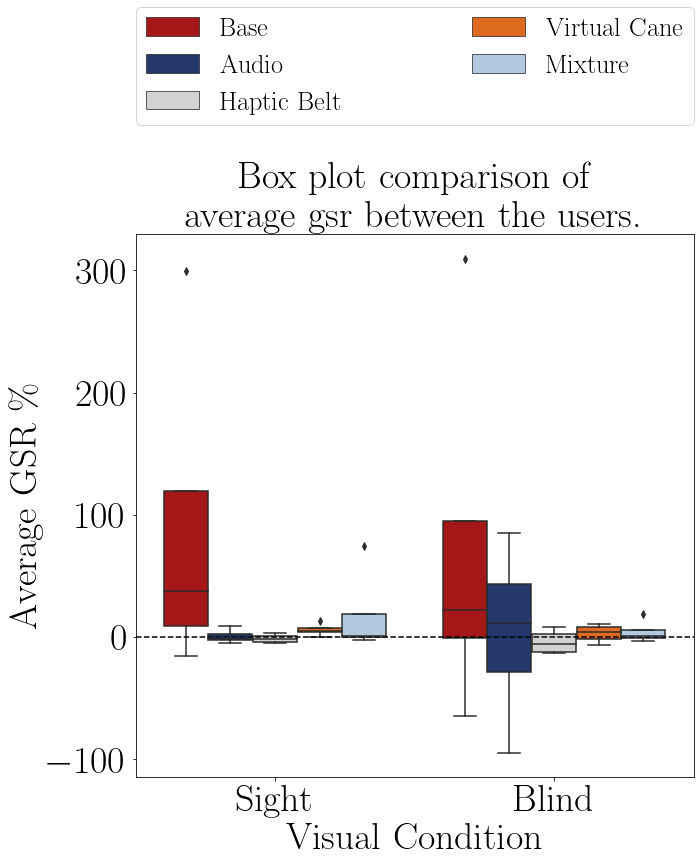
\includegraphics[width = \linewidth]{Resultados/GSR/Figuras/png/boxplot_gsr_avg_scene.png}
        \caption{Boxplot of the average skin conductace of the participants on each method.}
        \label{fig:boxplot_gsr_scene}
    \end{minipage}
    \begin{minipage}{.1\linewidth}
        \hfill
    \end{minipage}
    \begin{minipage}{.45\linewidth}
        \vspace{1.8cm}
        \centering
        %\hspace{-4cm}
        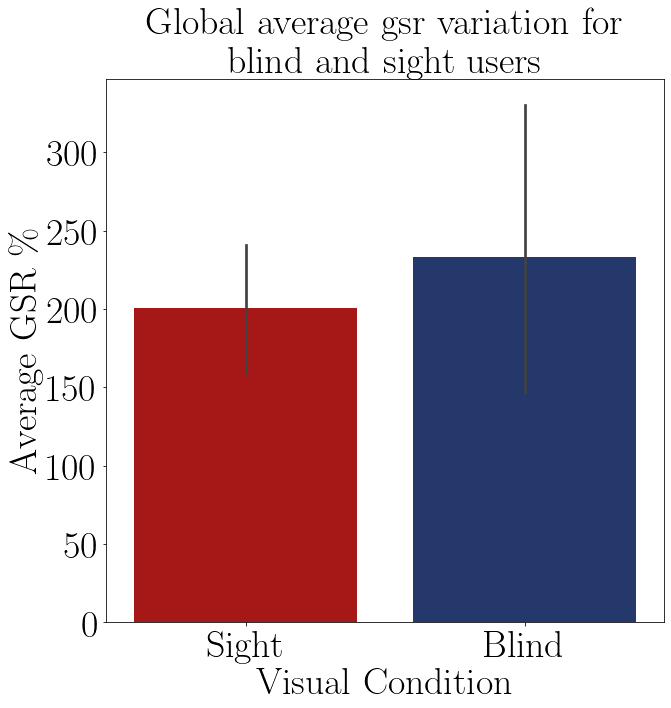
\includegraphics[width = \linewidth]{Resultados/GSR/Figuras/png/barplot_gsr_avg.png}
        \caption{Bar plot of the average GSR of of each group.}
        \label{fig:barplot_gsr_avg}
    \end{minipage}
\end{figure}

The Table \ref{tab:gsr_avg_table_def2} shows the variation of the heartbeat in each round of each group. It is also possible to notice the same increase noticed before.


\begin{table}[!htb]
\centering
\caption{Average GSR variation in relation to the baseline grouped by participant and visual Condition.}
\label{tab:gsr_avg_table_def2}
\begin{tabular}{lllrrrrrr}
\toprule
{} &     Base &    Audio & \begin{tabular}[c]{@{}l@{}}Haptic\\ Belt\end{tabular} & \begin{tabular}[c]{@{}l@{}}Virtual\\ Cane\end{tabular} &  Mixture \\
Visual Condition &          &          &                                                       &                                                        &          \\
\midrule
Blind            &  141.1\% &  127.3\% &                                               244.6\% &                                                307.2\% &  344.4\% \\
Sight            &  176.1\% &  204.6\% &                                               209.1\% &                                                215.8\% &  196.2\% \\
\bottomrule
\end{tabular}
\end{table}



The Shapiro–Wilk normality test on the Table \ref{tab:shapiro_gsr_avg} shows that only the "Audio" method is normally distributed for the "blind" sample while for the "sight" sample only the "Virtual Cane" is not normally distributed

According to the T-Test presented in the Table \ref{tab:ttest_gsr} there is no difference in the skin conductace  frequency variation between the sample groups.


\begin{table}[!htb]
    \begin{minipage}{.45\linewidth}
        
\centering
\caption{Shapiro test p-value for the gsr average for each method and visual condition}
\label{tab:shapiro_gsr_avg}
\begin{tabular}{lr}
\toprule
            Method &  Shapiro P-Value \\
\midrule
        Base blind &            0.002 \\
        Base sight &            0.187 \\
       Audio blind &            0.544 \\
       Audio sight &            0.046 \\
 Haptic Belt blind &            0.017 \\
 Haptic Belt sight &            0.155 \\
Virtual Cane blind &            0.004 \\
Virtual Cane sight &            0.275 \\
     Mixture blind &            0.011 \\
     Mixture sight &            0.376 \\
\bottomrule
\end{tabular}

    \end{minipage}
    \hfill
    \begin{minipage}{.45\linewidth}
        \vspace{-2.75cm}
        
\centering
\begin{tabular}{lr}
\toprule
      Method & T-Test P-Value \\
\midrule
        Base &        0.002** \\
       Audio &        0.022** \\
 Haptic Belt &          0.728 \\
Virtual Cane &          0.523 \\
     Mixture &          0.336 \\
\bottomrule
\end{tabular}

    \end{minipage}
\end{table}

The Table \ref{tab:repblocanova_gsr} shows the Anova test p-value of the skin conductance frequency of the "blind" sample between the guidance methods presented in the Table \ref{tab:gsr_avg_table}. The p-value indicates that there is at least one method that is statistically equal to one of the other methods.


\begin{table}[!htb]
\centering
\caption{Anova p-value for the GSR score on each method for blinded users.}
\label{tab:blocanova_gsr_avg}
\begin{tabular}{lrrrrr}
\toprule
               Source &  Squared sum &  DOF & Squared average &     F & \begin{tabular}[c]{@{}l@{}}P-Value \\ $(F_{0} > F)$\end{tabular} \\
\midrule
Participants (blocks) &  1918983.649 &    3 &      221654.067 & 9.552 &                                                                  \\
               Method &   886616.269 &    4 &      639661.216 & 3.310 &                                                          0.048** \\
   Experimental error &   803557.557 &   12 &       66963.130 &       &                                                                  \\
                Total &  3609157.475 &   39 &                 &       &                                                                  \\
\bottomrule
\end{tabular}
\end{table}



The Table \ref{tab:lsd_gsr} presents the conclusion of a pairwise Fisher LSD test of the blind skin conductance frequency variation between all the guidance methods. The results show that the "Virtual Cane" and the "Mixture" have different variations, but since they are not normally distributed this conclusion can not statistically be made.


\begin{table}[!htb]
\centering
\caption{Cross validation p-value for the GSR on each method for blinded users.}
\label{tab:lsd_gsr_avg}
\begin{tabular}{rclr}
\toprule
      \multicolumn{3}{c}{Method} &                                       Analysis \\
\midrule
              Base & $X$ & Audio &               $H_0 : \mu_{Base} = \mu_{Audio}$ \\
        Base & $X$ & Haptic Belt &         $H_0 : \mu_{Base} = \mu_{Haptic Belt}$ \\
       Base & $X$ & Virtual Cane &    $H_1 : \mu_{Base} \ne \mu_{Virtual Cane}**$ \\
            Base & $X$ & Mixture &         $H_1 : \mu_{Base} \ne \mu_{Mixture}**$ \\
       Audio & $X$ & Haptic Belt &    $H_1 : \mu_{Audio} \ne \mu_{Haptic Belt}**$ \\
      Audio & $X$ & Virtual Cane &   $H_1 : \mu_{Audio} \ne \mu_{Virtual Cane}**$ \\
           Audio & $X$ & Mixture &        $H_1 : \mu_{Audio} \ne \mu_{Mixture}**$ \\
Haptic Belt & $X$ & Virtual Cane & $H_0 : \mu_{Haptic Belt} = \mu_{Virtual Cane}$ \\
     Haptic Belt & $X$ & Mixture &      $H_0 : \mu_{Haptic Belt} = \mu_{Mixture}$ \\
    Virtual Cane & $X$ & Mixture &     $H_0 : \mu_{Virtual Cane} = \mu_{Mixture}$ \\
\bottomrule
\end{tabular}
\end{table}



According to the Anova test at Table \ref{tab:repblocanova_gsr} and the LSD test at \ref{tab:lsd_gsr} only the "Virtual Cane" and the "Mixture" method provoked a different reaction than the "Base" method, but since the Shapiro test at the Table \ref{tab:shapiro_gsr_avg} showed that they are not normally distributed, than this conclusion has no foundation.

\subsubsection{Analysis of the accumulated GSR}


%The Table \ref{tab:gsr_avg_table} presents the average skin conductance by each participant on each scenes and they are plotted in the Figures \ref{fig:barplot_gsr_scene_blind} and \ref{fig:barplot_gsr_scene_sight}. It is possible to see that in all of the methods there was an increase in the average skin conductance, meaning that the user was aroused and maybe an increase in the mental workload.


\begin{table}[!htb]
\centering
\caption{Accumulated GSR felled by the participants [$x10^4 \mu$S].}
\label{tab:gsr_sum_table}
\begin{tabular}{lllrrrrrr}
\toprule
    &       &        & Baseline &   Base &  Audio & \begin{tabular}[c]{@{}l@{}}Haptic\\ Belt\end{tabular} & \begin{tabular}[c]{@{}l@{}}Virtual\\ Cane\end{tabular} & Mixture \\
Part. & \begin{tabular}[c]{@{}l@{}}Visual\\ Condition\end{tabular} & Round &          &        &        &                                                       &                                                        &         \\
\midrule
001 & Sight & First &     8.45 &  21.35 &  18.76 &                                                 23.16 &                                                  30.53 &   14.53 \\
    &       & Return &          &  28.85 &  19.28 &                                                 19.90 &                                                  23.88 &   18.13 \\
001C & Blind & First &     0.16 &   1.06 &   1.51 &                                                  3.68 &                                                   4.08 &    4.62 \\
    &       & Return &          &   0.96 &   3.26 &                                                  4.87 &                                                   5.98 &    3.94 \\
002C & Blind & First &     0.07 &   2.35 &   0.35 &                                                  0.14 &                                                   0.12 &    0.13 \\
    &       & Return &          &   0.52 &   0.15 &                                                  0.23 &                                                   0.13 &    0.13 \\
003 & Sight & First &     0.30 &   0.15 &   0.50 &                                                  0.22 &                                                   0.18 &    0.14 \\
    &       & Return &          &   0.07 &   0.09 &                                                  0.14 &                                                   0.27 &    0.13 \\
003C & Blind & First &     0.16 &   0.72 &   0.53 &                                                  0.48 &                                                   1.46 &    1.16 \\
    &       & Return &          &   1.35 &   0.98 &                                                  0.66 &                                                   1.00 &    0.95 \\
004 & Sight & First &     1.26 &  12.41 &   9.77 &                                                 12.57 &                                                  13.42 &   12.47 \\
    &       & Return &          &  12.51 &   9.84 &                                                  4.12 &                                                  12.00 &   10.70 \\
004C & Blind & First &     0.60 &   3.82 &   4.13 &                                                  7.67 &                                                   1.96 &    2.75 \\
    &       & Return &          &   3.18 &   2.48 &                                                  3.11 &                                                   1.66 &    2.27 \\
005 & Sight & First &     0.23 &   2.99 &   2.67 &                                                  1.22 &                                                   1.78 &    0.77 \\
    &       & Return &          &   2.22 &   1.63 &                                                  1.46 &                                                   2.26 &    0.74 \\
\bottomrule
\end{tabular}
\end{table}



\begin{table}[!htb]
\centering
\caption{Accumulated GSR felled by the blind participants [$x10^4 \mu$S].}
\label{tab:gsr_sum_table_blind}
\begin{tabular}{llrrrrrr}
\toprule
     &        & Baseline &  Base & Audio & \begin{tabular}[c]{@{}l@{}}Haptic\\ Belt\end{tabular} & \begin{tabular}[c]{@{}l@{}}Virtual\\ Cane\end{tabular} & Mixture \\
Part. & Round &          &       &       &                                                       &                                                        &         \\
\midrule
001C & First &     0.16 &  1.06 &  1.51 &                                                  3.68 &                                                   4.08 &    4.62 \\
     & Return &          &  0.96 &  3.26 &                                                  4.87 &                                                   5.98 &    3.94 \\
002C & First &     0.07 &  2.35 &  0.35 &                                                  0.14 &                                                   0.12 &    0.13 \\
     & Return &          &  0.52 &  0.15 &                                                  0.23 &                                                   0.13 &    0.13 \\
003C & First &     0.16 &  0.72 &  0.53 &                                                  0.48 &                                                   1.46 &    1.16 \\
     & Return &          &  1.35 &  0.98 &                                                  0.66 &                                                   1.00 &    0.95 \\
004C & First &     0.60 &  3.82 &  4.13 &                                                  7.67 &                                                   1.96 &    2.75 \\
     & Return &          &  3.18 &  2.48 &                                                  3.11 &                                                   1.66 &    2.27 \\
\bottomrule
\end{tabular}
\end{table}



\begin{figure}[!htb]
    \centering
    \begin{minipage}{\textwidth}
        \centering
        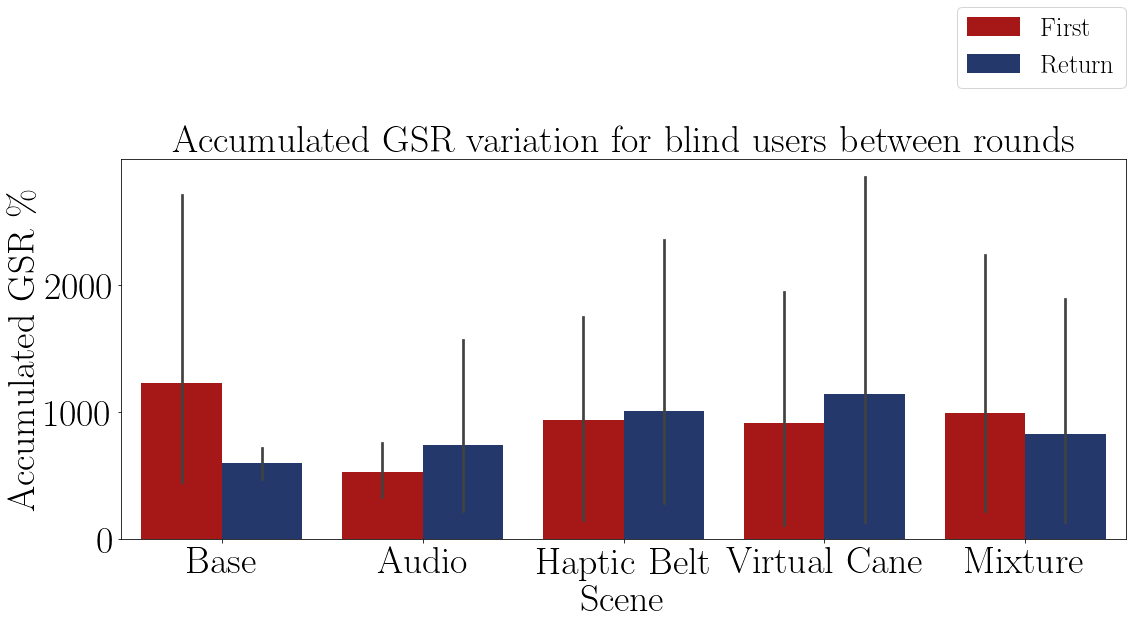
\includegraphics[width = 0.8\linewidth]{Resultados/GSR/Figuras/png/barplot_gsr_sum_scene_blind.png}
        %\resizebox{0.8\linewidth}{!}{
        %%% Creator: Matplotlib, PGF backend
%%
%% To include the figure in your LaTeX document, write
%%   \input{<filename>.pgf}
%%
%% Make sure the required packages are loaded in your preamble
%%   \usepackage{pgf}
%%
%% Figures using additional raster images can only be included by \input if
%% they are in the same directory as the main LaTeX file. For loading figures
%% from other directories you can use the `import` package
%%   \usepackage{import}
%%
%% and then include the figures with
%%   \import{<path to file>}{<filename>.pgf}
%%
%% Matplotlib used the following preamble
%%   \usepackage{fontspec}
%%
\begingroup%
\makeatletter%
\begin{pgfpicture}%
\pgfpathrectangle{\pgfpointorigin}{\pgfqpoint{15.369508in}{8.690562in}}%
\pgfusepath{use as bounding box, clip}%
\begin{pgfscope}%
\pgfsetbuttcap%
\pgfsetmiterjoin%
\pgfsetlinewidth{0.000000pt}%
\definecolor{currentstroke}{rgb}{1.000000,1.000000,1.000000}%
\pgfsetstrokecolor{currentstroke}%
\pgfsetstrokeopacity{0.000000}%
\pgfsetdash{}{0pt}%
\pgfpathmoveto{\pgfqpoint{0.000000in}{-0.000000in}}%
\pgfpathlineto{\pgfqpoint{15.369508in}{-0.000000in}}%
\pgfpathlineto{\pgfqpoint{15.369508in}{8.690562in}}%
\pgfpathlineto{\pgfqpoint{0.000000in}{8.690562in}}%
\pgfpathclose%
\pgfusepath{}%
\end{pgfscope}%
\begin{pgfscope}%
\pgfsetbuttcap%
\pgfsetmiterjoin%
\definecolor{currentfill}{rgb}{1.000000,1.000000,1.000000}%
\pgfsetfillcolor{currentfill}%
\pgfsetlinewidth{0.000000pt}%
\definecolor{currentstroke}{rgb}{0.000000,0.000000,0.000000}%
\pgfsetstrokecolor{currentstroke}%
\pgfsetstrokeopacity{0.000000}%
\pgfsetdash{}{0pt}%
\pgfpathmoveto{\pgfqpoint{1.319508in}{1.191562in}}%
\pgfpathlineto{\pgfqpoint{15.269508in}{1.191562in}}%
\pgfpathlineto{\pgfqpoint{15.269508in}{6.476562in}}%
\pgfpathlineto{\pgfqpoint{1.319508in}{6.476562in}}%
\pgfpathclose%
\pgfusepath{fill}%
\end{pgfscope}%
\begin{pgfscope}%
\pgfpathrectangle{\pgfqpoint{1.319508in}{1.191562in}}{\pgfqpoint{13.950000in}{5.285000in}}%
\pgfusepath{clip}%
\pgfsetbuttcap%
\pgfsetmiterjoin%
\definecolor{currentfill}{rgb}{0.651961,0.093137,0.093137}%
\pgfsetfillcolor{currentfill}%
\pgfsetlinewidth{0.000000pt}%
\definecolor{currentstroke}{rgb}{0.000000,0.000000,0.000000}%
\pgfsetstrokecolor{currentstroke}%
\pgfsetstrokeopacity{0.000000}%
\pgfsetdash{}{0pt}%
\pgfpathmoveto{\pgfqpoint{1.598508in}{5.432025in}}%
\pgfpathlineto{\pgfqpoint{2.714508in}{5.432025in}}%
\pgfpathlineto{\pgfqpoint{2.714508in}{4.583309in}}%
\pgfpathlineto{\pgfqpoint{1.598508in}{4.583309in}}%
\pgfpathclose%
\pgfusepath{fill}%
\end{pgfscope}%
\begin{pgfscope}%
\pgfpathrectangle{\pgfqpoint{1.319508in}{1.191562in}}{\pgfqpoint{13.950000in}{5.285000in}}%
\pgfusepath{clip}%
\pgfsetbuttcap%
\pgfsetmiterjoin%
\definecolor{currentfill}{rgb}{0.651961,0.093137,0.093137}%
\pgfsetfillcolor{currentfill}%
\pgfsetlinewidth{0.000000pt}%
\definecolor{currentstroke}{rgb}{0.000000,0.000000,0.000000}%
\pgfsetstrokecolor{currentstroke}%
\pgfsetstrokeopacity{0.000000}%
\pgfsetdash{}{0pt}%
\pgfpathmoveto{\pgfqpoint{4.388508in}{5.432025in}}%
\pgfpathlineto{\pgfqpoint{5.504508in}{5.432025in}}%
\pgfpathlineto{\pgfqpoint{5.504508in}{3.558465in}}%
\pgfpathlineto{\pgfqpoint{4.388508in}{3.558465in}}%
\pgfpathclose%
\pgfusepath{fill}%
\end{pgfscope}%
\begin{pgfscope}%
\pgfpathrectangle{\pgfqpoint{1.319508in}{1.191562in}}{\pgfqpoint{13.950000in}{5.285000in}}%
\pgfusepath{clip}%
\pgfsetbuttcap%
\pgfsetmiterjoin%
\definecolor{currentfill}{rgb}{0.651961,0.093137,0.093137}%
\pgfsetfillcolor{currentfill}%
\pgfsetlinewidth{0.000000pt}%
\definecolor{currentstroke}{rgb}{0.000000,0.000000,0.000000}%
\pgfsetstrokecolor{currentstroke}%
\pgfsetstrokeopacity{0.000000}%
\pgfsetdash{}{0pt}%
\pgfpathmoveto{\pgfqpoint{7.178508in}{5.432025in}}%
\pgfpathlineto{\pgfqpoint{8.294508in}{5.432025in}}%
\pgfpathlineto{\pgfqpoint{8.294508in}{4.476572in}}%
\pgfpathlineto{\pgfqpoint{7.178508in}{4.476572in}}%
\pgfpathclose%
\pgfusepath{fill}%
\end{pgfscope}%
\begin{pgfscope}%
\pgfpathrectangle{\pgfqpoint{1.319508in}{1.191562in}}{\pgfqpoint{13.950000in}{5.285000in}}%
\pgfusepath{clip}%
\pgfsetbuttcap%
\pgfsetmiterjoin%
\definecolor{currentfill}{rgb}{0.651961,0.093137,0.093137}%
\pgfsetfillcolor{currentfill}%
\pgfsetlinewidth{0.000000pt}%
\definecolor{currentstroke}{rgb}{0.000000,0.000000,0.000000}%
\pgfsetstrokecolor{currentstroke}%
\pgfsetstrokeopacity{0.000000}%
\pgfsetdash{}{0pt}%
\pgfpathmoveto{\pgfqpoint{9.968508in}{5.432025in}}%
\pgfpathlineto{\pgfqpoint{11.084508in}{5.432025in}}%
\pgfpathlineto{\pgfqpoint{11.084508in}{3.778608in}}%
\pgfpathlineto{\pgfqpoint{9.968508in}{3.778608in}}%
\pgfpathclose%
\pgfusepath{fill}%
\end{pgfscope}%
\begin{pgfscope}%
\pgfpathrectangle{\pgfqpoint{1.319508in}{1.191562in}}{\pgfqpoint{13.950000in}{5.285000in}}%
\pgfusepath{clip}%
\pgfsetbuttcap%
\pgfsetmiterjoin%
\definecolor{currentfill}{rgb}{0.651961,0.093137,0.093137}%
\pgfsetfillcolor{currentfill}%
\pgfsetlinewidth{0.000000pt}%
\definecolor{currentstroke}{rgb}{0.000000,0.000000,0.000000}%
\pgfsetstrokecolor{currentstroke}%
\pgfsetstrokeopacity{0.000000}%
\pgfsetdash{}{0pt}%
\pgfpathmoveto{\pgfqpoint{12.758508in}{5.432025in}}%
\pgfpathlineto{\pgfqpoint{13.874508in}{5.432025in}}%
\pgfpathlineto{\pgfqpoint{13.874508in}{4.339698in}}%
\pgfpathlineto{\pgfqpoint{12.758508in}{4.339698in}}%
\pgfpathclose%
\pgfusepath{fill}%
\end{pgfscope}%
\begin{pgfscope}%
\pgfpathrectangle{\pgfqpoint{1.319508in}{1.191562in}}{\pgfqpoint{13.950000in}{5.285000in}}%
\pgfusepath{clip}%
\pgfsetbuttcap%
\pgfsetmiterjoin%
\definecolor{currentfill}{rgb}{0.144608,0.218137,0.424020}%
\pgfsetfillcolor{currentfill}%
\pgfsetlinewidth{0.000000pt}%
\definecolor{currentstroke}{rgb}{0.000000,0.000000,0.000000}%
\pgfsetstrokecolor{currentstroke}%
\pgfsetstrokeopacity{0.000000}%
\pgfsetdash{}{0pt}%
\pgfpathmoveto{\pgfqpoint{2.714508in}{5.432025in}}%
\pgfpathlineto{\pgfqpoint{3.830508in}{5.432025in}}%
\pgfpathlineto{\pgfqpoint{3.830508in}{4.506389in}}%
\pgfpathlineto{\pgfqpoint{2.714508in}{4.506389in}}%
\pgfpathclose%
\pgfusepath{fill}%
\end{pgfscope}%
\begin{pgfscope}%
\pgfpathrectangle{\pgfqpoint{1.319508in}{1.191562in}}{\pgfqpoint{13.950000in}{5.285000in}}%
\pgfusepath{clip}%
\pgfsetbuttcap%
\pgfsetmiterjoin%
\definecolor{currentfill}{rgb}{0.144608,0.218137,0.424020}%
\pgfsetfillcolor{currentfill}%
\pgfsetlinewidth{0.000000pt}%
\definecolor{currentstroke}{rgb}{0.000000,0.000000,0.000000}%
\pgfsetstrokecolor{currentstroke}%
\pgfsetstrokeopacity{0.000000}%
\pgfsetdash{}{0pt}%
\pgfpathmoveto{\pgfqpoint{5.504508in}{5.432025in}}%
\pgfpathlineto{\pgfqpoint{6.620508in}{5.432025in}}%
\pgfpathlineto{\pgfqpoint{6.620508in}{3.808164in}}%
\pgfpathlineto{\pgfqpoint{5.504508in}{3.808164in}}%
\pgfpathclose%
\pgfusepath{fill}%
\end{pgfscope}%
\begin{pgfscope}%
\pgfpathrectangle{\pgfqpoint{1.319508in}{1.191562in}}{\pgfqpoint{13.950000in}{5.285000in}}%
\pgfusepath{clip}%
\pgfsetbuttcap%
\pgfsetmiterjoin%
\definecolor{currentfill}{rgb}{0.144608,0.218137,0.424020}%
\pgfsetfillcolor{currentfill}%
\pgfsetlinewidth{0.000000pt}%
\definecolor{currentstroke}{rgb}{0.000000,0.000000,0.000000}%
\pgfsetstrokecolor{currentstroke}%
\pgfsetstrokeopacity{0.000000}%
\pgfsetdash{}{0pt}%
\pgfpathmoveto{\pgfqpoint{8.294508in}{5.432025in}}%
\pgfpathlineto{\pgfqpoint{9.410508in}{5.432025in}}%
\pgfpathlineto{\pgfqpoint{9.410508in}{4.696413in}}%
\pgfpathlineto{\pgfqpoint{8.294508in}{4.696413in}}%
\pgfpathclose%
\pgfusepath{fill}%
\end{pgfscope}%
\begin{pgfscope}%
\pgfpathrectangle{\pgfqpoint{1.319508in}{1.191562in}}{\pgfqpoint{13.950000in}{5.285000in}}%
\pgfusepath{clip}%
\pgfsetbuttcap%
\pgfsetmiterjoin%
\definecolor{currentfill}{rgb}{0.144608,0.218137,0.424020}%
\pgfsetfillcolor{currentfill}%
\pgfsetlinewidth{0.000000pt}%
\definecolor{currentstroke}{rgb}{0.000000,0.000000,0.000000}%
\pgfsetstrokecolor{currentstroke}%
\pgfsetstrokeopacity{0.000000}%
\pgfsetdash{}{0pt}%
\pgfpathmoveto{\pgfqpoint{11.084508in}{5.432025in}}%
\pgfpathlineto{\pgfqpoint{12.200508in}{5.432025in}}%
\pgfpathlineto{\pgfqpoint{12.200508in}{4.423975in}}%
\pgfpathlineto{\pgfqpoint{11.084508in}{4.423975in}}%
\pgfpathclose%
\pgfusepath{fill}%
\end{pgfscope}%
\begin{pgfscope}%
\pgfpathrectangle{\pgfqpoint{1.319508in}{1.191562in}}{\pgfqpoint{13.950000in}{5.285000in}}%
\pgfusepath{clip}%
\pgfsetbuttcap%
\pgfsetmiterjoin%
\definecolor{currentfill}{rgb}{0.144608,0.218137,0.424020}%
\pgfsetfillcolor{currentfill}%
\pgfsetlinewidth{0.000000pt}%
\definecolor{currentstroke}{rgb}{0.000000,0.000000,0.000000}%
\pgfsetstrokecolor{currentstroke}%
\pgfsetstrokeopacity{0.000000}%
\pgfsetdash{}{0pt}%
\pgfpathmoveto{\pgfqpoint{13.874508in}{5.432025in}}%
\pgfpathlineto{\pgfqpoint{14.990508in}{5.432025in}}%
\pgfpathlineto{\pgfqpoint{14.990508in}{4.469000in}}%
\pgfpathlineto{\pgfqpoint{13.874508in}{4.469000in}}%
\pgfpathclose%
\pgfusepath{fill}%
\end{pgfscope}%
\begin{pgfscope}%
\pgfsetbuttcap%
\pgfsetroundjoin%
\definecolor{currentfill}{rgb}{0.000000,0.000000,0.000000}%
\pgfsetfillcolor{currentfill}%
\pgfsetlinewidth{0.803000pt}%
\definecolor{currentstroke}{rgb}{0.000000,0.000000,0.000000}%
\pgfsetstrokecolor{currentstroke}%
\pgfsetdash{}{0pt}%
\pgfsys@defobject{currentmarker}{\pgfqpoint{0.000000in}{-0.048611in}}{\pgfqpoint{0.000000in}{0.000000in}}{%
\pgfpathmoveto{\pgfqpoint{0.000000in}{0.000000in}}%
\pgfpathlineto{\pgfqpoint{0.000000in}{-0.048611in}}%
\pgfusepath{stroke,fill}%
}%
\begin{pgfscope}%
\pgfsys@transformshift{2.714508in}{1.191562in}%
\pgfsys@useobject{currentmarker}{}%
\end{pgfscope}%
\end{pgfscope}%
\begin{pgfscope}%
\definecolor{textcolor}{rgb}{0.000000,0.000000,0.000000}%
\pgfsetstrokecolor{textcolor}%
\pgfsetfillcolor{textcolor}%
\pgftext[x=2.714508in,y=1.094339in,,top]{\color{textcolor}\rmfamily\fontsize{38.016000}{45.619200}\selectfont Base}%
\end{pgfscope}%
\begin{pgfscope}%
\pgfsetbuttcap%
\pgfsetroundjoin%
\definecolor{currentfill}{rgb}{0.000000,0.000000,0.000000}%
\pgfsetfillcolor{currentfill}%
\pgfsetlinewidth{0.803000pt}%
\definecolor{currentstroke}{rgb}{0.000000,0.000000,0.000000}%
\pgfsetstrokecolor{currentstroke}%
\pgfsetdash{}{0pt}%
\pgfsys@defobject{currentmarker}{\pgfqpoint{0.000000in}{-0.048611in}}{\pgfqpoint{0.000000in}{0.000000in}}{%
\pgfpathmoveto{\pgfqpoint{0.000000in}{0.000000in}}%
\pgfpathlineto{\pgfqpoint{0.000000in}{-0.048611in}}%
\pgfusepath{stroke,fill}%
}%
\begin{pgfscope}%
\pgfsys@transformshift{5.504508in}{1.191562in}%
\pgfsys@useobject{currentmarker}{}%
\end{pgfscope}%
\end{pgfscope}%
\begin{pgfscope}%
\definecolor{textcolor}{rgb}{0.000000,0.000000,0.000000}%
\pgfsetstrokecolor{textcolor}%
\pgfsetfillcolor{textcolor}%
\pgftext[x=5.504508in,y=1.094339in,,top]{\color{textcolor}\rmfamily\fontsize{38.016000}{45.619200}\selectfont Audio}%
\end{pgfscope}%
\begin{pgfscope}%
\pgfsetbuttcap%
\pgfsetroundjoin%
\definecolor{currentfill}{rgb}{0.000000,0.000000,0.000000}%
\pgfsetfillcolor{currentfill}%
\pgfsetlinewidth{0.803000pt}%
\definecolor{currentstroke}{rgb}{0.000000,0.000000,0.000000}%
\pgfsetstrokecolor{currentstroke}%
\pgfsetdash{}{0pt}%
\pgfsys@defobject{currentmarker}{\pgfqpoint{0.000000in}{-0.048611in}}{\pgfqpoint{0.000000in}{0.000000in}}{%
\pgfpathmoveto{\pgfqpoint{0.000000in}{0.000000in}}%
\pgfpathlineto{\pgfqpoint{0.000000in}{-0.048611in}}%
\pgfusepath{stroke,fill}%
}%
\begin{pgfscope}%
\pgfsys@transformshift{8.294508in}{1.191562in}%
\pgfsys@useobject{currentmarker}{}%
\end{pgfscope}%
\end{pgfscope}%
\begin{pgfscope}%
\definecolor{textcolor}{rgb}{0.000000,0.000000,0.000000}%
\pgfsetstrokecolor{textcolor}%
\pgfsetfillcolor{textcolor}%
\pgftext[x=8.294508in,y=1.094339in,,top]{\color{textcolor}\rmfamily\fontsize{38.016000}{45.619200}\selectfont Haptic Belt}%
\end{pgfscope}%
\begin{pgfscope}%
\pgfsetbuttcap%
\pgfsetroundjoin%
\definecolor{currentfill}{rgb}{0.000000,0.000000,0.000000}%
\pgfsetfillcolor{currentfill}%
\pgfsetlinewidth{0.803000pt}%
\definecolor{currentstroke}{rgb}{0.000000,0.000000,0.000000}%
\pgfsetstrokecolor{currentstroke}%
\pgfsetdash{}{0pt}%
\pgfsys@defobject{currentmarker}{\pgfqpoint{0.000000in}{-0.048611in}}{\pgfqpoint{0.000000in}{0.000000in}}{%
\pgfpathmoveto{\pgfqpoint{0.000000in}{0.000000in}}%
\pgfpathlineto{\pgfqpoint{0.000000in}{-0.048611in}}%
\pgfusepath{stroke,fill}%
}%
\begin{pgfscope}%
\pgfsys@transformshift{11.084508in}{1.191562in}%
\pgfsys@useobject{currentmarker}{}%
\end{pgfscope}%
\end{pgfscope}%
\begin{pgfscope}%
\definecolor{textcolor}{rgb}{0.000000,0.000000,0.000000}%
\pgfsetstrokecolor{textcolor}%
\pgfsetfillcolor{textcolor}%
\pgftext[x=11.084508in,y=1.094339in,,top]{\color{textcolor}\rmfamily\fontsize{38.016000}{45.619200}\selectfont Virtual Cane}%
\end{pgfscope}%
\begin{pgfscope}%
\pgfsetbuttcap%
\pgfsetroundjoin%
\definecolor{currentfill}{rgb}{0.000000,0.000000,0.000000}%
\pgfsetfillcolor{currentfill}%
\pgfsetlinewidth{0.803000pt}%
\definecolor{currentstroke}{rgb}{0.000000,0.000000,0.000000}%
\pgfsetstrokecolor{currentstroke}%
\pgfsetdash{}{0pt}%
\pgfsys@defobject{currentmarker}{\pgfqpoint{0.000000in}{-0.048611in}}{\pgfqpoint{0.000000in}{0.000000in}}{%
\pgfpathmoveto{\pgfqpoint{0.000000in}{0.000000in}}%
\pgfpathlineto{\pgfqpoint{0.000000in}{-0.048611in}}%
\pgfusepath{stroke,fill}%
}%
\begin{pgfscope}%
\pgfsys@transformshift{13.874508in}{1.191562in}%
\pgfsys@useobject{currentmarker}{}%
\end{pgfscope}%
\end{pgfscope}%
\begin{pgfscope}%
\definecolor{textcolor}{rgb}{0.000000,0.000000,0.000000}%
\pgfsetstrokecolor{textcolor}%
\pgfsetfillcolor{textcolor}%
\pgftext[x=13.874508in,y=1.094339in,,top]{\color{textcolor}\rmfamily\fontsize{38.016000}{45.619200}\selectfont Mixture}%
\end{pgfscope}%
\begin{pgfscope}%
\definecolor{textcolor}{rgb}{0.000000,0.000000,0.000000}%
\pgfsetstrokecolor{textcolor}%
\pgfsetfillcolor{textcolor}%
\pgftext[x=8.294508in,y=0.569392in,,top]{\color{textcolor}\rmfamily\fontsize{38.016000}{45.619200}\selectfont Scene}%
\end{pgfscope}%
\begin{pgfscope}%
\pgfsetbuttcap%
\pgfsetroundjoin%
\definecolor{currentfill}{rgb}{0.000000,0.000000,0.000000}%
\pgfsetfillcolor{currentfill}%
\pgfsetlinewidth{0.803000pt}%
\definecolor{currentstroke}{rgb}{0.000000,0.000000,0.000000}%
\pgfsetstrokecolor{currentstroke}%
\pgfsetdash{}{0pt}%
\pgfsys@defobject{currentmarker}{\pgfqpoint{-0.048611in}{0.000000in}}{\pgfqpoint{-0.000000in}{0.000000in}}{%
\pgfpathmoveto{\pgfqpoint{-0.000000in}{0.000000in}}%
\pgfpathlineto{\pgfqpoint{-0.048611in}{0.000000in}}%
\pgfusepath{stroke,fill}%
}%
\begin{pgfscope}%
\pgfsys@transformshift{1.319508in}{1.767373in}%
\pgfsys@useobject{currentmarker}{}%
\end{pgfscope}%
\end{pgfscope}%
\begin{pgfscope}%
\definecolor{textcolor}{rgb}{0.000000,0.000000,0.000000}%
\pgfsetstrokecolor{textcolor}%
\pgfsetfillcolor{textcolor}%
\pgftext[x=0.636563in, y=1.584157in, left, base]{\color{textcolor}\rmfamily\fontsize{38.016000}{45.619200}\selectfont \(\displaystyle {\ensuremath{-}30}\)}%
\end{pgfscope}%
\begin{pgfscope}%
\pgfsetbuttcap%
\pgfsetroundjoin%
\definecolor{currentfill}{rgb}{0.000000,0.000000,0.000000}%
\pgfsetfillcolor{currentfill}%
\pgfsetlinewidth{0.803000pt}%
\definecolor{currentstroke}{rgb}{0.000000,0.000000,0.000000}%
\pgfsetstrokecolor{currentstroke}%
\pgfsetdash{}{0pt}%
\pgfsys@defobject{currentmarker}{\pgfqpoint{-0.048611in}{0.000000in}}{\pgfqpoint{-0.000000in}{0.000000in}}{%
\pgfpathmoveto{\pgfqpoint{-0.000000in}{0.000000in}}%
\pgfpathlineto{\pgfqpoint{-0.048611in}{0.000000in}}%
\pgfusepath{stroke,fill}%
}%
\begin{pgfscope}%
\pgfsys@transformshift{1.319508in}{2.988924in}%
\pgfsys@useobject{currentmarker}{}%
\end{pgfscope}%
\end{pgfscope}%
\begin{pgfscope}%
\definecolor{textcolor}{rgb}{0.000000,0.000000,0.000000}%
\pgfsetstrokecolor{textcolor}%
\pgfsetfillcolor{textcolor}%
\pgftext[x=0.636563in, y=2.805708in, left, base]{\color{textcolor}\rmfamily\fontsize{38.016000}{45.619200}\selectfont \(\displaystyle {\ensuremath{-}20}\)}%
\end{pgfscope}%
\begin{pgfscope}%
\pgfsetbuttcap%
\pgfsetroundjoin%
\definecolor{currentfill}{rgb}{0.000000,0.000000,0.000000}%
\pgfsetfillcolor{currentfill}%
\pgfsetlinewidth{0.803000pt}%
\definecolor{currentstroke}{rgb}{0.000000,0.000000,0.000000}%
\pgfsetstrokecolor{currentstroke}%
\pgfsetdash{}{0pt}%
\pgfsys@defobject{currentmarker}{\pgfqpoint{-0.048611in}{0.000000in}}{\pgfqpoint{-0.000000in}{0.000000in}}{%
\pgfpathmoveto{\pgfqpoint{-0.000000in}{0.000000in}}%
\pgfpathlineto{\pgfqpoint{-0.048611in}{0.000000in}}%
\pgfusepath{stroke,fill}%
}%
\begin{pgfscope}%
\pgfsys@transformshift{1.319508in}{4.210475in}%
\pgfsys@useobject{currentmarker}{}%
\end{pgfscope}%
\end{pgfscope}%
\begin{pgfscope}%
\definecolor{textcolor}{rgb}{0.000000,0.000000,0.000000}%
\pgfsetstrokecolor{textcolor}%
\pgfsetfillcolor{textcolor}%
\pgftext[x=0.636563in, y=4.027258in, left, base]{\color{textcolor}\rmfamily\fontsize{38.016000}{45.619200}\selectfont \(\displaystyle {\ensuremath{-}10}\)}%
\end{pgfscope}%
\begin{pgfscope}%
\pgfsetbuttcap%
\pgfsetroundjoin%
\definecolor{currentfill}{rgb}{0.000000,0.000000,0.000000}%
\pgfsetfillcolor{currentfill}%
\pgfsetlinewidth{0.803000pt}%
\definecolor{currentstroke}{rgb}{0.000000,0.000000,0.000000}%
\pgfsetstrokecolor{currentstroke}%
\pgfsetdash{}{0pt}%
\pgfsys@defobject{currentmarker}{\pgfqpoint{-0.048611in}{0.000000in}}{\pgfqpoint{-0.000000in}{0.000000in}}{%
\pgfpathmoveto{\pgfqpoint{-0.000000in}{0.000000in}}%
\pgfpathlineto{\pgfqpoint{-0.048611in}{0.000000in}}%
\pgfusepath{stroke,fill}%
}%
\begin{pgfscope}%
\pgfsys@transformshift{1.319508in}{5.432025in}%
\pgfsys@useobject{currentmarker}{}%
\end{pgfscope}%
\end{pgfscope}%
\begin{pgfscope}%
\definecolor{textcolor}{rgb}{0.000000,0.000000,0.000000}%
\pgfsetstrokecolor{textcolor}%
\pgfsetfillcolor{textcolor}%
\pgftext[x=1.063808in, y=5.248809in, left, base]{\color{textcolor}\rmfamily\fontsize{38.016000}{45.619200}\selectfont \(\displaystyle {0}\)}%
\end{pgfscope}%
\begin{pgfscope}%
\definecolor{textcolor}{rgb}{0.000000,0.000000,0.000000}%
\pgfsetstrokecolor{textcolor}%
\pgfsetfillcolor{textcolor}%
\pgftext[x=0.581008in,y=3.834062in,,bottom,rotate=90.000000]{\color{textcolor}\rmfamily\fontsize{38.016000}{45.619200}\selectfont Average BPM}%
\end{pgfscope}%
\begin{pgfscope}%
\pgfpathrectangle{\pgfqpoint{1.319508in}{1.191562in}}{\pgfqpoint{13.950000in}{5.285000in}}%
\pgfusepath{clip}%
\pgfsetrectcap%
\pgfsetroundjoin%
\pgfsetlinewidth{2.710125pt}%
\definecolor{currentstroke}{rgb}{0.260000,0.260000,0.260000}%
\pgfsetstrokecolor{currentstroke}%
\pgfsetdash{}{0pt}%
\pgfpathmoveto{\pgfqpoint{2.156508in}{2.751308in}}%
\pgfpathlineto{\pgfqpoint{2.156508in}{6.018483in}}%
\pgfusepath{stroke}%
\end{pgfscope}%
\begin{pgfscope}%
\pgfpathrectangle{\pgfqpoint{1.319508in}{1.191562in}}{\pgfqpoint{13.950000in}{5.285000in}}%
\pgfusepath{clip}%
\pgfsetrectcap%
\pgfsetroundjoin%
\pgfsetlinewidth{2.710125pt}%
\definecolor{currentstroke}{rgb}{0.260000,0.260000,0.260000}%
\pgfsetstrokecolor{currentstroke}%
\pgfsetdash{}{0pt}%
\pgfpathmoveto{\pgfqpoint{4.946508in}{1.431789in}}%
\pgfpathlineto{\pgfqpoint{4.946508in}{5.682086in}}%
\pgfusepath{stroke}%
\end{pgfscope}%
\begin{pgfscope}%
\pgfpathrectangle{\pgfqpoint{1.319508in}{1.191562in}}{\pgfqpoint{13.950000in}{5.285000in}}%
\pgfusepath{clip}%
\pgfsetrectcap%
\pgfsetroundjoin%
\pgfsetlinewidth{2.710125pt}%
\definecolor{currentstroke}{rgb}{0.260000,0.260000,0.260000}%
\pgfsetstrokecolor{currentstroke}%
\pgfsetdash{}{0pt}%
\pgfpathmoveto{\pgfqpoint{7.736508in}{2.678943in}}%
\pgfpathlineto{\pgfqpoint{7.736508in}{6.236334in}}%
\pgfusepath{stroke}%
\end{pgfscope}%
\begin{pgfscope}%
\pgfpathrectangle{\pgfqpoint{1.319508in}{1.191562in}}{\pgfqpoint{13.950000in}{5.285000in}}%
\pgfusepath{clip}%
\pgfsetrectcap%
\pgfsetroundjoin%
\pgfsetlinewidth{2.710125pt}%
\definecolor{currentstroke}{rgb}{0.260000,0.260000,0.260000}%
\pgfsetstrokecolor{currentstroke}%
\pgfsetdash{}{0pt}%
\pgfpathmoveto{\pgfqpoint{10.526508in}{2.047721in}}%
\pgfpathlineto{\pgfqpoint{10.526508in}{5.510294in}}%
\pgfusepath{stroke}%
\end{pgfscope}%
\begin{pgfscope}%
\pgfpathrectangle{\pgfqpoint{1.319508in}{1.191562in}}{\pgfqpoint{13.950000in}{5.285000in}}%
\pgfusepath{clip}%
\pgfsetrectcap%
\pgfsetroundjoin%
\pgfsetlinewidth{2.710125pt}%
\definecolor{currentstroke}{rgb}{0.260000,0.260000,0.260000}%
\pgfsetstrokecolor{currentstroke}%
\pgfsetdash{}{0pt}%
\pgfpathmoveto{\pgfqpoint{13.316508in}{3.163834in}}%
\pgfpathlineto{\pgfqpoint{13.316508in}{5.543100in}}%
\pgfusepath{stroke}%
\end{pgfscope}%
\begin{pgfscope}%
\pgfpathrectangle{\pgfqpoint{1.319508in}{1.191562in}}{\pgfqpoint{13.950000in}{5.285000in}}%
\pgfusepath{clip}%
\pgfsetrectcap%
\pgfsetroundjoin%
\pgfsetlinewidth{2.710125pt}%
\definecolor{currentstroke}{rgb}{0.260000,0.260000,0.260000}%
\pgfsetstrokecolor{currentstroke}%
\pgfsetdash{}{0pt}%
\pgfpathmoveto{\pgfqpoint{3.272508in}{3.222854in}}%
\pgfpathlineto{\pgfqpoint{3.272508in}{5.709606in}}%
\pgfusepath{stroke}%
\end{pgfscope}%
\begin{pgfscope}%
\pgfpathrectangle{\pgfqpoint{1.319508in}{1.191562in}}{\pgfqpoint{13.950000in}{5.285000in}}%
\pgfusepath{clip}%
\pgfsetrectcap%
\pgfsetroundjoin%
\pgfsetlinewidth{2.710125pt}%
\definecolor{currentstroke}{rgb}{0.260000,0.260000,0.260000}%
\pgfsetstrokecolor{currentstroke}%
\pgfsetdash{}{0pt}%
\pgfpathmoveto{\pgfqpoint{6.062508in}{1.933256in}}%
\pgfpathlineto{\pgfqpoint{6.062508in}{5.541904in}}%
\pgfusepath{stroke}%
\end{pgfscope}%
\begin{pgfscope}%
\pgfpathrectangle{\pgfqpoint{1.319508in}{1.191562in}}{\pgfqpoint{13.950000in}{5.285000in}}%
\pgfusepath{clip}%
\pgfsetrectcap%
\pgfsetroundjoin%
\pgfsetlinewidth{2.710125pt}%
\definecolor{currentstroke}{rgb}{0.260000,0.260000,0.260000}%
\pgfsetstrokecolor{currentstroke}%
\pgfsetdash{}{0pt}%
\pgfpathmoveto{\pgfqpoint{8.852508in}{3.694214in}}%
\pgfpathlineto{\pgfqpoint{8.852508in}{5.935485in}}%
\pgfusepath{stroke}%
\end{pgfscope}%
\begin{pgfscope}%
\pgfpathrectangle{\pgfqpoint{1.319508in}{1.191562in}}{\pgfqpoint{13.950000in}{5.285000in}}%
\pgfusepath{clip}%
\pgfsetrectcap%
\pgfsetroundjoin%
\pgfsetlinewidth{2.710125pt}%
\definecolor{currentstroke}{rgb}{0.260000,0.260000,0.260000}%
\pgfsetstrokecolor{currentstroke}%
\pgfsetdash{}{0pt}%
\pgfpathmoveto{\pgfqpoint{11.642508in}{3.336183in}}%
\pgfpathlineto{\pgfqpoint{11.642508in}{5.657013in}}%
\pgfusepath{stroke}%
\end{pgfscope}%
\begin{pgfscope}%
\pgfpathrectangle{\pgfqpoint{1.319508in}{1.191562in}}{\pgfqpoint{13.950000in}{5.285000in}}%
\pgfusepath{clip}%
\pgfsetrectcap%
\pgfsetroundjoin%
\pgfsetlinewidth{2.710125pt}%
\definecolor{currentstroke}{rgb}{0.260000,0.260000,0.260000}%
\pgfsetstrokecolor{currentstroke}%
\pgfsetdash{}{0pt}%
\pgfpathmoveto{\pgfqpoint{14.432508in}{3.718499in}}%
\pgfpathlineto{\pgfqpoint{14.432508in}{5.571045in}}%
\pgfusepath{stroke}%
\end{pgfscope}%
\begin{pgfscope}%
\pgfsetrectcap%
\pgfsetmiterjoin%
\pgfsetlinewidth{0.803000pt}%
\definecolor{currentstroke}{rgb}{0.000000,0.000000,0.000000}%
\pgfsetstrokecolor{currentstroke}%
\pgfsetdash{}{0pt}%
\pgfpathmoveto{\pgfqpoint{1.319508in}{1.191562in}}%
\pgfpathlineto{\pgfqpoint{1.319508in}{6.476562in}}%
\pgfusepath{stroke}%
\end{pgfscope}%
\begin{pgfscope}%
\pgfsetrectcap%
\pgfsetmiterjoin%
\pgfsetlinewidth{0.803000pt}%
\definecolor{currentstroke}{rgb}{0.000000,0.000000,0.000000}%
\pgfsetstrokecolor{currentstroke}%
\pgfsetdash{}{0pt}%
\pgfpathmoveto{\pgfqpoint{15.269508in}{1.191562in}}%
\pgfpathlineto{\pgfqpoint{15.269508in}{6.476562in}}%
\pgfusepath{stroke}%
\end{pgfscope}%
\begin{pgfscope}%
\pgfsetrectcap%
\pgfsetmiterjoin%
\pgfsetlinewidth{0.803000pt}%
\definecolor{currentstroke}{rgb}{0.000000,0.000000,0.000000}%
\pgfsetstrokecolor{currentstroke}%
\pgfsetdash{}{0pt}%
\pgfpathmoveto{\pgfqpoint{1.319508in}{1.191562in}}%
\pgfpathlineto{\pgfqpoint{15.269508in}{1.191562in}}%
\pgfusepath{stroke}%
\end{pgfscope}%
\begin{pgfscope}%
\pgfsetrectcap%
\pgfsetmiterjoin%
\pgfsetlinewidth{0.803000pt}%
\definecolor{currentstroke}{rgb}{0.000000,0.000000,0.000000}%
\pgfsetstrokecolor{currentstroke}%
\pgfsetdash{}{0pt}%
\pgfpathmoveto{\pgfqpoint{1.319508in}{6.476562in}}%
\pgfpathlineto{\pgfqpoint{15.269508in}{6.476562in}}%
\pgfusepath{stroke}%
\end{pgfscope}%
\begin{pgfscope}%
\definecolor{textcolor}{rgb}{0.000000,0.000000,0.000000}%
\pgfsetstrokecolor{textcolor}%
\pgfsetfillcolor{textcolor}%
\pgftext[x=8.294508in,y=6.584273in,,base]{\color{textcolor}\rmfamily\fontsize{38.016000}{45.619200}\selectfont Average BPM score variation for blind users between rounds}%
\end{pgfscope}%
\begin{pgfscope}%
\pgfsetbuttcap%
\pgfsetmiterjoin%
\definecolor{currentfill}{rgb}{1.000000,1.000000,1.000000}%
\pgfsetfillcolor{currentfill}%
\pgfsetfillopacity{0.800000}%
\pgfsetlinewidth{1.003750pt}%
\definecolor{currentstroke}{rgb}{0.800000,0.800000,0.800000}%
\pgfsetstrokecolor{currentstroke}%
\pgfsetstrokeopacity{0.800000}%
\pgfsetdash{}{0pt}%
\pgfpathmoveto{\pgfqpoint{12.990308in}{7.457562in}}%
\pgfpathlineto{\pgfqpoint{15.196175in}{7.457562in}}%
\pgfpathquadraticcurveto{\pgfqpoint{15.269508in}{7.457562in}}{\pgfqpoint{15.269508in}{7.530896in}}%
\pgfpathlineto{\pgfqpoint{15.269508in}{8.517228in}}%
\pgfpathquadraticcurveto{\pgfqpoint{15.269508in}{8.590562in}}{\pgfqpoint{15.196175in}{8.590562in}}%
\pgfpathlineto{\pgfqpoint{12.990308in}{8.590562in}}%
\pgfpathquadraticcurveto{\pgfqpoint{12.916975in}{8.590562in}}{\pgfqpoint{12.916975in}{8.517228in}}%
\pgfpathlineto{\pgfqpoint{12.916975in}{7.530896in}}%
\pgfpathquadraticcurveto{\pgfqpoint{12.916975in}{7.457562in}}{\pgfqpoint{12.990308in}{7.457562in}}%
\pgfpathclose%
\pgfusepath{stroke,fill}%
\end{pgfscope}%
\begin{pgfscope}%
\pgfsetbuttcap%
\pgfsetmiterjoin%
\definecolor{currentfill}{rgb}{0.651961,0.093137,0.093137}%
\pgfsetfillcolor{currentfill}%
\pgfsetlinewidth{0.000000pt}%
\definecolor{currentstroke}{rgb}{0.000000,0.000000,0.000000}%
\pgfsetstrokecolor{currentstroke}%
\pgfsetstrokeopacity{0.000000}%
\pgfsetdash{}{0pt}%
\pgfpathmoveto{\pgfqpoint{13.063642in}{8.187228in}}%
\pgfpathlineto{\pgfqpoint{13.796975in}{8.187228in}}%
\pgfpathlineto{\pgfqpoint{13.796975in}{8.443895in}}%
\pgfpathlineto{\pgfqpoint{13.063642in}{8.443895in}}%
\pgfpathclose%
\pgfusepath{fill}%
\end{pgfscope}%
\begin{pgfscope}%
\definecolor{textcolor}{rgb}{0.000000,0.000000,0.000000}%
\pgfsetstrokecolor{textcolor}%
\pgfsetfillcolor{textcolor}%
\pgftext[x=14.090308in,y=8.187228in,left,base]{\color{textcolor}\rmfamily\fontsize{26.400000}{31.680000}\selectfont First}%
\end{pgfscope}%
\begin{pgfscope}%
\pgfsetbuttcap%
\pgfsetmiterjoin%
\definecolor{currentfill}{rgb}{0.144608,0.218137,0.424020}%
\pgfsetfillcolor{currentfill}%
\pgfsetlinewidth{0.000000pt}%
\definecolor{currentstroke}{rgb}{0.000000,0.000000,0.000000}%
\pgfsetstrokecolor{currentstroke}%
\pgfsetstrokeopacity{0.000000}%
\pgfsetdash{}{0pt}%
\pgfpathmoveto{\pgfqpoint{13.063642in}{7.675729in}}%
\pgfpathlineto{\pgfqpoint{13.796975in}{7.675729in}}%
\pgfpathlineto{\pgfqpoint{13.796975in}{7.932395in}}%
\pgfpathlineto{\pgfqpoint{13.063642in}{7.932395in}}%
\pgfpathclose%
\pgfusepath{fill}%
\end{pgfscope}%
\begin{pgfscope}%
\definecolor{textcolor}{rgb}{0.000000,0.000000,0.000000}%
\pgfsetstrokecolor{textcolor}%
\pgfsetfillcolor{textcolor}%
\pgftext[x=14.090308in,y=7.675729in,left,base]{\color{textcolor}\rmfamily\fontsize{26.400000}{31.680000}\selectfont Return}%
\end{pgfscope}%
\end{pgfpicture}%
\makeatother%
\endgroup%

        %}
        \caption{Bar plot of the average skin conductance of the blind participants on each method.}
        \label{fig:barplot_gsr_scene_blind}
    \end{minipage}
    \begin{minipage}{\textwidth}
        \centering
        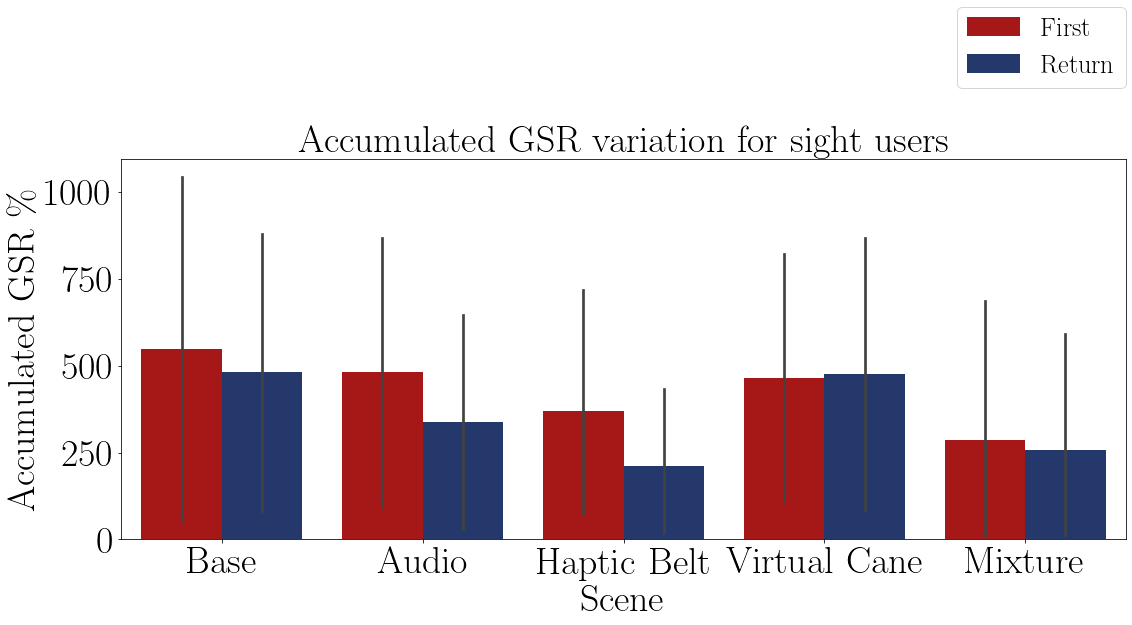
\includegraphics[width = 0.8\linewidth]{Resultados/GSR/Figuras/png/barplot_gsr_sum_scene_sight.png}
        %\resizebox{0.6\linewidth}{!}{
        %%% Creator: Matplotlib, PGF backend
%%
%% To include the figure in your LaTeX document, write
%%   \input{<filename>.pgf}
%%
%% Make sure the required packages are loaded in your preamble
%%   \usepackage{pgf}
%%
%% Figures using additional raster images can only be included by \input if
%% they are in the same directory as the main LaTeX file. For loading figures
%% from other directories you can use the `import` package
%%   \usepackage{import}
%%
%% and then include the figures with
%%   \import{<path to file>}{<filename>.pgf}
%%
%% Matplotlib used the following preamble
%%   \usepackage{fontspec}
%%
\begingroup%
\makeatletter%
\begin{pgfpicture}%
\pgfpathrectangle{\pgfpointorigin}{\pgfqpoint{15.281396in}{8.690562in}}%
\pgfusepath{use as bounding box, clip}%
\begin{pgfscope}%
\pgfsetbuttcap%
\pgfsetmiterjoin%
\pgfsetlinewidth{0.000000pt}%
\definecolor{currentstroke}{rgb}{1.000000,1.000000,1.000000}%
\pgfsetstrokecolor{currentstroke}%
\pgfsetstrokeopacity{0.000000}%
\pgfsetdash{}{0pt}%
\pgfpathmoveto{\pgfqpoint{0.000000in}{-0.000000in}}%
\pgfpathlineto{\pgfqpoint{15.281396in}{-0.000000in}}%
\pgfpathlineto{\pgfqpoint{15.281396in}{8.690562in}}%
\pgfpathlineto{\pgfqpoint{0.000000in}{8.690562in}}%
\pgfpathclose%
\pgfusepath{}%
\end{pgfscope}%
\begin{pgfscope}%
\pgfsetbuttcap%
\pgfsetmiterjoin%
\definecolor{currentfill}{rgb}{1.000000,1.000000,1.000000}%
\pgfsetfillcolor{currentfill}%
\pgfsetlinewidth{0.000000pt}%
\definecolor{currentstroke}{rgb}{0.000000,0.000000,0.000000}%
\pgfsetstrokecolor{currentstroke}%
\pgfsetstrokeopacity{0.000000}%
\pgfsetdash{}{0pt}%
\pgfpathmoveto{\pgfqpoint{1.231396in}{1.191562in}}%
\pgfpathlineto{\pgfqpoint{15.181396in}{1.191562in}}%
\pgfpathlineto{\pgfqpoint{15.181396in}{6.476562in}}%
\pgfpathlineto{\pgfqpoint{1.231396in}{6.476562in}}%
\pgfpathclose%
\pgfusepath{fill}%
\end{pgfscope}%
\begin{pgfscope}%
\pgfpathrectangle{\pgfqpoint{1.231396in}{1.191562in}}{\pgfqpoint{13.950000in}{5.285000in}}%
\pgfusepath{clip}%
\pgfsetbuttcap%
\pgfsetmiterjoin%
\definecolor{currentfill}{rgb}{0.651961,0.093137,0.093137}%
\pgfsetfillcolor{currentfill}%
\pgfsetlinewidth{0.000000pt}%
\definecolor{currentstroke}{rgb}{0.000000,0.000000,0.000000}%
\pgfsetstrokecolor{currentstroke}%
\pgfsetstrokeopacity{0.000000}%
\pgfsetdash{}{0pt}%
\pgfpathmoveto{\pgfqpoint{1.510396in}{1.191562in}}%
\pgfpathlineto{\pgfqpoint{2.626396in}{1.191562in}}%
\pgfpathlineto{\pgfqpoint{2.626396in}{3.511932in}}%
\pgfpathlineto{\pgfqpoint{1.510396in}{3.511932in}}%
\pgfpathclose%
\pgfusepath{fill}%
\end{pgfscope}%
\begin{pgfscope}%
\pgfpathrectangle{\pgfqpoint{1.231396in}{1.191562in}}{\pgfqpoint{13.950000in}{5.285000in}}%
\pgfusepath{clip}%
\pgfsetbuttcap%
\pgfsetmiterjoin%
\definecolor{currentfill}{rgb}{0.651961,0.093137,0.093137}%
\pgfsetfillcolor{currentfill}%
\pgfsetlinewidth{0.000000pt}%
\definecolor{currentstroke}{rgb}{0.000000,0.000000,0.000000}%
\pgfsetstrokecolor{currentstroke}%
\pgfsetstrokeopacity{0.000000}%
\pgfsetdash{}{0pt}%
\pgfpathmoveto{\pgfqpoint{4.300396in}{1.191562in}}%
\pgfpathlineto{\pgfqpoint{5.416396in}{1.191562in}}%
\pgfpathlineto{\pgfqpoint{5.416396in}{3.969940in}}%
\pgfpathlineto{\pgfqpoint{4.300396in}{3.969940in}}%
\pgfpathclose%
\pgfusepath{fill}%
\end{pgfscope}%
\begin{pgfscope}%
\pgfpathrectangle{\pgfqpoint{1.231396in}{1.191562in}}{\pgfqpoint{13.950000in}{5.285000in}}%
\pgfusepath{clip}%
\pgfsetbuttcap%
\pgfsetmiterjoin%
\definecolor{currentfill}{rgb}{0.651961,0.093137,0.093137}%
\pgfsetfillcolor{currentfill}%
\pgfsetlinewidth{0.000000pt}%
\definecolor{currentstroke}{rgb}{0.000000,0.000000,0.000000}%
\pgfsetstrokecolor{currentstroke}%
\pgfsetstrokeopacity{0.000000}%
\pgfsetdash{}{0pt}%
\pgfpathmoveto{\pgfqpoint{7.090396in}{1.191562in}}%
\pgfpathlineto{\pgfqpoint{8.206396in}{1.191562in}}%
\pgfpathlineto{\pgfqpoint{8.206396in}{4.086914in}}%
\pgfpathlineto{\pgfqpoint{7.090396in}{4.086914in}}%
\pgfpathclose%
\pgfusepath{fill}%
\end{pgfscope}%
\begin{pgfscope}%
\pgfpathrectangle{\pgfqpoint{1.231396in}{1.191562in}}{\pgfqpoint{13.950000in}{5.285000in}}%
\pgfusepath{clip}%
\pgfsetbuttcap%
\pgfsetmiterjoin%
\definecolor{currentfill}{rgb}{0.651961,0.093137,0.093137}%
\pgfsetfillcolor{currentfill}%
\pgfsetlinewidth{0.000000pt}%
\definecolor{currentstroke}{rgb}{0.000000,0.000000,0.000000}%
\pgfsetstrokecolor{currentstroke}%
\pgfsetstrokeopacity{0.000000}%
\pgfsetdash{}{0pt}%
\pgfpathmoveto{\pgfqpoint{9.880396in}{1.191562in}}%
\pgfpathlineto{\pgfqpoint{10.996396in}{1.191562in}}%
\pgfpathlineto{\pgfqpoint{10.996396in}{4.043061in}}%
\pgfpathlineto{\pgfqpoint{9.880396in}{4.043061in}}%
\pgfpathclose%
\pgfusepath{fill}%
\end{pgfscope}%
\begin{pgfscope}%
\pgfpathrectangle{\pgfqpoint{1.231396in}{1.191562in}}{\pgfqpoint{13.950000in}{5.285000in}}%
\pgfusepath{clip}%
\pgfsetbuttcap%
\pgfsetmiterjoin%
\definecolor{currentfill}{rgb}{0.651961,0.093137,0.093137}%
\pgfsetfillcolor{currentfill}%
\pgfsetlinewidth{0.000000pt}%
\definecolor{currentstroke}{rgb}{0.000000,0.000000,0.000000}%
\pgfsetstrokecolor{currentstroke}%
\pgfsetstrokeopacity{0.000000}%
\pgfsetdash{}{0pt}%
\pgfpathmoveto{\pgfqpoint{12.670396in}{1.191562in}}%
\pgfpathlineto{\pgfqpoint{13.786396in}{1.191562in}}%
\pgfpathlineto{\pgfqpoint{13.786396in}{3.591458in}}%
\pgfpathlineto{\pgfqpoint{12.670396in}{3.591458in}}%
\pgfpathclose%
\pgfusepath{fill}%
\end{pgfscope}%
\begin{pgfscope}%
\pgfpathrectangle{\pgfqpoint{1.231396in}{1.191562in}}{\pgfqpoint{13.950000in}{5.285000in}}%
\pgfusepath{clip}%
\pgfsetbuttcap%
\pgfsetmiterjoin%
\definecolor{currentfill}{rgb}{0.144608,0.218137,0.424020}%
\pgfsetfillcolor{currentfill}%
\pgfsetlinewidth{0.000000pt}%
\definecolor{currentstroke}{rgb}{0.000000,0.000000,0.000000}%
\pgfsetstrokecolor{currentstroke}%
\pgfsetstrokeopacity{0.000000}%
\pgfsetdash{}{0pt}%
\pgfpathmoveto{\pgfqpoint{2.626396in}{1.191562in}}%
\pgfpathlineto{\pgfqpoint{3.742396in}{1.191562in}}%
\pgfpathlineto{\pgfqpoint{3.742396in}{3.690373in}}%
\pgfpathlineto{\pgfqpoint{2.626396in}{3.690373in}}%
\pgfpathclose%
\pgfusepath{fill}%
\end{pgfscope}%
\begin{pgfscope}%
\pgfpathrectangle{\pgfqpoint{1.231396in}{1.191562in}}{\pgfqpoint{13.950000in}{5.285000in}}%
\pgfusepath{clip}%
\pgfsetbuttcap%
\pgfsetmiterjoin%
\definecolor{currentfill}{rgb}{0.144608,0.218137,0.424020}%
\pgfsetfillcolor{currentfill}%
\pgfsetlinewidth{0.000000pt}%
\definecolor{currentstroke}{rgb}{0.000000,0.000000,0.000000}%
\pgfsetstrokecolor{currentstroke}%
\pgfsetstrokeopacity{0.000000}%
\pgfsetdash{}{0pt}%
\pgfpathmoveto{\pgfqpoint{5.416396in}{1.191562in}}%
\pgfpathlineto{\pgfqpoint{6.532396in}{1.191562in}}%
\pgfpathlineto{\pgfqpoint{6.532396in}{4.013591in}}%
\pgfpathlineto{\pgfqpoint{5.416396in}{4.013591in}}%
\pgfpathclose%
\pgfusepath{fill}%
\end{pgfscope}%
\begin{pgfscope}%
\pgfpathrectangle{\pgfqpoint{1.231396in}{1.191562in}}{\pgfqpoint{13.950000in}{5.285000in}}%
\pgfusepath{clip}%
\pgfsetbuttcap%
\pgfsetmiterjoin%
\definecolor{currentfill}{rgb}{0.144608,0.218137,0.424020}%
\pgfsetfillcolor{currentfill}%
\pgfsetlinewidth{0.000000pt}%
\definecolor{currentstroke}{rgb}{0.000000,0.000000,0.000000}%
\pgfsetstrokecolor{currentstroke}%
\pgfsetstrokeopacity{0.000000}%
\pgfsetdash{}{0pt}%
\pgfpathmoveto{\pgfqpoint{8.206396in}{1.191562in}}%
\pgfpathlineto{\pgfqpoint{9.322396in}{1.191562in}}%
\pgfpathlineto{\pgfqpoint{9.322396in}{4.019938in}}%
\pgfpathlineto{\pgfqpoint{8.206396in}{4.019938in}}%
\pgfpathclose%
\pgfusepath{fill}%
\end{pgfscope}%
\begin{pgfscope}%
\pgfpathrectangle{\pgfqpoint{1.231396in}{1.191562in}}{\pgfqpoint{13.950000in}{5.285000in}}%
\pgfusepath{clip}%
\pgfsetbuttcap%
\pgfsetmiterjoin%
\definecolor{currentfill}{rgb}{0.144608,0.218137,0.424020}%
\pgfsetfillcolor{currentfill}%
\pgfsetlinewidth{0.000000pt}%
\definecolor{currentstroke}{rgb}{0.000000,0.000000,0.000000}%
\pgfsetstrokecolor{currentstroke}%
\pgfsetstrokeopacity{0.000000}%
\pgfsetdash{}{0pt}%
\pgfpathmoveto{\pgfqpoint{10.996396in}{1.191562in}}%
\pgfpathlineto{\pgfqpoint{12.112396in}{1.191562in}}%
\pgfpathlineto{\pgfqpoint{12.112396in}{4.247047in}}%
\pgfpathlineto{\pgfqpoint{10.996396in}{4.247047in}}%
\pgfpathclose%
\pgfusepath{fill}%
\end{pgfscope}%
\begin{pgfscope}%
\pgfpathrectangle{\pgfqpoint{1.231396in}{1.191562in}}{\pgfqpoint{13.950000in}{5.285000in}}%
\pgfusepath{clip}%
\pgfsetbuttcap%
\pgfsetmiterjoin%
\definecolor{currentfill}{rgb}{0.144608,0.218137,0.424020}%
\pgfsetfillcolor{currentfill}%
\pgfsetlinewidth{0.000000pt}%
\definecolor{currentstroke}{rgb}{0.000000,0.000000,0.000000}%
\pgfsetstrokecolor{currentstroke}%
\pgfsetstrokeopacity{0.000000}%
\pgfsetdash{}{0pt}%
\pgfpathmoveto{\pgfqpoint{13.786396in}{1.191562in}}%
\pgfpathlineto{\pgfqpoint{14.902396in}{1.191562in}}%
\pgfpathlineto{\pgfqpoint{14.902396in}{4.160726in}}%
\pgfpathlineto{\pgfqpoint{13.786396in}{4.160726in}}%
\pgfpathclose%
\pgfusepath{fill}%
\end{pgfscope}%
\begin{pgfscope}%
\pgfsetbuttcap%
\pgfsetroundjoin%
\definecolor{currentfill}{rgb}{0.000000,0.000000,0.000000}%
\pgfsetfillcolor{currentfill}%
\pgfsetlinewidth{0.803000pt}%
\definecolor{currentstroke}{rgb}{0.000000,0.000000,0.000000}%
\pgfsetstrokecolor{currentstroke}%
\pgfsetdash{}{0pt}%
\pgfsys@defobject{currentmarker}{\pgfqpoint{0.000000in}{-0.048611in}}{\pgfqpoint{0.000000in}{0.000000in}}{%
\pgfpathmoveto{\pgfqpoint{0.000000in}{0.000000in}}%
\pgfpathlineto{\pgfqpoint{0.000000in}{-0.048611in}}%
\pgfusepath{stroke,fill}%
}%
\begin{pgfscope}%
\pgfsys@transformshift{2.626396in}{1.191562in}%
\pgfsys@useobject{currentmarker}{}%
\end{pgfscope}%
\end{pgfscope}%
\begin{pgfscope}%
\definecolor{textcolor}{rgb}{0.000000,0.000000,0.000000}%
\pgfsetstrokecolor{textcolor}%
\pgfsetfillcolor{textcolor}%
\pgftext[x=2.626396in,y=1.094339in,,top]{\color{textcolor}\rmfamily\fontsize{38.016000}{45.619200}\selectfont Base}%
\end{pgfscope}%
\begin{pgfscope}%
\pgfsetbuttcap%
\pgfsetroundjoin%
\definecolor{currentfill}{rgb}{0.000000,0.000000,0.000000}%
\pgfsetfillcolor{currentfill}%
\pgfsetlinewidth{0.803000pt}%
\definecolor{currentstroke}{rgb}{0.000000,0.000000,0.000000}%
\pgfsetstrokecolor{currentstroke}%
\pgfsetdash{}{0pt}%
\pgfsys@defobject{currentmarker}{\pgfqpoint{0.000000in}{-0.048611in}}{\pgfqpoint{0.000000in}{0.000000in}}{%
\pgfpathmoveto{\pgfqpoint{0.000000in}{0.000000in}}%
\pgfpathlineto{\pgfqpoint{0.000000in}{-0.048611in}}%
\pgfusepath{stroke,fill}%
}%
\begin{pgfscope}%
\pgfsys@transformshift{5.416396in}{1.191562in}%
\pgfsys@useobject{currentmarker}{}%
\end{pgfscope}%
\end{pgfscope}%
\begin{pgfscope}%
\definecolor{textcolor}{rgb}{0.000000,0.000000,0.000000}%
\pgfsetstrokecolor{textcolor}%
\pgfsetfillcolor{textcolor}%
\pgftext[x=5.416396in,y=1.094339in,,top]{\color{textcolor}\rmfamily\fontsize{38.016000}{45.619200}\selectfont Audio}%
\end{pgfscope}%
\begin{pgfscope}%
\pgfsetbuttcap%
\pgfsetroundjoin%
\definecolor{currentfill}{rgb}{0.000000,0.000000,0.000000}%
\pgfsetfillcolor{currentfill}%
\pgfsetlinewidth{0.803000pt}%
\definecolor{currentstroke}{rgb}{0.000000,0.000000,0.000000}%
\pgfsetstrokecolor{currentstroke}%
\pgfsetdash{}{0pt}%
\pgfsys@defobject{currentmarker}{\pgfqpoint{0.000000in}{-0.048611in}}{\pgfqpoint{0.000000in}{0.000000in}}{%
\pgfpathmoveto{\pgfqpoint{0.000000in}{0.000000in}}%
\pgfpathlineto{\pgfqpoint{0.000000in}{-0.048611in}}%
\pgfusepath{stroke,fill}%
}%
\begin{pgfscope}%
\pgfsys@transformshift{8.206396in}{1.191562in}%
\pgfsys@useobject{currentmarker}{}%
\end{pgfscope}%
\end{pgfscope}%
\begin{pgfscope}%
\definecolor{textcolor}{rgb}{0.000000,0.000000,0.000000}%
\pgfsetstrokecolor{textcolor}%
\pgfsetfillcolor{textcolor}%
\pgftext[x=8.206396in,y=1.094339in,,top]{\color{textcolor}\rmfamily\fontsize{38.016000}{45.619200}\selectfont Haptic Belt}%
\end{pgfscope}%
\begin{pgfscope}%
\pgfsetbuttcap%
\pgfsetroundjoin%
\definecolor{currentfill}{rgb}{0.000000,0.000000,0.000000}%
\pgfsetfillcolor{currentfill}%
\pgfsetlinewidth{0.803000pt}%
\definecolor{currentstroke}{rgb}{0.000000,0.000000,0.000000}%
\pgfsetstrokecolor{currentstroke}%
\pgfsetdash{}{0pt}%
\pgfsys@defobject{currentmarker}{\pgfqpoint{0.000000in}{-0.048611in}}{\pgfqpoint{0.000000in}{0.000000in}}{%
\pgfpathmoveto{\pgfqpoint{0.000000in}{0.000000in}}%
\pgfpathlineto{\pgfqpoint{0.000000in}{-0.048611in}}%
\pgfusepath{stroke,fill}%
}%
\begin{pgfscope}%
\pgfsys@transformshift{10.996396in}{1.191562in}%
\pgfsys@useobject{currentmarker}{}%
\end{pgfscope}%
\end{pgfscope}%
\begin{pgfscope}%
\definecolor{textcolor}{rgb}{0.000000,0.000000,0.000000}%
\pgfsetstrokecolor{textcolor}%
\pgfsetfillcolor{textcolor}%
\pgftext[x=10.996396in,y=1.094339in,,top]{\color{textcolor}\rmfamily\fontsize{38.016000}{45.619200}\selectfont Virtual Cane}%
\end{pgfscope}%
\begin{pgfscope}%
\pgfsetbuttcap%
\pgfsetroundjoin%
\definecolor{currentfill}{rgb}{0.000000,0.000000,0.000000}%
\pgfsetfillcolor{currentfill}%
\pgfsetlinewidth{0.803000pt}%
\definecolor{currentstroke}{rgb}{0.000000,0.000000,0.000000}%
\pgfsetstrokecolor{currentstroke}%
\pgfsetdash{}{0pt}%
\pgfsys@defobject{currentmarker}{\pgfqpoint{0.000000in}{-0.048611in}}{\pgfqpoint{0.000000in}{0.000000in}}{%
\pgfpathmoveto{\pgfqpoint{0.000000in}{0.000000in}}%
\pgfpathlineto{\pgfqpoint{0.000000in}{-0.048611in}}%
\pgfusepath{stroke,fill}%
}%
\begin{pgfscope}%
\pgfsys@transformshift{13.786396in}{1.191562in}%
\pgfsys@useobject{currentmarker}{}%
\end{pgfscope}%
\end{pgfscope}%
\begin{pgfscope}%
\definecolor{textcolor}{rgb}{0.000000,0.000000,0.000000}%
\pgfsetstrokecolor{textcolor}%
\pgfsetfillcolor{textcolor}%
\pgftext[x=13.786396in,y=1.094339in,,top]{\color{textcolor}\rmfamily\fontsize{38.016000}{45.619200}\selectfont Mixture}%
\end{pgfscope}%
\begin{pgfscope}%
\definecolor{textcolor}{rgb}{0.000000,0.000000,0.000000}%
\pgfsetstrokecolor{textcolor}%
\pgfsetfillcolor{textcolor}%
\pgftext[x=8.206396in,y=0.569392in,,top]{\color{textcolor}\rmfamily\fontsize{38.016000}{45.619200}\selectfont Scene}%
\end{pgfscope}%
\begin{pgfscope}%
\pgfsetbuttcap%
\pgfsetroundjoin%
\definecolor{currentfill}{rgb}{0.000000,0.000000,0.000000}%
\pgfsetfillcolor{currentfill}%
\pgfsetlinewidth{0.803000pt}%
\definecolor{currentstroke}{rgb}{0.000000,0.000000,0.000000}%
\pgfsetstrokecolor{currentstroke}%
\pgfsetdash{}{0pt}%
\pgfsys@defobject{currentmarker}{\pgfqpoint{-0.048611in}{0.000000in}}{\pgfqpoint{-0.000000in}{0.000000in}}{%
\pgfpathmoveto{\pgfqpoint{-0.000000in}{0.000000in}}%
\pgfpathlineto{\pgfqpoint{-0.048611in}{0.000000in}}%
\pgfusepath{stroke,fill}%
}%
\begin{pgfscope}%
\pgfsys@transformshift{1.231396in}{1.191562in}%
\pgfsys@useobject{currentmarker}{}%
\end{pgfscope}%
\end{pgfscope}%
\begin{pgfscope}%
\definecolor{textcolor}{rgb}{0.000000,0.000000,0.000000}%
\pgfsetstrokecolor{textcolor}%
\pgfsetfillcolor{textcolor}%
\pgftext[x=0.975695in, y=1.008346in, left, base]{\color{textcolor}\rmfamily\fontsize{38.016000}{45.619200}\selectfont \(\displaystyle {0}\)}%
\end{pgfscope}%
\begin{pgfscope}%
\pgfsetbuttcap%
\pgfsetroundjoin%
\definecolor{currentfill}{rgb}{0.000000,0.000000,0.000000}%
\pgfsetfillcolor{currentfill}%
\pgfsetlinewidth{0.803000pt}%
\definecolor{currentstroke}{rgb}{0.000000,0.000000,0.000000}%
\pgfsetstrokecolor{currentstroke}%
\pgfsetdash{}{0pt}%
\pgfsys@defobject{currentmarker}{\pgfqpoint{-0.048611in}{0.000000in}}{\pgfqpoint{-0.000000in}{0.000000in}}{%
\pgfpathmoveto{\pgfqpoint{-0.000000in}{0.000000in}}%
\pgfpathlineto{\pgfqpoint{-0.048611in}{0.000000in}}%
\pgfusepath{stroke,fill}%
}%
\begin{pgfscope}%
\pgfsys@transformshift{1.231396in}{2.560159in}%
\pgfsys@useobject{currentmarker}{}%
\end{pgfscope}%
\end{pgfscope}%
\begin{pgfscope}%
\definecolor{textcolor}{rgb}{0.000000,0.000000,0.000000}%
\pgfsetstrokecolor{textcolor}%
\pgfsetfillcolor{textcolor}%
\pgftext[x=0.658739in, y=2.376942in, left, base]{\color{textcolor}\rmfamily\fontsize{38.016000}{45.619200}\selectfont \(\displaystyle {100}\)}%
\end{pgfscope}%
\begin{pgfscope}%
\pgfsetbuttcap%
\pgfsetroundjoin%
\definecolor{currentfill}{rgb}{0.000000,0.000000,0.000000}%
\pgfsetfillcolor{currentfill}%
\pgfsetlinewidth{0.803000pt}%
\definecolor{currentstroke}{rgb}{0.000000,0.000000,0.000000}%
\pgfsetstrokecolor{currentstroke}%
\pgfsetdash{}{0pt}%
\pgfsys@defobject{currentmarker}{\pgfqpoint{-0.048611in}{0.000000in}}{\pgfqpoint{-0.000000in}{0.000000in}}{%
\pgfpathmoveto{\pgfqpoint{-0.000000in}{0.000000in}}%
\pgfpathlineto{\pgfqpoint{-0.048611in}{0.000000in}}%
\pgfusepath{stroke,fill}%
}%
\begin{pgfscope}%
\pgfsys@transformshift{1.231396in}{3.928755in}%
\pgfsys@useobject{currentmarker}{}%
\end{pgfscope}%
\end{pgfscope}%
\begin{pgfscope}%
\definecolor{textcolor}{rgb}{0.000000,0.000000,0.000000}%
\pgfsetstrokecolor{textcolor}%
\pgfsetfillcolor{textcolor}%
\pgftext[x=0.658739in, y=3.745539in, left, base]{\color{textcolor}\rmfamily\fontsize{38.016000}{45.619200}\selectfont \(\displaystyle {200}\)}%
\end{pgfscope}%
\begin{pgfscope}%
\pgfsetbuttcap%
\pgfsetroundjoin%
\definecolor{currentfill}{rgb}{0.000000,0.000000,0.000000}%
\pgfsetfillcolor{currentfill}%
\pgfsetlinewidth{0.803000pt}%
\definecolor{currentstroke}{rgb}{0.000000,0.000000,0.000000}%
\pgfsetstrokecolor{currentstroke}%
\pgfsetdash{}{0pt}%
\pgfsys@defobject{currentmarker}{\pgfqpoint{-0.048611in}{0.000000in}}{\pgfqpoint{-0.000000in}{0.000000in}}{%
\pgfpathmoveto{\pgfqpoint{-0.000000in}{0.000000in}}%
\pgfpathlineto{\pgfqpoint{-0.048611in}{0.000000in}}%
\pgfusepath{stroke,fill}%
}%
\begin{pgfscope}%
\pgfsys@transformshift{1.231396in}{5.297352in}%
\pgfsys@useobject{currentmarker}{}%
\end{pgfscope}%
\end{pgfscope}%
\begin{pgfscope}%
\definecolor{textcolor}{rgb}{0.000000,0.000000,0.000000}%
\pgfsetstrokecolor{textcolor}%
\pgfsetfillcolor{textcolor}%
\pgftext[x=0.658739in, y=5.114136in, left, base]{\color{textcolor}\rmfamily\fontsize{38.016000}{45.619200}\selectfont \(\displaystyle {300}\)}%
\end{pgfscope}%
\begin{pgfscope}%
\definecolor{textcolor}{rgb}{0.000000,0.000000,0.000000}%
\pgfsetstrokecolor{textcolor}%
\pgfsetfillcolor{textcolor}%
\pgftext[x=0.603184in,y=3.834062in,,bottom,rotate=90.000000]{\color{textcolor}\rmfamily\fontsize{38.016000}{45.619200}\selectfont Average GSR \%}%
\end{pgfscope}%
\begin{pgfscope}%
\pgfpathrectangle{\pgfqpoint{1.231396in}{1.191562in}}{\pgfqpoint{13.950000in}{5.285000in}}%
\pgfusepath{clip}%
\pgfsetrectcap%
\pgfsetroundjoin%
\pgfsetlinewidth{2.710125pt}%
\definecolor{currentstroke}{rgb}{0.260000,0.260000,0.260000}%
\pgfsetstrokecolor{currentstroke}%
\pgfsetdash{}{0pt}%
\pgfpathmoveto{\pgfqpoint{2.068396in}{1.897169in}}%
\pgfpathlineto{\pgfqpoint{2.068396in}{5.126695in}}%
\pgfusepath{stroke}%
\end{pgfscope}%
\begin{pgfscope}%
\pgfpathrectangle{\pgfqpoint{1.231396in}{1.191562in}}{\pgfqpoint{13.950000in}{5.285000in}}%
\pgfusepath{clip}%
\pgfsetrectcap%
\pgfsetroundjoin%
\pgfsetlinewidth{2.710125pt}%
\definecolor{currentstroke}{rgb}{0.260000,0.260000,0.260000}%
\pgfsetstrokecolor{currentstroke}%
\pgfsetdash{}{0pt}%
\pgfpathmoveto{\pgfqpoint{4.858396in}{1.943825in}}%
\pgfpathlineto{\pgfqpoint{4.858396in}{5.444463in}}%
\pgfusepath{stroke}%
\end{pgfscope}%
\begin{pgfscope}%
\pgfpathrectangle{\pgfqpoint{1.231396in}{1.191562in}}{\pgfqpoint{13.950000in}{5.285000in}}%
\pgfusepath{clip}%
\pgfsetrectcap%
\pgfsetroundjoin%
\pgfsetlinewidth{2.710125pt}%
\definecolor{currentstroke}{rgb}{0.260000,0.260000,0.260000}%
\pgfsetstrokecolor{currentstroke}%
\pgfsetdash{}{0pt}%
\pgfpathmoveto{\pgfqpoint{7.648396in}{1.981923in}}%
\pgfpathlineto{\pgfqpoint{7.648396in}{5.839132in}}%
\pgfusepath{stroke}%
\end{pgfscope}%
\begin{pgfscope}%
\pgfpathrectangle{\pgfqpoint{1.231396in}{1.191562in}}{\pgfqpoint{13.950000in}{5.285000in}}%
\pgfusepath{clip}%
\pgfsetrectcap%
\pgfsetroundjoin%
\pgfsetlinewidth{2.710125pt}%
\definecolor{currentstroke}{rgb}{0.260000,0.260000,0.260000}%
\pgfsetstrokecolor{currentstroke}%
\pgfsetdash{}{0pt}%
\pgfpathmoveto{\pgfqpoint{10.438396in}{1.938265in}}%
\pgfpathlineto{\pgfqpoint{10.438396in}{5.917850in}}%
\pgfusepath{stroke}%
\end{pgfscope}%
\begin{pgfscope}%
\pgfpathrectangle{\pgfqpoint{1.231396in}{1.191562in}}{\pgfqpoint{13.950000in}{5.285000in}}%
\pgfusepath{clip}%
\pgfsetrectcap%
\pgfsetroundjoin%
\pgfsetlinewidth{2.710125pt}%
\definecolor{currentstroke}{rgb}{0.260000,0.260000,0.260000}%
\pgfsetstrokecolor{currentstroke}%
\pgfsetdash{}{0pt}%
\pgfpathmoveto{\pgfqpoint{13.228396in}{1.861914in}}%
\pgfpathlineto{\pgfqpoint{13.228396in}{4.872615in}}%
\pgfusepath{stroke}%
\end{pgfscope}%
\begin{pgfscope}%
\pgfpathrectangle{\pgfqpoint{1.231396in}{1.191562in}}{\pgfqpoint{13.950000in}{5.285000in}}%
\pgfusepath{clip}%
\pgfsetrectcap%
\pgfsetroundjoin%
\pgfsetlinewidth{2.710125pt}%
\definecolor{currentstroke}{rgb}{0.260000,0.260000,0.260000}%
\pgfsetstrokecolor{currentstroke}%
\pgfsetdash{}{0pt}%
\pgfpathmoveto{\pgfqpoint{3.184396in}{1.941799in}}%
\pgfpathlineto{\pgfqpoint{3.184396in}{5.115308in}}%
\pgfusepath{stroke}%
\end{pgfscope}%
\begin{pgfscope}%
\pgfpathrectangle{\pgfqpoint{1.231396in}{1.191562in}}{\pgfqpoint{13.950000in}{5.285000in}}%
\pgfusepath{clip}%
\pgfsetrectcap%
\pgfsetroundjoin%
\pgfsetlinewidth{2.710125pt}%
\definecolor{currentstroke}{rgb}{0.260000,0.260000,0.260000}%
\pgfsetstrokecolor{currentstroke}%
\pgfsetdash{}{0pt}%
\pgfpathmoveto{\pgfqpoint{5.974396in}{1.924633in}}%
\pgfpathlineto{\pgfqpoint{5.974396in}{5.658833in}}%
\pgfusepath{stroke}%
\end{pgfscope}%
\begin{pgfscope}%
\pgfpathrectangle{\pgfqpoint{1.231396in}{1.191562in}}{\pgfqpoint{13.950000in}{5.285000in}}%
\pgfusepath{clip}%
\pgfsetrectcap%
\pgfsetroundjoin%
\pgfsetlinewidth{2.710125pt}%
\definecolor{currentstroke}{rgb}{0.260000,0.260000,0.260000}%
\pgfsetstrokecolor{currentstroke}%
\pgfsetdash{}{0pt}%
\pgfpathmoveto{\pgfqpoint{8.764396in}{1.935764in}}%
\pgfpathlineto{\pgfqpoint{8.764396in}{5.859791in}}%
\pgfusepath{stroke}%
\end{pgfscope}%
\begin{pgfscope}%
\pgfpathrectangle{\pgfqpoint{1.231396in}{1.191562in}}{\pgfqpoint{13.950000in}{5.285000in}}%
\pgfusepath{clip}%
\pgfsetrectcap%
\pgfsetroundjoin%
\pgfsetlinewidth{2.710125pt}%
\definecolor{currentstroke}{rgb}{0.260000,0.260000,0.260000}%
\pgfsetstrokecolor{currentstroke}%
\pgfsetdash{}{0pt}%
\pgfpathmoveto{\pgfqpoint{11.554396in}{1.819956in}}%
\pgfpathlineto{\pgfqpoint{11.554396in}{6.224895in}}%
\pgfusepath{stroke}%
\end{pgfscope}%
\begin{pgfscope}%
\pgfpathrectangle{\pgfqpoint{1.231396in}{1.191562in}}{\pgfqpoint{13.950000in}{5.285000in}}%
\pgfusepath{clip}%
\pgfsetrectcap%
\pgfsetroundjoin%
\pgfsetlinewidth{2.710125pt}%
\definecolor{currentstroke}{rgb}{0.260000,0.260000,0.260000}%
\pgfsetstrokecolor{currentstroke}%
\pgfsetdash{}{0pt}%
\pgfpathmoveto{\pgfqpoint{14.344396in}{2.061192in}}%
\pgfpathlineto{\pgfqpoint{14.344396in}{5.973347in}}%
\pgfusepath{stroke}%
\end{pgfscope}%
\begin{pgfscope}%
\pgfsetrectcap%
\pgfsetmiterjoin%
\pgfsetlinewidth{0.803000pt}%
\definecolor{currentstroke}{rgb}{0.000000,0.000000,0.000000}%
\pgfsetstrokecolor{currentstroke}%
\pgfsetdash{}{0pt}%
\pgfpathmoveto{\pgfqpoint{1.231396in}{1.191562in}}%
\pgfpathlineto{\pgfqpoint{1.231396in}{6.476562in}}%
\pgfusepath{stroke}%
\end{pgfscope}%
\begin{pgfscope}%
\pgfsetrectcap%
\pgfsetmiterjoin%
\pgfsetlinewidth{0.803000pt}%
\definecolor{currentstroke}{rgb}{0.000000,0.000000,0.000000}%
\pgfsetstrokecolor{currentstroke}%
\pgfsetdash{}{0pt}%
\pgfpathmoveto{\pgfqpoint{15.181396in}{1.191562in}}%
\pgfpathlineto{\pgfqpoint{15.181396in}{6.476562in}}%
\pgfusepath{stroke}%
\end{pgfscope}%
\begin{pgfscope}%
\pgfsetrectcap%
\pgfsetmiterjoin%
\pgfsetlinewidth{0.803000pt}%
\definecolor{currentstroke}{rgb}{0.000000,0.000000,0.000000}%
\pgfsetstrokecolor{currentstroke}%
\pgfsetdash{}{0pt}%
\pgfpathmoveto{\pgfqpoint{1.231396in}{1.191562in}}%
\pgfpathlineto{\pgfqpoint{15.181396in}{1.191562in}}%
\pgfusepath{stroke}%
\end{pgfscope}%
\begin{pgfscope}%
\pgfsetrectcap%
\pgfsetmiterjoin%
\pgfsetlinewidth{0.803000pt}%
\definecolor{currentstroke}{rgb}{0.000000,0.000000,0.000000}%
\pgfsetstrokecolor{currentstroke}%
\pgfsetdash{}{0pt}%
\pgfpathmoveto{\pgfqpoint{1.231396in}{6.476562in}}%
\pgfpathlineto{\pgfqpoint{15.181396in}{6.476562in}}%
\pgfusepath{stroke}%
\end{pgfscope}%
\begin{pgfscope}%
\definecolor{textcolor}{rgb}{0.000000,0.000000,0.000000}%
\pgfsetstrokecolor{textcolor}%
\pgfsetfillcolor{textcolor}%
\pgftext[x=8.206396in,y=6.584273in,,base]{\color{textcolor}\rmfamily\fontsize{38.016000}{45.619200}\selectfont Average GSR variation for sight users}%
\end{pgfscope}%
\begin{pgfscope}%
\pgfsetbuttcap%
\pgfsetmiterjoin%
\definecolor{currentfill}{rgb}{1.000000,1.000000,1.000000}%
\pgfsetfillcolor{currentfill}%
\pgfsetfillopacity{0.800000}%
\pgfsetlinewidth{1.003750pt}%
\definecolor{currentstroke}{rgb}{0.800000,0.800000,0.800000}%
\pgfsetstrokecolor{currentstroke}%
\pgfsetstrokeopacity{0.800000}%
\pgfsetdash{}{0pt}%
\pgfpathmoveto{\pgfqpoint{12.902196in}{7.457562in}}%
\pgfpathlineto{\pgfqpoint{15.108062in}{7.457562in}}%
\pgfpathquadraticcurveto{\pgfqpoint{15.181396in}{7.457562in}}{\pgfqpoint{15.181396in}{7.530896in}}%
\pgfpathlineto{\pgfqpoint{15.181396in}{8.517228in}}%
\pgfpathquadraticcurveto{\pgfqpoint{15.181396in}{8.590562in}}{\pgfqpoint{15.108062in}{8.590562in}}%
\pgfpathlineto{\pgfqpoint{12.902196in}{8.590562in}}%
\pgfpathquadraticcurveto{\pgfqpoint{12.828862in}{8.590562in}}{\pgfqpoint{12.828862in}{8.517228in}}%
\pgfpathlineto{\pgfqpoint{12.828862in}{7.530896in}}%
\pgfpathquadraticcurveto{\pgfqpoint{12.828862in}{7.457562in}}{\pgfqpoint{12.902196in}{7.457562in}}%
\pgfpathclose%
\pgfusepath{stroke,fill}%
\end{pgfscope}%
\begin{pgfscope}%
\pgfsetbuttcap%
\pgfsetmiterjoin%
\definecolor{currentfill}{rgb}{0.651961,0.093137,0.093137}%
\pgfsetfillcolor{currentfill}%
\pgfsetlinewidth{0.000000pt}%
\definecolor{currentstroke}{rgb}{0.000000,0.000000,0.000000}%
\pgfsetstrokecolor{currentstroke}%
\pgfsetstrokeopacity{0.000000}%
\pgfsetdash{}{0pt}%
\pgfpathmoveto{\pgfqpoint{12.975529in}{8.187228in}}%
\pgfpathlineto{\pgfqpoint{13.708862in}{8.187228in}}%
\pgfpathlineto{\pgfqpoint{13.708862in}{8.443895in}}%
\pgfpathlineto{\pgfqpoint{12.975529in}{8.443895in}}%
\pgfpathclose%
\pgfusepath{fill}%
\end{pgfscope}%
\begin{pgfscope}%
\definecolor{textcolor}{rgb}{0.000000,0.000000,0.000000}%
\pgfsetstrokecolor{textcolor}%
\pgfsetfillcolor{textcolor}%
\pgftext[x=14.002196in,y=8.187228in,left,base]{\color{textcolor}\rmfamily\fontsize{26.400000}{31.680000}\selectfont First}%
\end{pgfscope}%
\begin{pgfscope}%
\pgfsetbuttcap%
\pgfsetmiterjoin%
\definecolor{currentfill}{rgb}{0.144608,0.218137,0.424020}%
\pgfsetfillcolor{currentfill}%
\pgfsetlinewidth{0.000000pt}%
\definecolor{currentstroke}{rgb}{0.000000,0.000000,0.000000}%
\pgfsetstrokecolor{currentstroke}%
\pgfsetstrokeopacity{0.000000}%
\pgfsetdash{}{0pt}%
\pgfpathmoveto{\pgfqpoint{12.975529in}{7.675729in}}%
\pgfpathlineto{\pgfqpoint{13.708862in}{7.675729in}}%
\pgfpathlineto{\pgfqpoint{13.708862in}{7.932395in}}%
\pgfpathlineto{\pgfqpoint{12.975529in}{7.932395in}}%
\pgfpathclose%
\pgfusepath{fill}%
\end{pgfscope}%
\begin{pgfscope}%
\definecolor{textcolor}{rgb}{0.000000,0.000000,0.000000}%
\pgfsetstrokecolor{textcolor}%
\pgfsetfillcolor{textcolor}%
\pgftext[x=14.002196in,y=7.675729in,left,base]{\color{textcolor}\rmfamily\fontsize{26.400000}{31.680000}\selectfont Return}%
\end{pgfscope}%
\end{pgfpicture}%
\makeatother%
\endgroup%
    
        %}
        \caption{Bar plot of the average skin conductance of the sighted participants on each method.}
        \label{fig:barplot_gsr_scene_sight}
    \end{minipage}
\end{figure}

%The Figure \ref{fig:boxplot_ecg_bpm_scene} shows a comparison between both groups

\begin{figure}[!htb]
    %\centering
    \begin{minipage}{.45\linewidth}
        \centering
        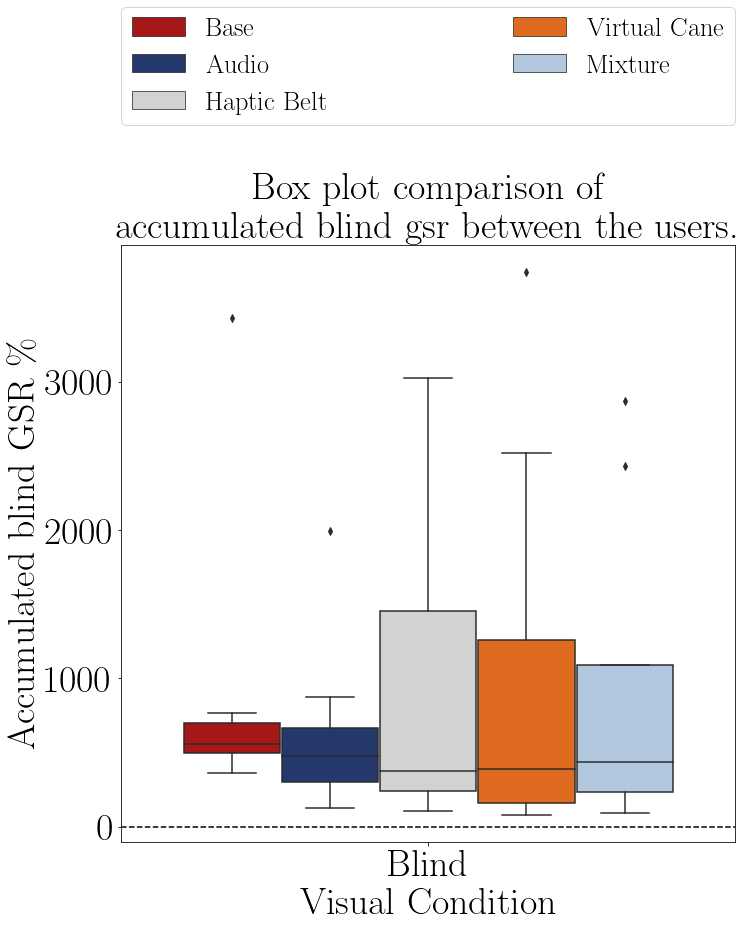
\includegraphics[width = \linewidth]{Resultados/GSR/Figuras/png/boxplot_gsr_sum_blind_scene.png}
        \caption{Boxplot of the average skin conductace of the participants on each method.}
        \label{fig:boxplot_gsr_scene}
    \end{minipage}
    \begin{minipage}{.1\linewidth}
        \hfill
    \end{minipage}
    \begin{minipage}{.45\linewidth}
        \vspace{1.8cm}
        \centering
        %\hspace{-4cm}
        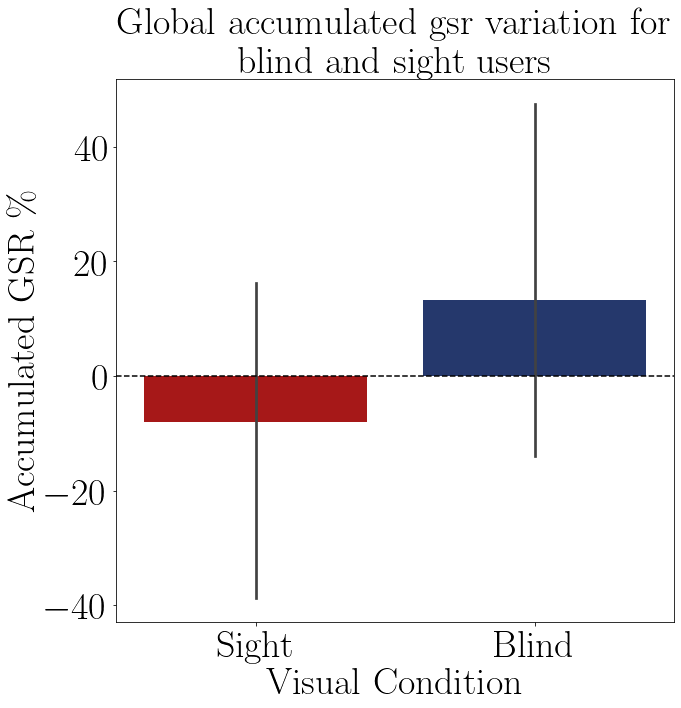
\includegraphics[width = \linewidth]{Resultados/GSR/Figuras/png/barplot_gsr_sum.png}
        \caption{Bar plot of the average GSR of of each group.}
        \label{fig:barplot_gsr_avg}
    \end{minipage}
\end{figure}

\begin{figure}[!htb]
    %\centering
    \begin{minipage}{.45\linewidth}
        \centering
        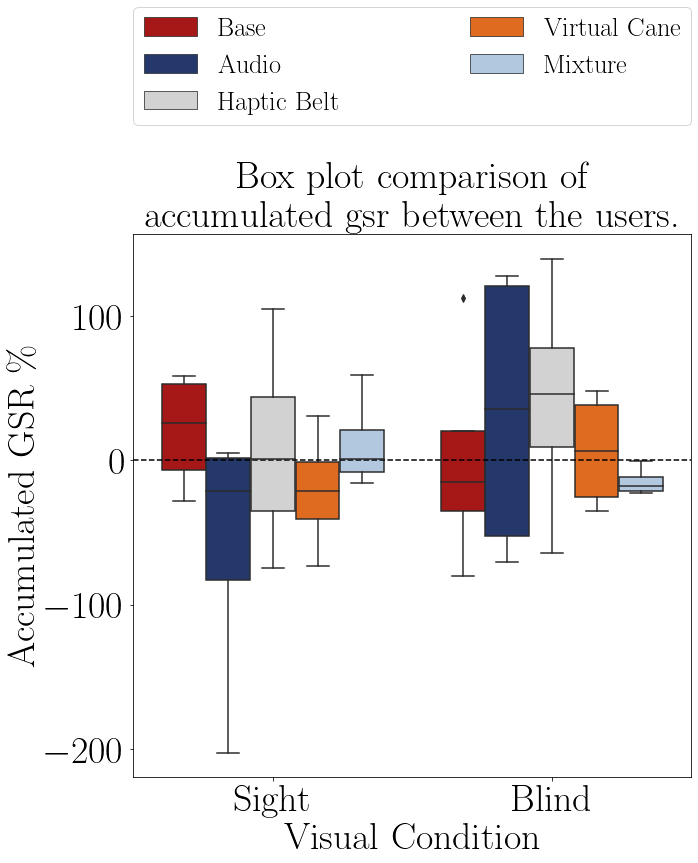
\includegraphics[width = \linewidth]{Resultados/GSR/Figuras/png/boxplot_gsr_sum_scene.png}
        \caption{Boxplot of the average skin conductace of the participants on each method.}
        \label{fig:boxplot_gsr_scene}
    \end{minipage}
    \begin{minipage}{.1\linewidth}
        \hfill
    \end{minipage}
    \begin{minipage}{.45\linewidth}
        \vspace{1.8cm}
        \centering
        %\hspace{-4cm}
        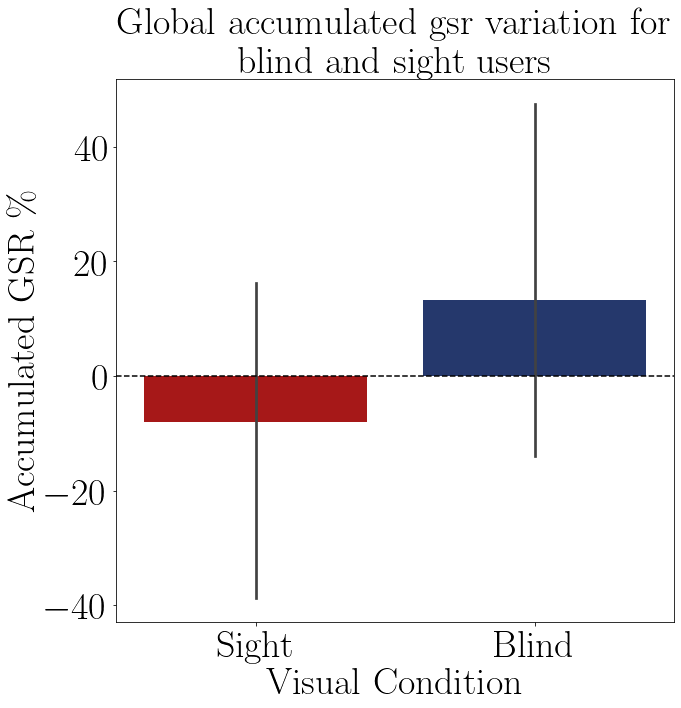
\includegraphics[width = \linewidth]{Resultados/GSR/Figuras/png/barplot_gsr_sum.png}
        \caption{Bar plot of the average GSR of of each group.}
        \label{fig:barplot_gsr_avg}
    \end{minipage}
\end{figure}

%The Table \ref{tab:gsr_avg_table_def2} shows the variation of the heartbeat in each round of each group. It is also possible to notice the same increase noticed before.


\begin{table}[!htb]
\centering
\caption{Accumulated GSR variation in relation to the baseline in each round.}
\label{tab:gsr_sum_table_etp}
\begin{tabular}{lllrrrrrr}
\toprule
    &       &        &      Base &     Audio & \begin{tabular}[c]{@{}l@{}}Haptic\\ Belt\end{tabular} & \begin{tabular}[c]{@{}l@{}}Virtual\\ Cane\end{tabular} &   Mixture \\
Part. & \begin{tabular}[c]{@{}l@{}}Visual\\ Condition\end{tabular} & Round &           &           &                                                       &                                                        &           \\
\midrule
001 & Sight & First &   152.6\% &   121.9\% &                                               174.0\% &                                                261.2\% &    71.9\% \\
    &       & Return &   241.4\% &   128.1\% &                                               135.4\% &                                                182.6\% &   114.5\% \\
001C & Blind & First &   578.3\% &   872.7\% &                                              2261.2\% &                                               2520.5\% &  2866.5\% \\
    &       & Return &   518.2\% &  1990.6\% &                                              3027.1\% &                                               3741.2\% &  2431.1\% \\
002C & Blind & First &  3430.8\% &   423.8\% &                                               105.0\% &                                                 75.7\% &    93.9\% \\
    &       & Return &   674.9\% &   125.9\% &                                               251.8\% &                                                102.5\% &    93.6\% \\
003 & Sight & First &   -49.9\% &    67.4\% &                                               -25.7\% &                                                -41.2\% &   -53.3\% \\
    &       & Return &   -75.6\% &   -69.0\% &                                               -52.8\% &                                                -11.2\% &   -57.7\% \\
003C & Blind & First &   361.4\% &   244.3\% &                                               206.8\% &                                                838.9\% &   646.0\% \\
    &       & Return &   767.4\% &   532.8\% &                                               325.9\% &                                                546.8\% &   514.4\% \\
004 & Sight & First &   886.0\% &   676.1\% &                                               899.3\% &                                                966.4\% &   890.9\% \\
    &       & Return &   894.0\% &   681.9\% &                                               227.2\% &                                                853.4\% &   750.0\% \\
004C & Blind & First &   539.7\% &   593.0\% &                                              1185.5\% &                                                228.6\% &   360.4\% \\
    &       & Return &   432.9\% &   316.4\% &                                               421.8\% &                                                178.2\% &   280.1\% \\
005 & Sight & First &  1198.9\% &  1060.1\% &                                               430.7\% &                                                673.9\% &   233.2\% \\
    &       & Return &   864.7\% &   609.9\% &                                               533.4\% &                                                880.6\% &   220.0\% \\
\bottomrule
\end{tabular}
\end{table}




\begin{table}[!htb]
\centering
\caption{Accumulate GSR variation in relation to the baseline grouped by participant and visual Condition.}
\label{tab:gsr_var_sum_def_blind}
\begin{tabular}{lrrrrr}
\toprule
{} &     Base &    Audio & Haptic Belt & Virtual Cane &  Mixture \\
Visual Condition &          &          &             &              &          \\
\midrule
Blind            &  913.0\% &  637.4\% &     973.1\% &     1029.0\% &  910.8\% \\
\bottomrule
\end{tabular}
\end{table}




\begin{table}[!htb]
\centering
\caption{Accumulate GSR variation in relation to the baseline grouped by participant and visual Condition.}
\label{tab:gsr_var_sum_def}
\begin{tabular}{lrrrrr}
\toprule
{} &    Base &    Audio & Haptic Belt & Virtual Cane &  Mixture \\
Visual Condition &         &          &             &              &          \\
\midrule
Blind            &   0.5\% &   32.3\% &      41.7\% &        6.7\% &  -14.6\% \\
Sight            &  20.7\% &  -59.7\% &       8.0\% &      -21.0\% &   11.5\% \\
\bottomrule
\end{tabular}
\end{table}



%The Shapiro–Wilk normality test on the Table \ref{tab:shapiro_gsr_avg} shows that only the "Audio" method is normally distributed for the "blind" sample while for the "sight" sample only the "Virtual Cane" is not normally distributed

%According to the T-Test presented in the Table \ref{tab:ttest_gsr} there is no difference in the skin conductace  frequency variation between the sample groups.


\begin{table}[!htb]
    \begin{minipage}{.45\linewidth}
        
\centering
\caption{Shapiro test p-value for the gsr accumulated for each method and visual condition}
\label{tab:shapiro_gsr_sum}
\begin{tabular}{lr}
\toprule
                    Method & Shapiro P-Value \\
\midrule
        Base blinded users &         0.000** \\
        Base sighted users &           0.156 \\
       Audio blinded users &         0.015** \\
       Audio sighted users &           0.282 \\
 Haptic Belt blinded users &         0.021** \\
 Haptic Belt sighted users &           0.432 \\
Virtual Cane blinded users &         0.008** \\
Virtual Cane sighted users &           0.158 \\
     Mixture blinded users &         0.006** \\
     Mixture sighted users &           0.060 \\
\bottomrule
\end{tabular}

    \end{minipage}
    \hfill
    \begin{minipage}{.45\linewidth}
        \vspace{-2.75cm}
        
\centering
\caption{T test p-value for the accumulated GSR on each method for blinded users versus sighted users.}
\label{tab:ttest_gsr_sum}
\begin{tabular}{lr}
\toprule
      Method &  T-Test P-Value \\
\midrule
        Base &           0.339 \\
       Audio &           0.383 \\
 Haptic Belt &           0.114 \\
Virtual Cane &           0.286 \\
     Mixture &           0.139 \\
\bottomrule
\end{tabular}

    \end{minipage}
\end{table}

%The Table \ref{tab:repblocanova_gsr} shows the Anova test p-value of the skin conductance frequency of the "blind" sample between the guidance methods presented in the Table \ref{tab:gsr_avg_table}. The p-value indicates that there is at least one method that is statistically equal to one of the other methods.


\begin{table}[!htb]
\centering
\caption{Anova p-value for the accumulated GSR score on each method for blinded users.}
\label{tab:blocanova_gsr_sum}
\begin{tabular}{lrrrrr}
\toprule
            Source &  Squared sum &  DOF & Squared average &     F & \begin{tabular}[c]{@{}l@{}}P-Value \\ $(F_{0} > F)$\end{tabular} \\
\midrule
   Between factors &   727620.618 &    4 &      181905.155 & 0.148 &                                                            0.960 \\
    Between blocks & 18855883.057 &    3 &     6285294.352 & 5.124 &                                                            0.016 \\
Experimental error & 14719563.480 &   12 &     1226630.290 &       &                                                                  \\
    Sampling Error &  6135320.519 &   20 &      306766.026 &       &                                                                  \\
             Total & 40438387.674 &   39 &                 &       &                                                                  \\
\bottomrule
\end{tabular}
\end{table}



%The Table \ref{tab:lsd_gsr} presents the conclusion of a pairwise Fisher LSD test of the blind skin conductance frequency variation between all the guidance methods. The results show that the "Virtual Cane" and the "Mixture" have different variations, but since they are not normally distributed this conclusion can not statistically be made.


\begin{table}[!htb]
\centering
\caption{Cross validation p-value for the accumulated GSR on each method for blinded users.}
\label{tab:lsd_gsr_sum}
\begin{tabular}{rclr}
\toprule
      \multicolumn{3}{c}{Method} &                                       Analysis \\
\midrule
              Base & $X$ & Audio &               $H_0 : \mu_{Base} = \mu_{Audio}$ \\
        Base & $X$ & Haptic Belt &         $H_0 : \mu_{Base} = \mu_{Haptic Belt}$ \\
       Base & $X$ & Virtual Cane &        $H_0 : \mu_{Base} = \mu_{Virtual Cane}$ \\
            Base & $X$ & Mixture &             $H_0 : \mu_{Base} = \mu_{Mixture}$ \\
       Audio & $X$ & Haptic Belt &        $H_0 : \mu_{Audio} = \mu_{Haptic Belt}$ \\
      Audio & $X$ & Virtual Cane &       $H_0 : \mu_{Audio} = \mu_{Virtual Cane}$ \\
           Audio & $X$ & Mixture &            $H_0 : \mu_{Audio} = \mu_{Mixture}$ \\
Haptic Belt & $X$ & Virtual Cane & $H_0 : \mu_{Haptic Belt} = \mu_{Virtual Cane}$ \\
     Haptic Belt & $X$ & Mixture &      $H_0 : \mu_{Haptic Belt} = \mu_{Mixture}$ \\
    Virtual Cane & $X$ & Mixture &     $H_0 : \mu_{Virtual Cane} = \mu_{Mixture}$ \\
\bottomrule
\end{tabular}
\end{table}



%According to the Anova test at Table \ref{tab:repblocanova_gsr} and the LSD test at \ref{tab:lsd_gsr} only the "Virtual Cane" and the "Mixture" method provoked a different reaction than the "Base" method, but since the Shapiro test at the Table \ref{tab:shapiro_gsr_avg} showed that they are not normally distributed, than this conclusion has no foundation.



\FloatBarrier

